        %%******************************************%%
        %%                                          %%
        %%        Modello di tesi di laurea         %%
        %%            di Andrea Giraldin            %%
        %%                                          %%
        %%             2 novembre 2012              %%
        %%                                          %%
        %%******************************************%%


% I seguenti commenti speciali impostano:
% 1. 
% 2. PDFLaTeX come motore di composizione;
% 3. tesi.tex come documento principale;
% 4. il controllo ortografico italiano per l'editor.

% !TEX encoding = UTF-8
% !TEX TS-program = pdflatex
% !TEX root = tesi.tex
% !TEX spellcheck = it-IT

%**************************************************************
% Configurazione per PDF-A
%**************************************************************

\RequirePackage{filecontents}
\begin{filecontents*}{\jobname.xmpdata}
\Title{SMacs SMart city system - Sviluppo di un'app multipiattaforma}
\Author{Tommaso Azzalin}
\Language{it-IT}
\Subject{Il presente documento descrive il lavoro svolto durante il periodo di stage, della durata di circa trecento ore, dal laureando Tommaso Azzalin presso l'azienda TEC Systems Engineering S.r.l.}
\Keywords{stage\sep tesi\sep laurea\sep triennale\sep flutter\sep dart\sep applicazione\sep multipiattaforma}
\end{filecontents*}

%**************************************************************
% Inizio documento
%************************************************************** 

\documentclass[10pt,                    % corpo del font principale
               a4paper,                 % carta A4
               twoside,                 % impagina per fronte-retro
               openright,               % inizio capitoli a destra
               english,                 
               italian,
               rgb,hyperref,rgb,hyperref,dvipsnames % config per usare xcolor e pdfx assieme   
               ]{book}    

%**************************************************************
% Importazione package
%************************************************************** 

%\usepackage{amsmath,amssymb,amsthm}    % matematica

\usepackage{colorprofiles}              % importa i profili colore e altri package già importati qui sotto

\usepackage[a-2b,mathxmp]{pdfx}[2019/03/10] % package per PDF/A e specificata che la versione minima deve essere stata pubblicata dopo la data indicata

\usepackage[T1]{fontenc}                % codifica dei font:
                                        % NOTA BENE! richiede una distribuzione *completa* di LaTeX

\usepackage[utf8]{inputenc}             % codifica di input; anche [latin1] va bene
                                        % NOTA BENE! va accordata con le preferenze dell'editor

\usepackage[english, italian]{babel}    % per scrivere in italiano e in inglese;
                                        % l'ultima lingua (l'italiano) risulta predefinita

\usepackage{bookmark}                   % segnalibri

\usepackage{caption}                    % didascalie

\usepackage{chngpage,calc}              % centra il frontespizio

\usepackage{csquotes}                   % gestisce automaticamente i caratteri (")

\usepackage{emptypage}                  % pagine vuote senza testatina e piede di pagina

\usepackage{epigraph}			% per epigrafi

\usepackage{eurosym}                    % simbolo dell'euro

%\usepackage{indentfirst}               % rientra il primo paragrafo di ogni sezione

\usepackage{graphicx}                   % immagini

% \usepackage{hyperref}                   % collegamenti ipertestuali

\usepackage[binding=5mm]{layaureo}      % margini ottimizzati per l'A4; rilegatura di 5 mm

\usepackage{listings}                   % codici

\usepackage{microtype}                  % microtipografia

\usepackage{mparhack,fixltx2e,relsize}  % finezze tipografiche

\usepackage{nameref}                    % visualizza nome dei riferimenti                                      

\usepackage[font=small]{quoting}        % citazioni

\usepackage{subfig}                     % sottofigure, sottotabelle

\usepackage[italian]{varioref}          % riferimenti completi della pagina

% \usepackage[dvipsnames]{xcolor}         % colori

\usepackage{booktabs}                   % tabelle                                       
\usepackage{tabularx}                   % tabelle di larghezza prefissata                                    
\usepackage{longtable}                  % tabelle su più pagine                                        
\usepackage{ltxtable}                   % tabelle su più pagine e adattabili in larghezza

\usepackage[toc, acronym]{glossaries}   % glossario
                                        % per includerlo nel documento bisogna:
                                        % 1. compilare una prima volta tesi.tex;
                                        % 2. eseguire: makeindex -s tesi.ist -t tesi.glg -o tesi.gls tesi.glo
                                        % 3. eseguire: makeindex -s tesi.ist -t tesi.alg -o tesi.acr tesi.acn
                                        % 4. compilare due volte tesi.tex.

\usepackage[backend=biber,style=verbose-ibid,hyperref,backref]{biblatex}
                                        % eccellente pacchetto per la bibliografia; 
                                        % produce uno stile di citazione autore-anno; 
                                        % lo stile "numeric-comp" produce riferimenti numerici
                                        % per includerlo nel documento bisogna:
                                        % 1. compilare una prima volta tesi.tex;
                                        % 2. eseguire: biber tesi
                                        % 3. compilare ancora tesi.tex.

%**************************************************************
% file contenente le impostazioni della tesi
%**************************************************************

%**************************************************************
% Frontespizio
%**************************************************************

% Autore
\newcommand{\myName}{Tommaso Azzalin}                                    
\newcommand{\myTitle}{SMacs SMart city system - Sviluppo di un'app multipiattaforma}

% Tipo di tesi                   
\newcommand{\myDegree}{Tesi di laurea triennale}

% Università             
\newcommand{\myUni}{Università degli Studi di Padova}

% Facoltà       
\newcommand{\myFaculty}{Corso di Laurea in Informatica}

% Dipartimento
\newcommand{\myDepartment}{Dipartimento di Matematica "Tullio Levi-Civita"}

% Titolo del relatore
\newcommand{\profTitle}{Prof.ssa }

% Relatore
\newcommand{\myProf}{Silvia Crafa}

% Luogo
\newcommand{\myLocation}{Padova}

% Anno accademico
\newcommand{\myAA}{2019-2020}

% Data discussione
\newcommand{\myTime}{24 settembre 2020}

%**************************************************************
% Sommario
%**************************************************************

% Nome azienda
\newcommand{\myCompany}{TEC Systems Engineering S.r.l\@.}

% Nome tutor aziendale
\newcommand{\myTutor}{Andrea Brunello}


%**************************************************************
% Impostazioni di impaginazione
% see: http://wwwcdf.pd.infn.it/AppuntiLinux/a2547.htm
%**************************************************************

\setlength{\parindent}{14pt}   % larghezza rientro della prima riga
\setlength{\parskip}{0pt}   % distanza tra i paragrafi


%**************************************************************
% Impostazioni di biblatex
%**************************************************************
\bibliography{bibliografia} % database di biblatex 

\defbibheading{bibliography} {
    \cleardoublepage
    \phantomsection 
    \addcontentsline{toc}{chapter}{\bibname}
    \chapter*{\bibname\markboth{\bibname}{\bibname}}
}

\setlength\bibitemsep{1.5\itemsep} % spazio tra entry

\DeclareBibliographyCategory{opere}
\DeclareBibliographyCategory{web}

\defbibheading{opere}{\section*{Riferimenti bibliografici}}
\defbibheading{web}{\section*{Siti Web consultati}}


%**************************************************************
% Impostazioni di caption
%**************************************************************
\captionsetup{
    tableposition=top,
    figureposition=bottom,
    font=small,
    format=hang,
    labelfont=bf
}

%**************************************************************
% Impostazioni di glossaries
%**************************************************************

%**************************************************************
% Acronimi
%**************************************************************
\renewcommand{\acronymname}{Acronimi e abbreviazioni}

\newacronym[description={\glslink{apig}{Application Program Interface}}]
    {api}{API}{Application Program Interface}

\newacronym[description={\glslink{umlg}{Unified Modeling Language}}]
    {uml}{UML}{Unified Modeling Language}

\newacronym[description={\glslink{dig}{Dependency Injection}}]
    {di}{DI}{Dependency Injection}

\newacronym[description={\glslink{ideg}{Integrated Development Environment}}]
    {ide}{IDE}{Integrated Development Environment}

\newacronym[description={\glslink{sdkg}{Software Development Kit}}]
    {sdk}{SDK}{Software Development Kit}

\newacronym[description={\glslink{jitg}{Just In Time}}]
    {jit}{JIT}{Just In Time}

\newacronym[description={\glslink{aotg}{Ahead Of Time}}]
    {aot}{AOT}{Ahead Of Time}

\newacronym[description={\glslink{uuidg}{Universally Unique Identifier}}]
    {uuid}{UUID}{Universally Unique Identifier}

\newacronym[description={\glslink{daog}{Data Access Object}}]
    {dao}{DAO}{Data Access Object}

\newacronym[description={\glslink{dtog}{Data Transfer Object}}]
    {dto}{DTO}{Data Transfer Object}

\newacronym[description={\glslink{jsong}{JavaScript Object Notation}}]
    {json}{JSON}{JavaScript Object Notation}

\newacronym[description={\glslink{pojog}{Plain Old Java Object}}]
    {pojo}{POJO}{Plain Old Java Object}

%**************************************************************
% Glossario
%**************************************************************
\renewcommand{\glossaryname}{Glossario}

\newglossaryentry{apig}
{
    name=\glslink{api}{API},
    text=Application Programming Interface,
    sort=api,
    description={In informatica con il termine \emph{Application Programming Interface (API)} (dall'inglese, interfaccia di programmazione di un'applicazione) si indica ogni insieme di procedure disponibili al programmatore, di solito raggruppate a formare un set di strumenti specifici per l'espletamento di un determinato compito all'interno di un certo programma. La finalità è ottenere un'astrazione, di solito tra l'hardware e il programmatore o tra software a basso e quello ad alto livello semplificando così il lavoro di programmazione}
}

\newglossaryentry{umlg}
{
    name=\glslink{uml}{UML},
    text=UML,
    sort=uml,
    description={Nell'ingegneria del software \emph{UML, Unified Modeling Language} (dall'inglese, linguaggio di modellazione unificato) è un linguaggio di modellazione e specifica basato sul paradigma object-oriented. L'\emph{UML} svolge un'importantissima funzione di ``lingua franca'' nella comunità della progettazione e programmazione a oggetti. Gran parte della letteratura di settore usa tale linguaggio per descrivere soluzioni analitiche e progettuali in modo sintetico e comprensibile a un vasto pubblico}
}

\newglossaryentry{dig}
{
    name=\glslink{di}{Dependency Injection},
    text=dependency injection,
    sort=dependencyinjection,
    description={Nell'ingegneria del software per \emph{Dependency Injection} (dall'inglese, iniezione delle dipendenze) è una tecnica che permette a un oggetto di ricevere le proprie dipendenze dall'esterno senza doversene occupare nella sua costruzione. Questo garantisce una migliore separazione dei compiti le classi e una maggiore facilità in fase di test}
}

\newglossaryentry{restg}
{
    name=\glslink{restg}{REST API},
    text=REST API,
    sort=rest,
    description={Le REST API (meglio definite RESTful API) sono API che seguono i principi definiti per l'architettura Representational State Transfer (REST), tipicamente implementate usando HTTP come protocollo di comunicazione}
}

\newglossaryentry{codebaseg}
{
    name=\glslink{codebaseg}{Codebase},
    text=codebase,
    sort=codebase,
    description={Si intende l'intera collezione di codice sorgente necessaria allo sviluppo di un prodotto software}
}

\newglossaryentry{tsg}
{
    name=\glslink{tsg}{TypeScript},
    text=TypeScript,
    sort=typescript,
    description={È un linguaggio di scripting superset di JavaScript che lo sostituisce ma lo integra aggiungendo i tipi statici e permettendo quindi di evitare più errori a runtime grazie alla possibilità di fare una più efficiente analisi statica. Tutto il codice JavaScript è di fatto codice TypeScript valido. Il codice TypeScript può essere a sua volta compilato per produrre del codice JavaScript}
}

\newglossaryentry{ideg}
{
    name=\glslink{ide}{Integrated Development Environment},
    text=IDE,
    sort=ide,
    description={Per \emph{IDE, Integrated Development Environment} (dall'inglese, ambiente di sviluppo integrato) si intende un software utilizzato sia per scrivere il codice sorgente di un prodotto software che per svolgere altre attività che altrimenti richiederebbero l'utilizzo di comandi da terminale, come la compilazione, l'analisi statica, l'esecuzione di test ma anche per svolgere attività come il debugging e il controllo di strumenti correlati come emulatori}
}

\newglossaryentry{frameworkg}
{
    name=\glslink{frameworkg}{Framework},
    text=framework,
    sort=framework,
    description={Un \emph{framework} è un insieme di strumenti software che forniscono allo sviluppatore utilizzatore una maggiore facilità di accesso a certe funzionalità di un linguaggio di programmazione o di un ambiente, come per esempio un sistema operativo}
}

\newglossaryentry{sdkg}
{
    name=\glslink{sdkg}{Software Development Kit},
    text=Software Development Kit,
    sort=sdk,
    description={Per \emph{SDK, Software Development Kit} (dall'inglese, kit per lo sviluppo software) si intende un insieme di strumenti per lo sviluppo e il rilascio di software che lo utilizza. Un SDK contiene ciò che normalmente contiene anche un framework, ma include anche la documentazione e gli strumenti per poter compilare e/o eseguire il codice delle applicazioni che vengono scritte con le librerie presenti nel SDK}
}

\newglossaryentry{assetg}
{
    name=\glslink{assetg}{Asset},
    text=asset,
    sort=asset,
    description={Un \emph{asset} in \emph{Flutter} è un file multimediale, un file di testo oppure un font che viene dichiarato nella configurazione di un progetto e caricato all'avvio dell'applicazione. Gli \emph{asset} sono disponibili in sola lettura}
}

\newglossaryentry{jitg}
{
    name=\glslink{jitg}{Just In Time},
    text=Just In Time,
    sort=jit,
    description={Per \emph{JIT, Just In Time} (dall'inglese, appena in tempo) si intende un tipo di compilatore che compila il codice sorgente a runtime (ovvero lo interpreta)}
}

\newglossaryentry{aotg}
{
    name=\glslink{aotg}{Ahead Of Time},
    text=Ahead Of Time,
    sort=aot,
    description={Per \emph{AOT, Ahead Of Time} (dall'inglese, prima del tempo) si intende un tipo di compilatore che compila il codice sorgente convertendolo in codice macchina in modo che il sistema ospite possa eseguirlo nativamente (ossia senza virtualizzazione)}
}

\newglossaryentry{bestpracticeg}
{
    name=\glslink{bestpracticeg}{Best practice},
    text=best practice,
    sort=bestpractice,
    description={Una \emph{best practice} (dall'inglese, buona pratica) è un modo di agire che ha dimostrato nel tempo di essere il migliore in un certo ambito}
}

\newglossaryentry{uuidg}
{
    name=\glslink{uuidg}{Universally Unique Identifier},
    text=UUID,
    sort=uuid,
    description={Un \emph{UUID, Universally Unique Identifier} (dall'inglese, identificativo univoco universale) rappresenta un tipo di identificativo per identificare univocamente un'informazione in assenza di un sistema di coordinamento. Ciò significa che entità completamente distinte e di sistemi diversi sono comunque identificabili se hanno un UUID, in quanto - in pratica - univoco}
}

\newglossaryentry{dtog}
{
    name=\glslink{dtog}{Data Transfer Object},
    text=DTO,
    sort=datatransferobject,
    description={Un \emph{DTO, Data Transfer Object} (dall'inglese, oggetto per il trasferimento dati) rappresenta un tipo di classe molto semplice contenente dati ottenuti da remoto o da altre API strutturati per un loro agevole passaggio fra varie entità all'interno dell'architettura software}
}

\newglossaryentry{daog}
{
    name=\glslink{daog}{Data Access Object},
    text=DAO,
    sort=dataaccessobject,
    description={Un \emph{DAO, Data Access Object} (dall'inglese, oggetto per l'accesso ai dati) rappresenta un tipo di classe in cui vengono elaborati dati ottenuti da remoto, da altre API, ricevuti come argomento sotto forma di DTO e ritorna altri dati, spesso sotto forma di DTO}
}

\newglossaryentry{jsong}
{
    name=\glslink{jsong}{JavaScript Object Notation},
    text=JSON,
    sort=javascriptobjectnotation,
    description={Per \emph{JSON} si intende un tipo di notazione tipicamente usata per rappresentare in JavaScript gli oggetti, usata comunemente dalle API di tipo RESTful come formato di interscambio dati, al pari di altri come ad esempio XML}
}

\newglossaryentry{designpatterng}
{
    name=\glslink{designpatterng}{Design pattern},
    text=design pattern,
    sort=designpattern,
    description={Un \emph{design pattern} è una soluzione software generica e quindi riutilizzabile che risolve in un modo efficiente ed efficace un problema che si presenta spesso durante la progettazione di un sistema software. I design pattern principali sono quelli creazionali (che risolvono problemi comuni nella creazione di oggetti), strutturali (che implementano soluzioni a problemi nella gestione di oggetti), comportamentali (che offrono soluzioni all'utilizzo di oggetti)}
}

\newglossaryentry{pojog}
{
    name=\glslink{pojog}{POJO},
    text=POJO,
    sort=pojo,
    description={Un \emph{Plain Old Java Object, POJO} è un tipo di classe che viene definita in Java in cui non ci sono dipendenze in ingresso da altre librerie, possibilmente non hanno annotazioni e sono serializzabili, e le proprietà sono accessibili attraverso \emph{getter} e \emph{setter}}
}


% acronimo più glossario
\newacronym[description={\glslink{testoConG}{TestoXEsteso}}]
    {TESTO_DA_CATTURARE}{ACRONIMO}{TestoXEsteso}

\newglossaryentry{testoConG}
{
    name=\glslink{TESTO_DA_CATTURARE}{ACRONIMO},
    text=TestoXEsteso,
    sort=TESTO_DA_ORDINARE,
    description={Descrizione}
}

% solo glossario
\newglossaryentry{testoConGg}
{
    name=\glslink{testoConG}{TestoXEsteso},
    text= TestoXEsteso,
    sort=TESTO_DA_ORDINARE,
    description={Descrizione}
} % database di termini
\makeglossaries


%**************************************************************
% Impostazioni di graphicx
%**************************************************************
\graphicspath{{immagini/}} % cartella dove sono riposte le immagini

%**************************************************************
% Impostazioni di longtable
%**************************************************************

\usepackage{array} % colonne custom per tabelle

\newcolumntype{L}[1]{>{\raggedright\let\newline\\\arraybackslash\hspace{0pt}}m{#1}}
\newcolumntype{C}[1]{>{\centering\let\newline\\\arraybackslash\hspace{0pt}}m{#1}}
\newcolumntype{R}[1]{>{\raggedleft\let\newline\\\arraybackslash\hspace{0pt}}m{#1}}

%**************************************************************
% Impostazioni di hyperref
%**************************************************************
\hypersetup{
    %hyperfootnotes=false,
    %pdfpagelabels,
    %draft,	% = elimina tutti i link (utile per stampe in bianco e nero)
    colorlinks=true,
    linktocpage=true,
    pdfstartpage=1,
    % pdfstartview=FitV,
    pdfstartview=,
    % decommenta la riga seguente per avere link in nero (per esempio per la stampa in bianco e nero)
    %colorlinks=false, linktocpage=false, pdfborder={0 0 0}, pdfstartpage=1, pdfstartview=FitV,
    breaklinks=true,
    pdfpagemode=UseNone,
    pageanchor=true,
    pdfpagemode=UseOutlines,
    plainpages=false,
    bookmarksnumbered,
    bookmarksopen=true,
    bookmarksopenlevel=1,
    hypertexnames=true,
    pdfhighlight=/O,
    %nesting=true,
    %frenchlinks,
    urlcolor=webbrown,
    linkcolor=RoyalBlue,
    citecolor=webgreen,
    %pagecolor=RoyalBlue,
    %urlcolor=Black, linkcolor=Black, citecolor=Black, %pagecolor=Black,
    pdftitle={\myTitle},
    pdfauthor={\textcopyright\ \myName, \myUni, \myFaculty},
    pdfsubject={},
    pdfkeywords={},
    pdfcreator={pdfLaTeX},
    pdfproducer={LaTeX}
}

%**************************************************************
% Impostazioni di itemize
%**************************************************************
\renewcommand{\labelitemi}{$\bullet$}

%\renewcommand{\labelitemi}{$\bullet$}
% \renewcommand{\labelitemii}{$\cdot$}
%\renewcommand{\labelitemiii}{$\diamond$}
%\renewcommand{\labelitemiv}{$\ast$}


%**************************************************************
% Impostazioni di xcolor
%**************************************************************
\definecolor{webgreen}{rgb}{0,.5,0}
\definecolor{webbrown}{rgb}{.6,0,0}



%**************************************************************
% Impostazioni di listings
%**************************************************************
\lstset{
    language=C++,
    keywordstyle=\color{RoyalBlue}, %\bfseries,
    basicstyle=\small\ttfamily,
    emph={
        % C++
        int,char,double,float,unsigned,string,cstdlib,
        % Qt
        QString,QWidget,QPushButton,QApplication,ExampleApp,
        % Dart
        var,final,mixin,with,extends,implements
        % Flutter
    },
    emphstyle=\color{RoyalBlue},
    directivestyle=\color{black},
    commentstyle=\color{webgreen}\ttfamily,
    stringstyle=\ttfamily,
    numbers=left,
    numberstyle=\scriptsize, %\tiny
    stepnumber=1,
    numbersep=8pt,
    showstringspaces=false,
    breaklines=true,
    frameround=ffff,
    frame=single
} 


%**************************************************************
% Altro
%**************************************************************

\newcommand{\omissis}{[\dots\negthinspace]} % produce [...]

% eccezioni all'algoritmo di sillabazione
\hyphenation
{
    az-za-lin
    en-gi-neer-ing
    ob-serv-er
}

\newcommand{\sectionname}{sezione}
\addto\captionsitalian{\renewcommand{\figurename}{Figura}
                       \renewcommand{\tablename}{Tabella}}

\newcommand{\glsfirstoccur}{\ap{{[g]}}}

\newcommand{\intro}[1]{\emph{\textsf{#1}}}

%**************************************************************
% Environment per ``rischi''
%**************************************************************
\newcounter{riskcounter}                % define a counter
\setcounter{riskcounter}{0}             % set the counter to some initial value

%%%% Parameters
% #1: Title
\newenvironment{risk}[1]{
    \refstepcounter{riskcounter}        % increment counter
    \par \noindent                      % start new paragraph
    \textbf{\arabic{riskcounter}. #1}   % display the title before the 
                                        % content of the environment is displayed 
}{
    \par\medskip
}

\newcommand{\riskname}{Rischio}

\newcommand{\riskdescription}[1]{\textbf{\\Descrizione:} #1.}

\newcommand{\risksolution}[1]{\textbf{\\Soluzione:} #1.}

%**************************************************************
% Environment per ``use case''
%**************************************************************
\newcounter{usecasecounter}             % define a counter
\setcounter{usecasecounter}{0}          % set the counter to some initial value

%%%% Parameters
% #1: ID
% #2: Nome
\newenvironment{usecase}[2]{
    \renewcommand{\theusecasecounter}{\usecasename #1}  % this is where the display of 
                                                        % the counter is overwritten/modified
    \refstepcounter{usecasecounter}             % increment counter
    \vspace{10pt}
    \par \noindent                              % start new paragraph
    {\large \textbf{\usecasename #1 - #2}}       % display the title before the 
                                                % content of the environment is displayed 
    \medskip
}{
    \medskip
}

\newcommand{\usecasename}{UC}

\newcommand{\usecaseprimaryactors}[1]{\textbf{\\Attori principali:} #1. \vspace{4pt}}
\newcommand{\usecasesecondaryactors}[1]{\textbf{\\Attori secondari:} #1. \vspace{4pt}}
\newcommand{\usecasepre}[1]{\textbf{\\Precondizioni:} #1 \vspace{4pt}}
\newcommand{\usecasedesc}[1]{\textbf{\\Scenario principale:} #1 \vspace{4pt}}
\newcommand{\usecasepost}[1]{\textbf{\\Postcondizioni:} #1 \vspace{4pt}}
\newcommand{\usecasegen}[1]{\textbf{\\Generalizzazioni:} #1 \vspace{4pt}}
\newcommand{\usecaseext}[1]{\textbf{\\Estensioni:} #1 \vspace{4pt}}

%**************************************************************
% Environment per ``namespace description''
%**************************************************************

\newenvironment{namespacedesc}{
    \vspace{10pt}
    \par \noindent                              % start new paragraph
    \begin{description} 
}{
    \end{description}
    \medskip
}

\newcommand{\classdesc}[2]{\item[\textbf{#1:}] #2}

                     % file con le impostazioni personali

\begin{document}
%**************************************************************
% Materiale iniziale
%**************************************************************
\frontmatter
% !TEX encoding = UTF-8
% !TEX TS-program = pdflatex
% !TEX root = ../tesi.tex

%**************************************************************
% Frontespizio 
%**************************************************************
\begin{titlepage}

\begin{center}

\begin{LARGE}
\textbf{\myUni}\\
\end{LARGE}

\vspace{10pt}

\begin{Large}
\textsc{\myDepartment}\\
\end{Large}

\vspace{10pt}

\begin{large}
\textsc{\myFaculty}\\
\end{large}

\vspace{30pt}
\begin{figure}[htbp]
\begin{center}

\includegraphics[height=6cm]{logo-unipd}
\end{center}
\end{figure}
\vspace{30pt} 

\begin{LARGE}
\begin{center}
\textbf{\myTitle}\\
\end{center}
\end{LARGE}

\vspace{10pt} 

\begin{large}
\textsl{\myDegree}\\
\end{large}

\vspace{40pt} 

\begin{large}
\begin{flushleft}
\textit{Relatrice}\\ 
\vspace{5pt} 
\profTitle \myProf
\end{flushleft}

\vspace{0pt} 

\begin{flushright}
\textit{Laureando}\\ 
\vspace{5pt} 
\myName
\end{flushright}
\end{large}

\vspace{40pt}

\line(1, 0){338} \\
\begin{normalsize}
\textsc{Anno Accademico \myAA}
\end{normalsize}

\end{center}
\end{titlepage} 
% !TEX encoding = UTF-8
% !TEX TS-program = pdflatex
% !TEX root = ../tesi.tex

%**************************************************************
% Colophon
%**************************************************************
\clearpage
\phantomsection
\thispagestyle{empty}

\hfill

\vfill

\noindent\myName: \textit{\myTitle,}
\myDegree,
\textcopyright\ \myTime.
% !TEX encoding = UTF-8
% !TEX TS-program = pdflatex
% !TEX root = ../tesi.tex

%**************************************************************
% Dedica
%**************************************************************
\cleardoublepage
\phantomsection
\thispagestyle{empty}
\pdfbookmark{Dedica}{Dedica}

\vspace*{3cm}

\begin{center}
"La soluzione brillante di un falso problema può essere peggiore che nessuna soluzione. Tutto sta nel risolvere il problema giusto." \\ \medskip
--- Donald Norman
\end{center}

\medskip

\begin{center}
Dedicato a tutti gli insegnanti che hanno contribuito a formare la persona che sono oggi.
\end{center}

% !TEX encoding = UTF-8
% !TEX TS-program = pdflatex
% !TEX root = ../tesi.tex

%**************************************************************
% Sommario
%**************************************************************
\cleardoublepage
\phantomsection
\pdfbookmark{Sommario}{Sommario}
\begingroup
\let\clearpage\relax
\let\cleardoublepage\relax
\let\cleardoublepage\relax

\chapter*{Sommario}

Il presente documento descrive il lavoro svolto durante il periodo di stage, della durata di circa trecento ore, dal laureando \myName{} presso l'azienda \myCompany{}\\
L'obiettivo dello stage è stato realizzare un’applicazione mobile multipiattaforma (per sistemi operativi Android e iOS) per la gestione di impianti semaforici (e altre componenti per la regolazione del traffico) che:
\begin{itemize}
    \item[-] si basasse sull'applicazione già in uso presso l'azienda, implementata per solo sistema operativo Android;
    \item[-] si interfacciasse con un web server tramite API REST permettendo il reperimento dei dati da visualizzare all’utente e la loro modifica;
    \item[-] si attivasse autonomamente in background con intervalli di tempi predefiniti per verificare la presenza di nuovi dati per l’utente.
\end{itemize}

%\vfill
%
%\selectlanguage{english}
%\pdfbookmark{Abstract}{Abstract}
%\chapter*{Abstract}
%
%\selectlanguage{italian}

\endgroup			

\vfill


% !TEX encoding = UTF-8
% !TEX TS-program = pdflatex
% !TEX root = ../tesi.tex

%**************************************************************
% Ringraziamenti
%**************************************************************
\cleardoublepage
\phantomsection
\pdfbookmark{Ringraziamenti}{ringraziamenti}

% \begin{flushright}{
% 	\slshape    
% 	``Altra citazione da mettere''} \\ 
% 	\medskip
%     --- altro autore da mettere
% \end{flushright}


\bigskip

\begingroup
\let\clearpage\relax
\let\cleardoublepage\relax
\let\cleardoublepage\relax

\chapter*{Ringraziamenti}

\noindent \textit{Innanzitutto, vorrei esprimere la mia gratitudine alla Prof.ssa \myProf{}, relatrice della mia tesi, e ad \myTutor{}, il mio tutor aziendale, per l'aiuto e il sostegno fornitomi durante lo svolgimento dello stage e della stesura di questa relazione.}\\

\noindent \textit{Desidero ringraziare i miei genitori per il loro sostegno e aiuto, standomi vicini in ogni momento durante gli anni di studio.}\\

\noindent \textit{Ho desiderio di ringraziare poi i miei compagni e amici, conosciuti in questi anni all'Università, per l'aiuto e il sostegno ricevuto.}\\

\noindent \textit{Infine, ringrazio Bianca, per avermi quotidianamente ascoltato e aiutato, soprattutto nei momenti più impegnativi.}\\
\bigskip

\noindent\textit{\myLocation, \myTime}
\hfill \myName

\endgroup


% !TEX encoding = UTF-8
% !TEX TS-program = pdflatex
% !TEX root = ../tesi.tex

%**************************************************************
% Indici
%**************************************************************
\cleardoublepage
\pdfbookmark{\contentsname}{tableofcontents}
\setcounter{tocdepth}{2}
\tableofcontents
%\markboth{\contentsname}{\contentsname} 
\clearpage

\begingroup 
    \let\clearpage\relax
    \let\cleardoublepage\relax
    \let\cleardoublepage\relax
    %*******************************************************
    % Elenco delle figure
    %*******************************************************    
    \phantomsection
    \pdfbookmark{\listfigurename}{lof}
    \listoffigures

    \vspace*{8ex}

    %*******************************************************
    % Elenco delle tabelle
    %*******************************************************
    \phantomsection
    \pdfbookmark{\listtablename}{lot}
    \listoftables
        
    \vspace*{8ex}
\endgroup

\cleardoublepage

\cleardoublepage

%**************************************************************
% Materiale principale
%**************************************************************
\mainmatter
% !TEX encoding = UTF-8
% !TEX TS-program = pdflatex
% !TEX root = ../tesi.tex

%**************************************************************
\chapter{Introduzione}
\label{cap:introduzione}
%**************************************************************

\intro{
    In questo capitolo introduttivo viene illustrata l'idea che ha portato alla scelta del progetto di stage presso \myCompany{}, introdotto brevemente il prodotto realizzato e analizzati gli obiettivi raggiunti.
    Infine, viene illustrato come i contenuti nel presente documento sono stati organizzati.
}\\

%**************************************************************
\section{L'idea}
\label{sec:idea}
In un mondo in cui l'informatica e le telecomunicazioni (in inglese, \emph{Information and Communication Technologies - ICT}) pervadono sempre più ogni ambito, automatizzando e migliorando, in efficienza ed efficacia, i sistemi in cui vengono applicate, i sistemi di trasporto non potevano non essere parte di questo cambiamento.\\
L'ingegneria dei trasporti è quella parte dell'ingegneria che si occupa di creare soluzioni per il trasporto delle merci, delle persone, tra cui la realizzazione di infrastrutture e veicoli.\\
L'innovazione tecnologica ha fatto sì che i sistemi di trasporto (in inglese, \emph{Transportation Systems}) venissero integrati con la telematica, creando dei "sistemi di trasporto intelligenti" (in inglese, \emph{Intelligent Transportation Systems}).\\
Un \emph{Intelligent Transportation System (ITS)} è quindi il risultato dell'applicazione dell'ICT alle infrastrutture per i trasporti ed ai veicoli, al fine di rendere più efficiente i sistemi di trasporto.\\
Più in dettaglio, possiamo scomporre il termine \emph{ITS} e analizzarlo parola per parola:
\begin{itemize}
    \item \emph{Intelligent}, si riferisce ad entità che hanno l'abilità di apprendere, adattarsi a nuove situazioni e usare le informazioni che raccolgono per migliorare la loro efficienza operativa;
    \item \emph{Transportation}, entità che collaborano per il movimento di merci e persone;
    \item \emph{System}, entità che svolgono attività in base a regolamenti interni e con un fine comune.
\end{itemize}
Un \emph{ITS} è importante per molteplici ragioni:
\begin{itemize}
    \item per ridurre le congestioni del traffico;
    \item per permettere di risparmiare tempo e consumare meno carburante;
    \item per ridurre le emissioni inquinanti;
    \item per permettere un abbassamento del numero di incidenti;
    \item per favorire una rete di trasporti in generale più sicura e che garantisca meno stress.
\end{itemize}
Con un \emph{ITS} è possibile:
\begin{itemize}
    \item gestire le Zone a Traffico Limitato (ZTL);
    \item gestire il traffico e il transito dei veicoli;
    \item dare priorità al transito dei mezzi pubblici;
    \item raccogliere dati sul traffico;
    \item dare informazioni in tempo reale tramite segnalatori acustici e visivi;
    \item gestire i parcheggi e la loro capienza;
    \item gestire le stazioni meteorologiche;
    \item controllare la qualità dell'aria;
    \item collezionare dati per inviarli a dei server per poterli analizzare e monitorare mediante sale di controllo.
\end{itemize}

%**************************************************************
\section{L'azienda}
\label{sec:azienda}

\myCompany{} è un'azienda con sede a Padova, nata nel 2007 dall'idea dei suoi soci fondatori, ingegneri impiegati nel campo dell'ICT e della progettazione di sistemi per il controllo e gestione del traffico.
È partner esclusivo del Gruppo La Semaforica, per cui produce Intelligent Transportation System (ITS).\\
Si propone per la fornitura di strumenti potenti e flessibili a Pubbliche Amministrazioni, integratori di sistemi, aziende private e professionisti che vogliono mettere in atto sistemi efficienti senza considerare dettagli implementativi.
Oltre a questo, intende offrire prodotti di alta qualità e assistenza tecnica di alto livello.\\
Tutto questo per affrontare in modo innovativo i problemi della mobilità pubblica e privata, da un punto di vista della sicurezza, dell'efficienza, dell'efficacia e nel rispetto dell'ambiente.

%**************************************************************
\section{Il progetto di stage}
\label{sec:progetto-stage}

Il progetto pensato per lo stage è stato la realizzazione di un'applicazione multipiattaforma (per dispositivi con sistema operativo Android o iOS), per la gestione di impianti semaforici (e altre componenti per la regolazione del traffico), che:
\begin{itemize}
    \item si basi sull'applicazione già in uso presso l'azienda, implementata per solo sistema operativo Android;
    \item si interfacci con i web server aziendali tramite \gls{restg}, permettendo il reperimento dei dati da visualizzare all'utente e la loro modifica;
    \item si attivi autonomamente in background con intervalli di tempi predefiniti per verificare la presenza di nuovi dati per l'utente.
\end{itemize}

%**************************************************************
\section{Raggiungimento degli obiettivi}
\label{sec:raggiungimento-obiettivi}

Lo stage è stato svolto dal 23 giugno al 31 agosto 2020, per un totale di 320 ore di lavoro effettive (40 ore settimanali per 8 settimane).\\
Gli obiettivi pianificati per il progetto di stage, indicati nella precedente sezione "\hyperref[sec:progetto-stage]{Il progetto di stage}" e i casi d'uso analizzati nella prima settimana di stage raccolti in "\hyperref[cap:analisi-dei-requisiti]{Analisi dei requisiti}", sono stati tutti raggiunti.
Il tutor aziendale \myTutor{} ha inoltre espresso la sua soddisfazione per il prodotto realizzato, convinto che possa essere inizialmente messo in prova su una piccola parte dei loro clienti, per poi espanderla mano a mano che le funzionalità vengono integrate e potendo quindi sostituire l'applicazione attualmente in uso.\\

%**************************************************************
\section{Organizzazione del testo}
\label{sec:organizzazione-testo}

\begin{description}
    \item[{\hyperref[cap:introduzione]{Il primo capitolo}}] offre una panoramica sul contesto applicativo in cui si pone il progetto realizzato proposto dall'azienda ospitante.

    \item[{\hyperref[cap:descrizione-stage]{Il secondo capitolo}}] descrive come è stato organizzato lo stage, la pianificazione del lavoro e gli obiettivi da raggiungere.
    
    \item[{\hyperref[cap:scelta-tecnologie]{Il terzo capitolo}}] spiega come è stata fatta la scelta delle tecnologie usate per realizzare il prodotto di stage.
    
    \item[{\hyperref[cap:confronto-paradigmi]{Il quarto capitolo}}] tratta della differenza fra il paradigma di programmazione impiegato dalle tecnologie scelte e quello usato in altre tecnologie apprese nel corso degli studi;
    
    \item[{\hyperref[cap:dependency-injection]{Il quinto capitolo}}] illustra della differenza fra come la \gls{di} viene implementata nelle tecnologie scelte e in quelle di altre tecnologie apprese nel corso degli studi.
    
    \item[{\hyperref[cap:prodotto-stage]{Il sesto capitolo}}] dimostra come è stata scelta l'architettura impiegata per realizzare il prodotto finale e come è stato implementato.

    \item[{\hyperref[cap:conclusioni]{Il settimo e ultimo capitolo}}] propone infine alcune conclusioni sull'esperienza svolta, tra cui delle valutazioni sullo stage e sul prodotto realizzato.
\end{description}
Gli acronimi, le abbreviazioni e i termini ambigui o di uso non comune menzionati vengono definiti nel glossario, situato alla fine del presente documento.             % Introduzione
% !TEX encoding = UTF-8
% !TEX TS-program = pdflatex
% !TEX root = ../tesi.tex

%**************************************************************
\chapter{Descrizione dello stage}
\label{cap:descrizione-stage}
%**************************************************************

\intro{
    In questa sezione viene trattato come è stato svolto lo stage presso \myCompany{}, toccando aspetti legati alla comunicazione e agli obiettivi dello stage pianicati, discutendo anche dei possibili rischi che si sarebbero potuti riscontrare.
}\\

%**************************************************************
\section{Svolgimento}
\label{sec:svolgimento}

Lo stage è stato svolto, su accordo, completamente da remoto per evitare spiacevoli situazioni di contagio dovute all'emergenza sanitaria in corso.\\
Nonostante questo, i contatti con il tutor aziendale sono stati quotidiani.\\
Le comunicazioni sono avvenute principalmente attraverso un gruppo su WhatsApp, sia per aggiornamenti sullo stato dei lavori, che per richieste di chiarimenti e aiuto.\\
Per le video-chiamate è stato invece usato il software Zoom, utile principalmente in situazioni di richiesta di aiuto più importanti, dove il semplice scambio di messaggi non avrebbe portato a risultati soddisfacenti.

%**************************************************************
\section{Requisiti e obiettivi finali}
\label{sec:requisiti-obiettivi-finali}

Gli obiettivi definiti per lo stage erano i seguenti:
\begin{itemize}
    \item sviluppare un'applicazione multipiattaforma sulla base dell'applicazione già in uso presso l'azienda, disponibile per solo sistema operativo Android;
    \item l'applicazione doveva reperire i dati dai server aziendali attraverso \gls{restg};
    \item l'applicazione doveva inoltre attivarsi in background, su richiesta dell'utente, ad intervalli di tempo predefiniti per verificare la presenza di nuove informazioni da comunicare.
\end{itemize}
Oltre a questi obiettivi elencati, obbligatori, ce n'erano due ulteriori, ma secondari:
\begin{itemize}
    \item internazionalizzare l'applicazione (in italiano e in inglese, ma facendo in modo che altre lingue possano essere aggiunte);
    \item comprendere come generare i pacchetti da distribuire ai clienti dell'azienda per l'installazione dell'applicazione.
\end{itemize}
Un obiettivo che si è ritenuto necessario introdurre durante lo stage, senza però formalizzarlo, è stato quello di effettuare un restyling grafico dell'interfaccia utente dell'applicazione, con un occhio sia all'esperienza utente che all'accessibilità. Alcune considerazioni su questo punto vengono proposte in \hyperref[sec:confronto-precedente-app-nuova]{Confronto fra la precedente app e quella nuova}.\\
Per i requisiti basati sui casi d'uso elaborati durante lo stage, consultare l'"\hyperref[cap:analisi-dei-requisiti]{Analisi dei requisiti}" in appendice.

%**************************************************************
\section{Rischi riscontrabili}
\label{sec:rischi}

Durante la prima settimana di stage si è fatta una riflessione su quali fossero i possibili rischi riscontrabili nello sviluppo del progetto proposto dall'azienda.
Si è quindi proceduto a elaborare delle possibili soluzioni per far fronte a tali rischi.\\

\begin{risk}{Ritardo nella pianificazione dovuto a una sezione dell'applicazione}
    \riskdescription{alcune sezioni dell'applicazione potrebbero richiedere, per loro natura, un maggior dispendio di tempo sia nella loro progettazione che nel loro sviluppo}
    \risksolution{fissare una scadenza a brevissimo termine entro cui provare a risolvere il problema che sta bloccando il proseguimento dei lavori. Se entro quella scadenza non si è risolto, procedere con altre sezioni meno impegnative per guadagnare il tempo speso}
    \label{risk:ritardo-pianificazione} 
\end{risk}

\begin{risk}{Difficoltà di comprensione delle REST API aziendali}
    \riskdescription{le \gls{restg} aziendali, essendo strettamente collegate ad alcuni aspetti dell'hardware gestito dall'azienda e ricche di glossario specifico nella documentazione, potrebbero essere difficilmente comprensibili}
    \risksolution{avvisare subito il tutor aziendale per chiedere spiegazioni ed esempi, qualora necessario}
    \label{risk:difficolta-comprensione} 
\end{risk}

\begin{risk}{Difficoltà nell'utilizzo delle tecnologie}
    \riskdescription{non avendo molta esperienza con le tecnologie in uso per lo sviluppo dell'applicazione è possibile che alcune parti siano di difficile realizzazione, dovuto anche a una cattiva interpretazione della documentazione}
    \risksolution{avvisare subito il tutor aziendale per chiedere aiuto e cercare di comprendere assieme la documentazione ed arrivare ad una soluzione}
    \label{risk:difficolta-utilizzo-tecnologie} 
\end{risk}

%**************************************************************
\section{Pianificazione}
\label{sec:pianificazione}

Il lavoro è stato suddiviso secondo questa pianificazione:
\begin{itemize}
    \item la prima settimana si sono svolte attività introduttive tra cui un orientamento sul lavoro svolto dall'azienda, l'acquisizione di glossario specifico e l'analisi dell'applicazione attualmente in uso dall'azienda per comprenderne i casi d'uso;
    \item la seconda settimana si è svolta la progettazione dell'interfaccia utente dell'applicazione, prendendo spunto dall'attuale app e cercando, assieme al tutor, di trovare modi per rinnovarla e migliorarla dove possibile; inoltre, si è cercata la miglior architettura per la progettazione dell'app, sia per i tempi a disposizione, che per le necessità;
    \item le altre settimane si è progettata nel dettaglio l'applicazione, basandosi sull'architettura selezionata, cercando di renderla quanto più possibile estendibile per possibili sviluppi futuri; durante le settimane si è provveduto anche a testare man mano le componenti sviluppate per assicurarsi del loro funzionamento;
    \item l'ottava e ultima settimana, oltre a terminare alcune parti mancanti dell'applicazione, si è provveduto alla internazionalizzazione dell'applicazione.
\end{itemize}             % Descrizione dello stage
% !TEX encoding = UTF-8
% !TEX TS-program = pdflatex
% !TEX root = ../tesi.tex

%**************************************************************
\chapter{Scelta delle tecnologie}
\label{cap:scelta-tecnologie}
%**************************************************************

\intro{
    Per la realizzazione del prodotto proposto dall'azienda non è stato richiesta nessuna tecnologia in particolare, per cui in questa sezione viene riproposto il processo decisionale che ha portato alla scelta e al successivo utilizzo di quanto usato durante lo stage.
}\\

%**************************************************************
\section{Applicazione nativa o multipiattaforma?}
\label{sec:nativa-multipiattaforma}

Nonostante il titolo di questa relazione citi \emph{Sviluppo di un'app multipiattaforma}, la scelta di realizzare un'app multipiattaforma è stata presa dopo aver valutato tutti i vantaggi che questa scelta avrebbe potuto portare.
Come è dichiarato nella sezione "\hyperref[sec:requisiti-obiettivi-finali]{Requisiti e obiettivi finali}", l'azienda dispone già di un'applicazione Android e quindi, quando si è discusso del progetto da realizzare per lo stage, è stato proposto di realizzare la sua controparte per iOS.\\
Sviluppare per iOS, ovvero realizzare un'app nativa, ha chiaramente i vantaggi derivati dallo sviluppo proprio per la piattaforma di destinazione, che per lo sviluppatore corrispondono all'accesso diretto a funzionalità del sistema operativo e a una vasta disponibilità di librerie di terze parti, permettendo la creazione di app fluide che possono usare tutte le componenti native offerte direttamente dal sistema operativo.\\
D'altra parte, però, significa apprendere una tecnologia nuova, che è sempre un vantaggio, ma limitata a quel solo scopo.\\
Un altro svantaggio non banale nell'avere un'applicazione sviluppata separatamente per due sistemi diversi è la necessità di avere due \gls{codebaseg} distinti, da mantenere separatamente.
Un ulteriore svantaggio legato intrinsecamente ad iOS è il dover sviluppare, eseguire test, fare debugging e compilazione su un computer con sistema operativo MacOS (che richiede un Mac) e l'\gls{ide} XCode di Apple.\\
Per questi motivi si è optato per realizzare un'app multipiattaforma che permette, oltre a raggiungere l'utenza finora non raggiunta, di andare gradualmente a sostituire la precedente applicazione.
Un punto fondamentale dello sviluppo di applicazioni multipiattaforma è la scelta della tecnologia, in quanto a disposizione per lo sviluppatore ce ne sono molteplici e con diverse caratteristiche.
Tutte queste hanno in comune la possibilità di avere un solo \gls{codebaseg} per entrambe le versione dell'app (per Android e per iOS) e un'interfaccia uniforme fra i vari dispositivi.
Inoltre, non essendo un'applicazione nativa, usa un linguaggio di programmazione non compatibile con i \gls{sdk} messi a disposizione da Google e Apple per lo sviluppo di applicazioni per i loro sistemi operativi. Tipicamente questo linguaggio è JavaScript o il suo superset \gls{tsg}.
Un'importante differenza, o svantaggio, è che utilizzando un \gls{frameworkg} o un linguaggio che non ha accesso nativamente alle funzionalità e alle librerie del sistema operativo deve avere dei modi per astrarle, tramite integrazioni nel \gls{frameworkg} o tramite librerie esterne, spesso non sviluppate dallo stesso team che sviluppa la tecnologia multipiattaforma, richiedendo più attenzione da parte dello sviluppatore.\\
Come è stato detto in precedenza, per questo progetto è stata scelta una tecnologia multipiattaforma. Questo è stato fatto sia per le possibilità offerte dalla tecnologia scelta, che sta crescendo sempre di più in adozione da parte degli sviluppatori, sia poiché risultava interessante l'ecosistema fornito e, infine, per gli svantaggi precedentemente citati dovuti allo sviluppo per iOS.

%**************************************************************
\section{Framework multipiattaforma a confronto}
\label{sec:multipiattaforma-confronto}

Una volta scelto di voler realizzare un'applicazione con una tecnologia multipiattaforma (che da adesso in poi chiameremo \gls{frameworkg})  è stato necessario anche capire qual era quella più adatta agli scopi. Per questa scelta sono state tenute in considerazione:
\begin{itemize}
    \item linguaggio di programmazione utilizzato;
    \item team che realizza il \gls{frameworkg} (se è realizzato da un'organizzazione solida e conosciuta è più probabile che sia stabile e ben funzionante, considerando che delle risorse stanno venendo impiegate per il suo sviluppo);
    \item età, ovvero da quanto tempo è disponibile, poiché meno è recente più è possibile che vi sia maturità e stabilità;
    \item performance garantite, perché sebbene in situazioni di normale utilizzo ci si aspetta che un'applicazione funzioni comunque correttamente e senza problemi, è necessario assicurarsi che anche sotto stress la reazione fornita sia buona e che non avvengano crash o malfunzionamenti per incapacità del \gls{frameworkg} in uso;
    \item disponibilità di librerie per aggiungere funzionalità al \gls{frameworkg} (il che dipende molto dall'interesse che suscita negli sviluppatori di queste e la facilità nel loro sviluppo);
    \item facilità di accedere alle funzionalità native del dispositivo (fotocamera, GPS, ma anche \gls{api} di sistema). 
\end{itemize}
Considerate queste caratteristiche, vengono di seguito elencate le tecnologie che sono state vagliate per l'utilizzo nel progetto di stage, affrontando tutti gli aspetti appena indicati.

%**************************************************************
\subsection{React Native}
\label{subsec:react-native}

\emph{React Native} è un \gls{frameworkg} rilasciato inizialmente da Facebook nel 2015 ed è mantenuto attivamente dalla comunità\footnote{Per comunità si intende la comunità open source, ovvero tutti coloro che contribuiscono ad un progetto open source.}, essendo un progetto open source.\\
Il nome deriva dalla principale libreria impiegata nel \gls{frameworkg}, che è \emph{React}: essendo questa libreria sviluppata per essere utilizzata in progetti scritti in JavaScript, anche \emph{React Native} di conseguenza usa JavaScript.\\
L'interfaccia grafica viene formata attraverso componenti, composte da un misto di JavaScript e un linguaggio di markup simile a HTML. Queste componenti sono però molto basiche, e quindi componenti più complesse vanno realizzate dallo sviluppatore secondo le proprie necessità.\\
Essendo molto conosciuto come \gls{frameworkg}, trovare una libreria di terze parti che implementa una certa funzionalità desiderata, non presente all'interno dello strumento, non è un problema. Piuttosto, si rischia di dipendere troppo da queste in quanto, come detto in precedenza, le componenti base sono veramente essenziali.\\
Nuovamente, l'accesso alle funzionalità native del dispositivo sono implementate principalmente attraverso librerie di terze parti e solo in parte da \gls{api} integrate nel \gls{frameworkg}, potendo far nascere alcuni problemi in caso queste non siano più portate avanti dai loro principali sviluppatori.\\
Nonostante tutto, però, le performance garantite sono buone, in quanto dal codice sorgente viene prodotta una vera app con codice nativo.

%**************************************************************
\subsection{Xamarin}
\label{subsec:xamarin}

\emph{Xamarin} è un \gls{frameworkg} rilasciato inizialmente da Xamarin nel 2011, ora di proprietà di Microsoft, e mantenuto dallo stesso team e dalla comunità.\\
È basato sul \gls{frameworkg} \emph{.NET} di Microsoft e il linguaggio che viene usato è C\#. La parte di \emph{business logic} è completamente gestita con codice C\#.\\
L'implementazione dell'interfaccia utente dipende dalla versione dello strumento:
\begin{itemize}
    \item \emph{Xamarin} permette di creare interfacce grafiche native, creandole separatamente per ciascuna piattaforma di destinazione, raddoppiando di fatto il lavoro per lo sviluppatore in questa parte dell'app;
    \item \emph{Xamarin.Forms} invece permette di scrivere dei file XAML unici, separati dalla parte di \emph{business logic}.
\end{itemize}
L'accesso alle funzionalità native è supportato pienamente e le performance garantite sono ancora una volta molto buone.\\
Un'imposizione di \emph{Xamarin} è l'utilizzo dell'\gls{ide} Visual Studio, poiché tutte le fasi di sviluppo, testing, debugging e compilazione passano attraverso questo strumento.\\
Sebbene il \gls{frameworkg} sia gratuito, Visual Studio non lo è per usi commerciali: le versioni \emph{Professional} ed \emph{Enterprise} sono a pagamento.

%**************************************************************
\subsection{Flutter}
\label{subsec:flutter}

\emph{Flutter} è un \gls{frameworkg} e un \gls{sdk} rilasciato da Google in versione stabile nel 2018 ed è mantenuto attivamente sia dal team di Google che si occupa del \gls{frameworkg} che dalla comunità.\\
L'interfaccia grafica è formata quasi interamente da widget, di cui ne è disponibile una gamma molto vasta. Fra questi widget sono inoltre disponibili due principali macro-gruppi:
\begin{itemize}
    \item i widget di tipo \emph{Material}, pensati per Android perché seguono le linee guida del \emph{Material Design}\footcite{site:material-design} di Google;
    \item i widget di tipo \emph{Cupertino}, perché emulano le componenti dell'interfaccia dei sistemi Apple (il nome \emph{Cupertino} prende spunto dalla città dove ha sede Apple).
\end{itemize}
È relativamente nuovo ma offre già una buona stabilità. Il linguaggio utilizzato è Dart, creato anch'esso da Google, ma che a differenza di Flutter è più maturo (rilasciato per la prima volta nel 2011) ed è mantenuto attivamente sia da Google che dalla comunità.\\
\emph{Flutter} non è conosciuto come \emph{React Native}, ma l'interesse verso di esso è crescente, per cui sempre più sviluppatori si interessano al progetto.\\
Tante funzionalità sono già incluse all'interno del \gls{frameworkg} stesso, altre sono disponibili come librerie esterne mantenute dallo stesso team o da quello di Dart, altre sono invece di terze parti. Le librerie vengono pubblicate in una piattaforma centralizzata chiamata \emph{Pub.dev}\footcite{site:pub-dev}, agevolando notevolmente la ricerca.\\
L'accesso alle \gls{api} di sistema non è quindi un problema e in ogni caso è possibile colmare le mancanze utilizzando dei meccanismi per accedere al codice nativo, senza particolari problemi, comunicando attraverso i cosiddetti \emph{Platform Channel}.\\
Una menzione degna di nota su \emph{Flutter}, nonostante non sia ancora del tutto stabile e in sviluppo attivo, è la possibilità di usare lo stesso identico \gls{frameworkg} e quindi lo stesso progetto sia per sistemi desktop come Windows, MacOS e sistemi Linux, che per siti web.\\
Come per \emph{React Native} e \emph{Xamarin}, viene compilato codice nativo quindi le applicazioni realizzate, se ben progettate e codificate, possono essere molto fluide e reattive.

%**************************************************************
\subsection{Ionic}
\label{subsec:ionic}

\emph{Ionic} è un \gls{frameworkg} rilasciato da Ionic in versione stabile nel 2013 ed è mantenuto attivamente principalmente dal team di Ionic assieme alla comunità.\\
A differenza dei precedenti tre, \emph{Ionic} non crea un'app nativa bensì crea una web app che viene poi eseguita in un contenitore, una cosiddetta \emph{webview}, che altro non è che un browser semplificato, permettendo infine di creare un'applicazione per dispositivi mobili.\\
Per svolgere questo compito si serve di \emph{Apache Cordova}\footcite{site:apache-cordova} o \emph{Capacitor}\footcite{site:capacitor}.
Offre allo sviluppatore numerose componenti già pronte da utilizzare che, usate in combinazione con numerosi \gls{frameworkg} per la creazione di applicazioni web come \emph{Angular}\footcite{site:angular} ad esempio, permettono di creare applicazioni anche molto complesse.\\
Producendo sostanzialmente una web-app i linguaggi a disposizione per lo sviluppatore sono HTML, CSS e JavaScript.\\
Come ulteriore conseguenza di ciò, tutte le librerie disponibili per JavaScript e per le tre tecnologie sopracitate sono utilizzabili anche in questo contesto.\\
L'accesso alle \gls{api} di sistema è permesso grazie ad \emph{Apache Cordova} e \emph{Capacitor}, servendosi di librerie che fanno da involucro alle funzionalità native. In caso ci siano funzionalità mancanti, è possibile crearle e aggiungerle al proprio \gls{codebaseg}.\\
In quanto web app, la sua velocità è all'incirca quella che ci si può aspettare da un sito web, di conseguenza se un obiettivo del prodotto è avere buone performance anche in situazioni di stress, \emph{Ionic} non è la scelta migliore.

%**************************************************************
\subsection{Web app}
\label{subsec:web-app}

Un'altra possibile vagliata è stata quella di realizzare una web app. Quanto detto per \emph{Ionic} segue anche per la web app, in quanto è quello che viene prodotto anche per esso.\\
La differenza principale starebbe nell'accesso alle funzionalità native del dispositivo, che dovrebbero passare attraverso la gestione del browser in uso e inoltre, per motivi di sicurezza, non tutte potrebbero essere disponibili.
Infine, l'applicazione andrebbe comunque rilasciata attraverso un dominio disponibile in rete oppure inserita in un contenitore come la precedentemente citata \emph{webview}.


%**************************************************************
\section{Flutter, il framework scelto}
\label{sec:scelta-flutter}

%**************************************************************
\subsection{Ragioni della scelta}
\label{subsec:ragioni-scelta}

Dopo aver fatto un analisi delle caratteristiche di ciascun \gls{frameworkg} e averli messi a confronto è stato scelto \emph{Flutter}.\\
\emph{Ionic} e la realizzazione di una "semplice" \emph{web app} sono state scartate sia per l'incertezza nel poter garantire prestazioni adeguate agli obiettivi da raggiungere che, nel caso della web app, per la difficoltà di accedere alle \gls{api} di sistema.
Inoltre, nel caso di \emph{Ionic} le tecnologie da apprendere sarebbero state fin troppe (esclusi ovviamente i tre linguaggi): si sarebbero dovuti apprendere il funzionamento di \emph{Apache Cordova} o \emph{Capacitor}, il \gls{frameworkg} in sé più altri per migliorare, ad esempio, l'interfaccia e l'esperienza utente.\\
La scelta di scartare \emph{Xamarin} invece è legata a ragioni prettamente economiche, implicate dall'\gls{ide} da esso imposto per lo sviluppo.\\
Infine, scegliere fra \emph{React Native} e \emph{Flutter} è stato più complesso, poiché da certi punti di vista sono molto simili. Entrambi offrono buone performance poiché generano app native, possono accedere senza problemi alle funzionalità del sistema operativo e all'occorrenza avere dei meccanismi per permettere la comunicazione fra il linguaggio del \gls{frameworkg} e quello del sistema sottostante (Java/Kotlin per Android, Objective-C/Swift per iOS).\\
La scelta finale è quindi ricaduta su \emph{Flutter} per le seguenti ragioni:
\begin{itemize}
    \item innanzitutto, JavaScript e Dart sono due linguaggi dal punto di vista sintattico molto simili ma, mentre JavaScript è sostanzialmente stabile (dovuto principalmente dalla standardizzazione), Dart è in continua evoluzione e può ancora migliorare e diventare, per certi aspetti, migliore di JavaScript (verso la fine dello stage era in corso di introduzione la null-safety a tempo di compilazione\footcite{site:null-safety-dart});
    \item a differenza di JavaScript che è debolmente tipato e senza classi (seppur sia orientato agli oggetti), Dart è orientato agli oggetti e fortemente tipato (nonostante permetta l'inferenza dei tipi), che può essere un notevole aiuto ad evitare errori;
    \item Dart permette di essere sia interpretato che compilato, mentre JavaScript può essere solo interpretato;
    \item riguardo ai due \gls{frameworkg} invece, la quantità di componenti già integrate in \emph{React Native} è difficilmente paragonabile alla vasta gamma di widget offerta da \emph{Flutter};
    \item \emph{Flutter} è fortemente integrato nell'\gls{ide} Android Studio essendo entrambi di Google, ma offre anche estensioni molto utili ed efficaci per altri editor, come quella per \emph{Visual Studio Code};
    \item \emph{Flutter} utilizza un unico linguaggio, uniforme per l'intero codice sorgente dell'applicazione, cosa che invece non avviene per \emph{React Native}.
\end{itemize}
Si può quindi affermare che il linguaggio, Dart, e la disponibilità di widget siano stati le principali ragioni che hanno spinto a questa scelta. Per questo motivo entrambi verranno affrontati  in dettaglio nelle prossime sezioni.

%**************************************************************
\subsection{Sviluppo di un'app con Flutter}
\label{subsec:sviluppo-app-flutter}

\textbf{N.B.} Quella che segue non è una guida all'installazione di \emph{Flutter}, piuttosto una semplice introduzione sugli strumenti necessari e le possibilità offerte per lo sviluppatore.\\\\

\subsubsection{Strumenti necessari}
\label{subsubsec:strumenti-necessari}

\emph{Flutter}, ma anche tutte le altre tecnologie scelte, dipendono per la parte Android dal suo \gls{sdk} e per la parte di iOS dell'\gls{ide} XCode, che include tutto quanto il necessario.\\
È necessario infatti dotarsi di entrambi gli \gls{sdk} prima di poter eseguire o compilare un'applicazione con questa tecnologia, consci del fatto che:
\begin{itemize}
    \item per avere XCode si deve avere a disposizione un computer con MacOS installato e un account \emph{Apple Developer};
    \item l'\gls{sdk} di Android è disponibile per Windows, MacOS, Linux e anche Chrome OS, attraverso l'editor Android Studio oppure \emph{standalone}.
\end{itemize}
Per semplificare il lavoro dello sviluppatore sono disponibili delle estensioni ufficiali per i principali \gls{ide} di IntelliJ (come IDEA), per Android Studio e per Visual Studio Code. È disponibile anche un'estensione per l'editor di testo da terminale Emacs.
Queste estensioni forniscono auto-completamento del codice, evidenziazione della sintassi e assistenza per la creazione di widget, supporto in fase di esecuzione e compilazione\footcite{site:flutter-editor-setup}.

\subsubsection{Modalità di esecuzione}
\label{subsubsec:modalita-esecuzione}

Mentre l'attività di sviluppo è comune a tutte le tecnologie e linguaggi, l'esecuzione, il testing, il debugging e la compilazione dipendono inerentemente dalla tecnologia.\\
Il linguaggio Dart permette, come detto precedentemente, di essere sia interpretato che compilato:
\begin{itemize}
    \item l'interpretazione viene usata in fase di sviluppo per offrire una maggiore velocità nel caricamento al primo avvio e per accogliere modifiche a runtime, con ovvie ripercussioni sulle performance;
    \item la compilazione viene invece usata in fase di rilascio dell'applicazione, per generare i pacchetti da distribuire per Android e iOS, o per generare JavaScript (in caso di rilascio per web).
\end{itemize}
Una spiegazione più dettagliata su queste caratteristiche di Dart vengono fatte nella sezione "\hyperref[sec:linguaggio-dart]{Dart, il linguaggio usato in Flutter}".\\
Una volta che l'app viene eseguita durante lo sviluppo (ad esempio per fare attività di debugging), ci sono due funzionalità che permettono di evitare continui riavvi per effettuare modifiche (cosa che avviene ad esempio sviluppando per Android con il suo \gls{sdk}): l'\emph{Hot Reload} e l'\emph{Hot Restart}.\\
L'\emph{Hot Reload} permette di effettuare modifiche che non alterano lo stato dell'applicazione a runtime (la prossima sotto-sezione si occupa più in dettaglio sul concetto di stato) e senza dover riavviare l'applicazione.
Per esempio, se in un'interfaccia utente viene modificata una proprietà di un widget come il colore, l'interprete è in grado di catturare la modifica e sostituire nell'interfaccia solo quello che è stato aggiornato, lasciando invariato il resto.\\
L'\emph{Hot Restart} permette di raggiungere lo stesso scopo dell'\emph{Hot Reload} ma, riavviando l'applicazione, ne resetta anche lo stato.
Tutto questo senza dover terminare l'attività di debugging e farla ripartire (c'è un notevole risparmio di tempo perché il setup del debugging iniziale viene saltato).
Usare l'\emph{Hot Restart} è utile quando si modifica lo stato di alcuni widget, ma anche quando vengono aggiunte altre classi, metodi e campi dati, o \gls{assetg}.

%**************************************************************
\subsection{Stateless o stateful? I widget in Flutter}
\label{subsec:stateless-stateful}

In \emph{Flutter} la rappresentazione dell'interfaccia grafica avviene mediante composizione di oggetti detti widget.\\
Per widget si intende una qualsiasi componente che forma l'interfaccia utente e può rappresentare: 
\begin{itemize}
    \item un oggetto da "disegnare" (traduzione letterale dell'inglese \emph{to draw}) sullo schermo;
    \item un elemento di gestione del layout (per esempio il padding o un contenitore con dimensioni fisse);
    \item un controllore di interazioni dell'utente;
    \item una risorsa di gestione dello stato dell'applicazione, dei temi, delle animazioni e della navigazione.
\end{itemize}
La creazione di nuovi widget formati mediante composizione di altri widget è incentivata, rispetto alla creazione mediante ereditarietà, tipica di altri \gls{frameworkg}.\\
La composizione viene resa possibile da un campo dati \texttt{child}, se il widget può avere un solo sotto-widget diretto, o \texttt{children}, se può averne più di uno diretto. Se il widget non ha nemmeno un sotto-widget diretto, è un widget "foglia"\footnote{I widget del \gls{frameworkg}, dato che necessitano di essere quanto più generici possibili, hanno - tipicamente - un campo dati \texttt{child} o \texttt{children} che se non valorizzati li rende foglie. I widget definiti da un utente non necessariamente hanno un campo dati \texttt{child} ma grazie alla composizione possono creare widget complessi, non facendo di loro widget foglia.}.\\
Si parla di sotto-widget diretto e di sotto-widget foglia perché questi sono a loro volta widget: questo tipo di implementazione conduce a una naturale rappresentazione mediante una struttura ad albero e infatti, parlando dell'interfaccia grafica in \emph{Flutter}, ci si riferisce spesso ad un \emph{Widget tree} (albero di widget).\\
I widget ereditano tutti dalla classe \texttt{Widget}, per non porre alcun limite al loro utilizzo, e sono \textbf{immutabili}, il che significa che una volta istanziati non cambiano mai per tutto il loro ciclo di vita (dalla creazione alla distruzione).\\
Come è possibile allora avere una interfaccia utente dinamica basata sulla risposta ad eventi\footnote{Per evento si fa riferimento al concetto presente nella programmazione ad eventi. Un evento è un'azione esterna al normale flusso di esecuzione del programma, che viene catturata da opportuni listener il cui compito è collegarlo all'esecuzione di un set di istruzioni, per esempio l'esecuzione di una funzione.}?
Introducendo il concetto di stato e di due sottotipi della classe \texttt{Widget}: \texttt{StatelessWidget} e \texttt{StatefulWidget}.\\
Si parla di stato quando ci si riferisce ai dati non dipendenti dai widget stessi e che vengono utilizzati per disegnare l'interfaccia: ad esempio, fanno parte dello stato di un'applicazione il testo da mostrare in un etichetta, il valore selezionato in un menu a tendina, e in generale tutti i dati necessari alla costruzione dei widget stessi.\\
Introdotto il concetto di stato, si può affermare che \textbf{l'interfaccia utente è funzione dello stato} (riassunta dalla formula $UI = f(state)$), dove la funzione in questo caso è il metodo \texttt{build}, dalla firma \texttt{Widget build(BuildContext context)}, presente in ogni widget.\\
A questo punto viene illustrata la differenza fra \texttt{StatelessWidget} e \texttt{StatefulWidget}:
\begin{itemize}
    \item uno \texttt{StatelessWidget} viene creato quando il widget ha al suo interno solo campi dati finali\footnote{Ci si riferisce alla keyword \textbf{final} dei linguaggi di programmazione quando usata per indicare un campo dati costante una volta inizializzato a runtime.}, per esempio una stringa da visualizzare stilizzata, una collezione di elementi da visualizzare sotto forma di una lista scorrevole;
    \item uno \texttt{StatefulWidget} viene creato quando il widget può non avere campi dati finali, ovvero dispone di uno stato mutabile, per esempio un pulsante che cambia icona una volta premuto, una casella di scelta (una cosiddetta checkbox) che può variare fra lo stato binario "Selezionato/Non selezionato".
\end{itemize}
In precedenza è stato detto che i widget sono immutabili, come è possibile che uno \texttt{StatefulWidget} vari in base allo stato? Come è possibile farlo efficientemente senza dover distruggere il widget e crearne uno nuovo?\\
Innanzitutto, è bene evidenziare che \texttt{StatefulWidget} non dispone propriamente del metodo \texttt{build}, ma di un altro metodo, che è \texttt{State<StatefulWidget> createState()}.
Il metodo \texttt{createState} ritorna un'istanza di una classe che estende la classe \texttt{State}, il cui scopo è permettere la gestione dello stato del widget (è infatti in questa sottoclasse che è possibile dichiarare variabili non finali) ma al contempo anche la sua rappresentazione, perché dispone dello stato: qui si trova nuovamente il metodo \texttt{build}.\\
Oltre al metodo \texttt{build} sono disponibili metodi per la gestione del ciclo di vita dello stato, tra cui la sua inizializzazione (\texttt{initState}), la sua modifica (\texttt{setState}), la modifica di dipendenze in ingresso (\texttt{didChangeDependencies}) ed altri.\\
Fra tutti i metodi di \texttt{State}, il più usato è certamente \texttt{setState}: richiede come parametro una funzione da invocare (un \emph{callback}) che, una volta conclusa la sua esecuzione, permette di richiamare il metodo \texttt{build} (lo fa automaticamente \texttt{setState}), ridisegnando l'interfaccia con le modifiche effettuate dalla funzione parametro.\\
È importante sottolineare che, ogni volta che un metodo \texttt{build} viene invocato, a cascata vengono richiamati anche i metodi \texttt{build} del widget \texttt{child} o dei widget \texttt{children}.\\
Richiamare il metodo \texttt{build} per poter aggiornare il contenuto dell'interfaccia utente comporta la sostituzione di un widget, data la loro immutabilità.
Ma non è così inefficiente come sembra, perché non tutto viene scartato. Il perché è presto detto.\\
Oltre al \emph{Widget tree} ci sono due altri alberi, tutti e tre isomorfi tra loro:
\begin{itemize}
    \item l'\emph{Element tree}, che si occupa di gestire il collegamento fra i nodi del \emph{Widget tree} e quelli del \emph{RenderObject tree};
    \item il \emph{RenderObject tree}, che si occupa di tutto ciò che concerne la visualizzazione a schermo (dato che non è strettamente di competenza di un \texttt{Widget}).
\end{itemize}
Fra i tre alberi è l'\emph{Element tree} quello con i nodi che cambiano meno frequentemente: un nodo \texttt{Element} viene distrutto solo se il widget in quella posizione dell'albero cambia completamente (ovvero se cambia il tipo dinamico e la sua chiave).
Un nodo del \emph{Widget tree} viene sostituito (distrutto e ricreato) quando viene invocato il suo metodo \texttt{build} (sia nel caso di un \texttt{StatelessWidget} che di \texttt{StatefulWidget}). Contestualmente alla sostituzione del widget il relativo \texttt{Element} verifica che il widget sia ancora dello stesso tipo e con la stessa chiave e informa il \texttt{RenderObject} delle modifiche da apportare alla visualizzazione su schermo.


%**************************************************************
\section{Dart, il linguaggio usato in Flutter}
\label{sec:linguaggio-dart}

Dart è il linguaggio che viene utilizzato da \emph{Flutter} nelle librerie del \gls{frameworkg}, nella parte di visualizzazione dei widget a schermo e anche nella parte di business logic.

%**************************************************************
\subsection{Caratteristiche del linguaggio}
\label{subsec:caratteristiche-linguaggio}

Dart è un linguaggio orientato agli oggetti e fortemente tipato. Nonostante sia fortemente tipato è possibile fare l'inferenza di tipo, quindi:
\begin{lstlisting}
var numero = 5;
int numero = 5;
\end{lstlisting}
sono istruzioni equivalenti ed entrambe hanno tipo statico e dinamico \texttt{int}.\\
Ogni variabile è un riferimento ad un oggetto, anche i numeri, le funzioni e \texttt{null} (simile a quanto avviene nei linguaggi che usano la Java Virtual Machine).
Tutti i tipi ereditano dal tipo base \texttt{Object}.\\
Esiste un tipo speciale, \texttt{dynamic}, che segnala al compilatore che non si è a conoscenza del tipo dinamico della variabile (il tipo statico è invece \texttt{dynamic}) e che può essere un tipo qualsiasi.\\
Sono disponibili le procedure e le routine (le cosiddette funzioni, slegate dal concetto di classe), come in C/C++ e JavaScript, a differenza di Java. Il punto di ingresso di un programma scritto in Dart (e di un'applicazione con \emph{Flutter}) è la funzione \texttt{void main()}.

%**************************************************************
\subsubsection{Classi e oggetti}
\label{subsubsec:classi-oggetti}

Oltre a quanto già affermato, in Dart esistono solo due modificatori di accesso: \emph{public} e \emph{private}.\\
Un campo dati o un metodo di una classe sono pubblici di default (non esiste una keyword \emph{public} o una con lo stesso significato).\\
Per indicare che un campo dati o un metodo è privato il suo identificatore deve cominciare con \textbf{\_} (trattino basso) (anche in questo caso, non esiste una keyword \emph{private} o una con lo stesso significato).\\
Non esisto il concetto di \emph{protected}.\\
Gli stessi concetti di modificatori di accesso si applicano anche ai nomi delle classi e delle funzioni in un file, quindi se una classe o una funzione è pubblica lo sarà ovunque; se è privata lo sarà ovunque tranne che nel file in cui è specificata.\\

%**************************************************************
\subsubsection{Subtyping}
\label{subsubsec:subtyping}

Una classe in Dart può essere \textbf{concreta} oppure \textbf{astratta} (ovvero non istanziabile perché definita a livello di classe o perché dispone di metodi non implementati).\\
Una classe viene dichiarata esattamente come in molti altri linguaggi:
\begin{lstlisting}
class NomeClasse {
    // Definizione campi dati.
    ...
    // Definizione metodi.
    ...
}
\end{lstlisting}
Se la classe è astratta è sufficiente indicare \texttt{abstract class} al posto di \texttt{class}.\\
Un metodo senza implementazione (astratto) non ha alcuna keyword che lo identifica: semplicemente, invece di specificare il corpo del metodo fra parentesi graffe (o con la \emph{arrow annotation}, \texttt{=>}, per corpi di funzione con una singola istruzione) si termina la definizione del metodo con un punto e virgola.\\
Il concetto di \textbf{interfaccia} è presente, ma non come in linguaggi come Java: in Dart \textbf{ogni classe definisce implicitamente un'interfaccia}, per cui una classe può essere indifferentemente ereditata e/o implementata.

%**************************************************************
\subsubsection{Mixin}
\label{subsubsec:mixin}

I \textbf{mixin} sono delle classi che contengono metodi usabili da altre classi senza dover essere una loro superclasse. Sono a tutti gli effetti delle classi concrete dal punto di vista dell'implementazione (tutti i metodi sono implementati e c'è la possibilità di avere dei campi dati) ma non possono essere istanziati direttamente. Possono invece essere integrati nella definizione di altre classi tramite la keyword \texttt{with}.\\
Un esempio di definizione ed uso di un mixin è il seguente:
\begin{lstlisting}
mixin NomeMixin {
  // Definizione campi dati.
  ...

  // Definizione metodi.
  void metodoDelMixin() {
    ...
  }
  ...
}

class NomeClasseConMixin with NomeMixin {
    // Definizione campi dati.
    ...

    // Definizione metodi.
    void metodo() {
        metodoDelMixin();
        ...
    }
    ...
}
\end{lstlisting}

%**************************************************************
\subsubsection{Supporto a programmazione asincrona}
\label{subsubsec:supporto-programmazione-asincrona}

Gran parte delle operazioni che richiedono di operare con I/O (file, rete, ecc.), eseguire calcoli complessi o eseguire operazioni che non possono/riescono ritornare immediatamente, sono asincrone.\\
L'asincronia in Dart è rappresentata da due tipi principali:
\begin{itemize}
    \item \texttt{Stream}, che rappresenta un "flusso" a cui ci si deve mettere in ascolto per ottenerne i dati (è molto simile agli stream delle \emph{Stream API} in Java) che potrebbero presentarsi in successione;
    \item \texttt{Future}, che rappresenta dati che "verranno ritornati in futuro" (dove per "in futuro" si intende che il tempo impiegato può essere più o meno lungo e non è possibile assumerne la durata) una volta sola.
\end{itemize}
Di seguito è mostrata una correlazione fra Future e Stream, asincroni, e la loro corrispondente versione sincrona:
{
\renewcommand{\arraystretch}{1.5}
\begin{longtable}{|c|c|c|}
    \hline
    -                       & \textbf{Sincrono}      & \textbf{Asincrono}   \\\hline
    \endhead
    \textbf{Valore singolo} & \texttt{int}           & \texttt{Future<int>} \\\hline
    \textbf{Collezione}     & \texttt{Iterable<int>} & \texttt{Stream<int>} \\\hline
    \caption{Correlazione fra campi dati sincroni e asincroni}
\end{longtable}
}
Una funzione (o metodo) che ritorna \texttt{Future} o \texttt{Stream} non viene subito eseguita, ne viene solamente registrata la richiesta di esecuzione e espletata non appena possibile.
Affinché si sappia quali operazioni eseguire una volta che l'operazione asincrona è stata eseguita va registrato un \emph{callback} tramite il metodo \texttt{then} (per \texttt{Future}) e \texttt{listen} (per \texttt{Stream}).\\
Per evitare di registrare \emph{callback} sono presenti due keyword, \texttt{async} (da indicare nella dichiarazione di un metodo) e \texttt{await} (da indicare prima dell'espressione che invoca un metodo asincrono). Queste due keyword permettono di mantenere l'aspetto asincrono ma al contempo di rendere molto più leggibile il codice sorgente.\\
Di seguito viene mostrato un esempio di utilizzo di \texttt{Future} registrando un \emph{callback}:
\begin{lstlisting}
void fun() {
  // Creazione di un riferimento a una computazione
  // che termina in futuro.
  Future<int> myFutureWithCallback = futureOperation();

  // Registrazione di un callback che viene invocato
  // al completamento del futuro.
  myFuture.then((intValue) {
    // Eseguito dopo, quando futureOperation
    // ha finito la sua computazione.
    print("Stampato dopo. " + intValue);
  });

  print("Stampato prima.");
}
\end{lstlisting}
Il successivo esempio mostra invece l'utilizzo di \texttt{Future} con \texttt{async}/\texttt{await}. Per poterli paragonare, viene riadattato l'esempio precedente:
\begin{lstlisting}
void fun() async {
  // Creazione di un riferimento a una computazione
  // che termina in futuro.
  Future<int> myFutureWithCallback = await futureOperation();
    
  print("Stampato prima.");
  print("Stampato dopo " + intValue);

}
\end{lstlisting}
Entrambi gli esempi stamperanno "Stampato prima. Stampato dopo." seguiti dal numero intero ritornato da \texttt{futureOperation}.

%**************************************************************
\subsection{Compilazione ed esecuzione}
\label{subsec:compilazione-esecuzione}

Una volta aver discusso su alcune caratteristiche tecniche del linguaggio, è bene approfondire come Dart può essere compilato ed eseguito.\\
È già stato affermato che Dart può essere sia interpretato che compilato, tutto questo attraverso lo stesso \gls{sdk}.
Le possibilità offerte sono quattro:
\begin{itemize}
    \item Dart Native, che può interpretare e/o compilare codice Dart per dispositivi mobili (quello che è stato fatto per lo stage) ma anche desktop;
    \item Dart Web, che può interpretare e/o compilare codice Dart per web (ovvero generare JavaScript).
\end{itemize}

%**************************************************************
\subsubsection{Dart Native}
\label{subsubsec:dart-native}

Questa parte dell'\gls{sdk} si occupa della generazione di codice eseguibile per dispositivi mobili e/o desktop (per questo motivo si parla di "native").\\
Ad occuparsi di questo compito è la \emph{Dart VM} che, un po' come la JVM per Java, esegue al suo interno il codice Dart.\\
La \emph{Dart VM} è in grado di interpretare Dart tramite un compilatore \gls{jit} e viene usato in fase di debugging perché decisamente più veloce di una normale compilazione.
Inoltre, permette di supportare l'\emph{Hot Reload} e l'\emph{Hot Restart} di \emph{Flutter}.\\
In fase di rilascio dell'applicazione il codice non viene interpretato ma compilato dal compilatore \emph{Dart AOT} che compila, come dice il nome, \gls{aot}.
Il codice compilato viene poi eseguito all'interno di un runtime che include, tra l'altro, il garbage collector.

%**************************************************************
\subsubsection{Dart Web}
\label{subsubsec:dart-web}
Questa parte dell'\gls{sdk} si occupa della generazione di codice eseguibile per browser (per questo motivo si parla di "web").\\
Ci sono ancora una volta due strumenti, uno per l'interpretazione del codice sorgente durante il debugging e un altro per generare codice JavaScript.\\
Il primo strumento si chiama \emph{dartdevc}, ed è paragonabile alla \emph{Dart VM}. Il secondo si chiama \emph{dart2js} ed è invece l'equivalente del compilatore \emph{Dart AOT}.

%**************************************************************
\section{I Platform channel: come interagire con il linguaggio nativo}
\label{sec:platform-channel}
Può capitare che una certa funzionalità richiesta dall'applicazione che si sta sviluppando in \emph{Flutter} non sia disponibile ne' all'interno del \gls{frameworkg} ne' in una libreria di terze parti.\\
In questi casi \emph{Flutter} offre un modo per poter implementare la propria funzionalità nel linguaggio nativo del sistema di riferimento, Java/Kotlin per Android e Objective-C/Swift per iOS, e renderla disponibile nel proprio \gls{codebaseg}: i \emph{Platform Channel}.\\
Un \emph{Platform Channel} non è altro che un canale attraverso cui Dart può comunicare con il linguaggio nativo in maniera asincrona.\\
Dalla parte di Dart tutto ciò che è necessario fare è istanziare un oggetto di tipo \texttt{MethodChannel}\footnote{Il meccanismo che permette la comunicazione è chiamato Platform Channel, da non confondere con la classe in uso che è MethodChannel.} e nel costruttore indicare il nome del canale attraverso cui comunicare (una stringa).\\
Dalla parte nativa va nuovamente istanziato un oggetto di tipo \texttt{MethodChannel} (il nome coincide, ma l'implementazione è diversa) specificando ancora una volta il nome del canale (che deve corrispondere a quello usato in Dart) e registrando un \emph{callback} da invocare ogni qualvolta che viene comunicato attraverso il \emph{Platform Channel}.\\
Per usare il \emph{Platform Channel}, in Dart va chiamato il metodo \texttt{invokeMethod} dell'istanza di \texttt{MethodChannel} che ha come parametro il nome del "metodo"\footnote{La parola metodo viene virgolettata perché, sebbene nella parte nativa è possibile avere metodi che si chiamano come la stringa passata come argomento a \texttt{invokeMethod}, non è obbligatorio. Tutto quello che fa il callback è controllare il valore dell'argomento ricevuto da Dart (tramite if-else o switch, per esempio) e eseguire delle istruzioni conseguentemente.} nativo da invocare.\\
Nella parte nativa vanno registrati, all'interno del \emph{callback} già citato, tutti i "metodi" che sono disponibili per essere invocati attraverso Dart.
Ogni qualvolta che viene eseguito il \emph{callback} viene eseguito il corrispondente "metodo".             % Scelta delle tecnologie
% !TEX encoding = UTF-8
% !TEX TS-program = pdflatex
% !TEX root = ../tesi.tex

%**************************************************************
\chapter{I paradigmi imperativo e dichiarativo a confronto}
\label{cap:confronto-paradigmi}
%**************************************************************

\intro{
    In questo capitolo vengono illustrate le differenze principali nel creare un applicazione dotata di interfaccia utente con due paradigmi differenti: imperativo e dichiarativo.
    Mentre il secondo è quello usato da \emph{Flutter}, il primo è quello usato da molti altri \gls{frameworkg} e/o \gls{sdk} (per esempio su Android, nella libreria Swing di Java, nel \gls{frameworkg} \emph{Qt} per C++).
    Dato che durante il corso di Programmazione ad oggetti di questo Corso di Laurea è stato appreso il funzionamento di \emph{Qt}, è stato deciso di utilizzarlo come strumento di paragone.
}\\

%**************************************************************
\section{Introduzione all'esempio per il confronto}
\label{sec:introduzione-esempio-confronto-paradigmi}

Per presentare le principali differenze che sono presenti fra la creazione di un'interfaccia utente e la modifica dei dati visualizzati verrà utilizzato un esempio comune.\\
Viene creata una semplicissima applicazione in cui è presente un solo pulsante la cui etichetta è "Generato: $r$", dove $r \in [0, 9]$ è un numero intero randomico.\\
Alla pressione del pulsante, un nuovo numero casuale viene generato e l'etichetta del pulsante viene aggiornata.

%**************************************************************
\section{Il paradigma imperativo: il framework Qt in C++}
\label{sec:paradigma-imperativo-qt-cpp}

\emph{Qt} è uno dei \gls{frameworkg} più conosciuti per l'implementazione di applicazioni con interfacce grafiche usando il linguaggio C++.\\
Come in \emph{Flutter}, anche in \emph{Qt} le componenti grafiche si chiamano widget, e rappresentano le componenti native disponibili nel sistema in cui viene sviluppata l'applicazione (pulsanti, menu, caselle di testo, ecc.).\\
Esiste in \emph{Qt} un altro modo di rappresentare un'interfaccia grafica, chiamata \emph{QML}, ma non è scopo di questo capitolo e di questo documento introdurla.\\
\textbf{N.B.} L'implementazione dell'esempio non viene fatta seguendo le \gls{bestpracticeg} di \emph{Qt} e C++, è semplicemente il minimo essenziale per avere un applicazione funzionante col minor codice sorgente possibile.

\subsection{Creazione dell'interfaccia grafica}
\label{subsec:creazione-ui-qt}

Per implementare l'esempio indicato in "\hyperref[sec:introduzione-esempio-confronto-paradigmi]{Introduzione all'esempio per il confronto}", sono necessari pochi widget: una finestra e un pulsante, rispettivamente un \emph{QWidget} e un \emph{QPushButton}.
\begin{lstlisting}
#include <cstdlib>
#include <string>
#include <QWidget>
#include <QPushButton>
#include <QApplication>
#include <QString>

using std::to_string;

// Widget che definisce i dettagli della schermata
// e come comportarsi.
class ExampleApp : public QWidget {
  Q_OBJECT
  public:
    // Costruttore
    explicit ExampleApp(QWidget* parent = 0): QWidget(parent) {    
      // Impostazione di una dimensione fissa
      // per la finestra.
      setFixedSize(150, 100);
        
      // Prima generazione del numero casuale.
      r = rand() % 10;
        
      // Creazione del pulsante e impostazioni
      // per il suo funzionamento.
      button = new QPushButton(QString::fromStdString("Generato: " + to_string(r)), this);
      button->setCheckable(true);
      button->show();
        
      // Collegamento alla gestione degli eventi:
      // il SIGNAL descrive l'evento, la pressione del pulsante e
      // lo SLOT descrive cosa fare alla pressione del pulsante.
      connect(button, SIGNAL(clicked(bool)), this, SLOT(buttonClicked(bool)));
    };

    // Distruttore
    virtual ~ExampleApp() {};
    
  private slots:
    // Gestore dell'evento "Pressione del pulsante"
    void buttonClicked(bool _) {
      r = rand() % 10;
      button->setText(QString::fromStdString("Generato: " + to_string(r)));
    };
  private:
    int r;
    QPushButton* button;
};
\end{lstlisting}
Riassumendo, nella classe \texttt{ExampleApp}, che estende \texttt{QWidget}, viene:
\begin{itemize}
    \item definita la schermata stessa, impostando delle dimensioni fisse;
    \item generato il valore di $r$ iniziale e assegnato all'etichetta del pulsante nella sua creazione;
    \item impostato che il pulsante è cliccabile e reso visibile;
    \item connesso esplicitamente l'evento\footnote{Ciò che nella programmazione ad eventi è chiamato \emph{evento}, in \emph{Qt} è chiamato \emph{signal}.} \emph{clicked} con il \emph{callback} definito a livello di classe \texttt{buttonClicked}.
\end{itemize}
Quello che succede alla pressione del pulsante è la generazione di un evento \emph{clicked} e l'esecuzione del \emph{callback} \texttt{buttonClicked} che, avendo il riferimento al pulsante, ne imposta esplicitamente la nuova etichetta.

\subsection{Creazione del punto di ingresso}
\label{subsec:creazione-main-qt}

Definita \texttt{ExampleApp}, va definita la funzione \texttt{main}, il punto d'ingresso del programma:
\begin{lstlisting}
#include "ExampleApp.h"

// Main in cui viene avviato il programma e la schermata.
int main(int argc, char** argv) {
  // Inizializzazione schermata Qt.
  QApplication app(argc, argv);

  // Creazione della finestra.
  ExampleApp* exampleApp = new ExampleApp();
  exampleApp->show();

  return app.exec();
}
\end{lstlisting}
Quello che avviene in questo \texttt{main} è molto semplice: viene istanziato un oggetto di \texttt{QApplication}, che è un manager dell'interfaccia grafica in \emph{Qt}, e viene dichiarata un'istanza di \texttt{ExampleApp}, successivamente visualizzata tramite il metodo \texttt{show}.\\
L'applicazione realizzata è la seguente:
\begin{figure}[!h] 
  \centering 
  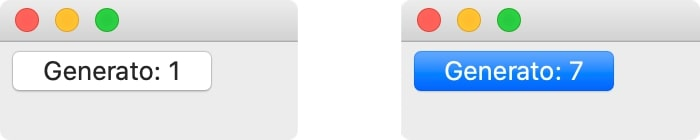
\includegraphics[width=1.0\columnwidth]{capitolo-5/qt} 
  \caption{Esempio in \emph{Qt} - Applicazione prima (sinistra) e dopo (destra) la pressione del pulsante}
\end{figure}

\subsection{Osservazioni sul procedimento}
\label{subsec:osservazioni-procedimento-qt}

Quello che si vuole evidenziare utilizzando \emph{Qt} come esempio non sono tanto le classi da usare o le necessità del linguaggio su cui si basa il \gls{frameworkg}, bensì come un'operazione di cambio dello stato dell'applicazione venga eseguita ed il ragionamento dietro ad essa.\\
Con questo tipo di \textbf{approccio imperativo}, lo sviluppatore non solo deve occuparsi dello stato dell'applicazione, ma anche dell'interfaccia grafica. Infatti nelle righe 42-43 di \texttt{ExampleApp}, una volta aggiornato $r$, lo stato, si è dovuto aggiornare il contenuto visualizzato dal pulsante tramite il metodo \texttt{setText} di \texttt{QPushButton}.

%**************************************************************
\section{Il paradigma dichiarativo: Flutter}
\label{sec:paradigma-dichiarativo-flutter}

\textbf{N.B.} L'implementazione dell'esempio è ridotta al minimo indispensabile e come si potrà vedere dalle immagini l'applicazione sarà composta da un pulsante dell'intera grandezza della schermata.

\subsection{Creazione dell'interfaccia grafica}
\label{subsec:creazione-ui-qt}

Per implementare l'esempio indicato in "\hyperref[sec:introduzione-esempio-confronto-paradigmi]{Introduzione all'esempio per il confronto}", sono necessari un po' più widget, in quanto Flutter li usa in maniera intensa, ma il codice è decisamente meno verboso.
\begin{lstlisting}
// Widget che definisce la schermata.
// Essendo uno StatefulWidget non definisce il metodo build,
// in quanto compito del possessore dello stato, ossia
// la classe _ExampleAppState.
class ExampleApp extends StatefulWidget {
  State<ExampleApp> createState() => _ExampleAppState();
}

// Stato collegato al widget ExampleApp.
class _ExampleAppState extends State<ExampleApp> {
  // Nessun widget viene dichiarato in anticipo.
  // Solo le variabili che sono parte dello stato
  // vanno dichiarate.
  final random = new Random();
  int r;
  
  // Questo metodo indica cosa va fatto ogni volta
  // che lo stato di ExampleApp viene creato da zero.
  @override
  void initState() {
    super.initState();
    r = random.nextInt(10);
  }

  // Callback che viene passata ad onPressed.
  // Corrisponde allo slot privato di ExampleApp 
  // in Qt chiamato buttonClicked.
  void _buttonClicked() {
    setState(() => r = random.nextInt(10));
  }

  // Questo metodo indica che cosa mostrare a schermo.
  // Notare come i concetti di Element e RenderObject
  // non sono presenti, in quanto sono onere di Flutter.
  @override
  Widget build(BuildContext context) {
    // MaterialApp, paragonabile a QApplication.
    return MaterialApp(
      // RaisedButton, paragonabile a QPushButton.
      home: RaisedButton(
        // In Flutter il campo dati child di un widget ha sempre 
        // tipo Widget. Quindi un pulsante non contiene solo 
        // testo, ma anche qualsiasi altra cosa (in questo
        // caso, semplice testo).
        child: Text("Generato: $r"),
        // Definizione del callback da invocare
        // alla pressione del pulsante.
        onPressed: _buttonClicked,
      ),
    );
  }
}
\end{lstlisting}
Riassumendo, nella classe \texttt{ExampleApp}, che estende \texttt{StatefulWidget}, viene:
\begin{itemize}
    \item definito il widget e siccome ha uno stato, viene creato lo stato correlato;
    \item dato che lo stato del widget interessa solo a \texttt{ExampleApp}, viene dichiarato privato (al di fuori del file non è visibile);
    \item generato il valore di $r$ iniziale in \texttt{initState};
    \item impostato nel metodo \texttt{build} che cosa viene visualizzato quando il widget viene costruito (definito $state$, \texttt{build} definisce $f(state)$);
    \item dichiarato che cosa deve avvenire all'evento di pressione del pulsante.
\end{itemize}
Quello che succede alla pressione del pulsante è la generazione di un evento \emph{onPressed} che richiama il \emph{callback} (metodo \texttt{\_buttonClicked}). All'interno del \emph{callback} ci si è occupati solo di aggiornare $r$ e di indicare che il widget va ricostruito con \texttt{setState}.

\subsection{Creazione del punto di ingresso}
\label{subsec:creazione-main-qt}

Oltre alla definizione di \texttt{ExampleApp}, va definita la funzione \texttt{main}, il punto d'ingresso del programma:
\begin{lstlisting}
import 'package:flutter/material.dart';
import 'dart:math';

void main() => runApp(ExampleApp());
\end{lstlisting}
Quello che avviene in questo \texttt{main} è inserire come widget radice nel \emph{Widget tree} un'istanza di \texttt{ExampleApp}. Visto che il \texttt{main} dispone di una sola istruzione è stato possibile usare la \emph{arrow notation}.\\
L'applicazione realizzata è la seguente:
\begin{figure}[!h] 
  \centering 
  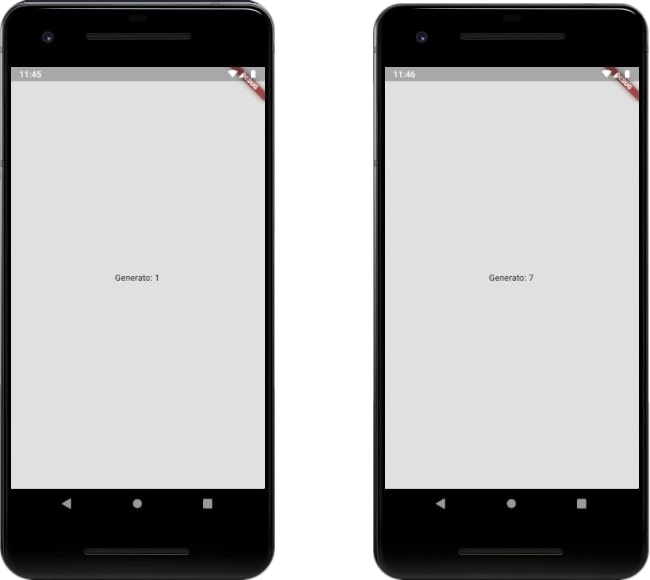
\includegraphics[width=1.0\columnwidth]{capitolo-5/flutter} 
  \caption{Esempio in Flutter - Applicazione prima (sinistra) e dopo (destra) la pressione del pulsante}
\end{figure}

\subsection{Osservazioni sul procedimento}
\label{subsec:osservazioni-procedimento-qt}

Quello che si può notare subito è la minor verbosità, sotto certi aspetti (per esempio non è necessario dichiarare che il widget va mostrato a schermo, non bisogna connettere eventi e \emph{callback} in separata sede).\\
Ma ciò che veramente conta è la separazione dei concetti.
La costruzione dell'interfaccia, basata sullo stato, è svolta solamente nel metodo \emph{build}. L'aggiornamento dello stato, svolto da \texttt{\_buttonClicked} a riga 29 di \texttt{ExampleApp}, è una pura operazione di aggiornamento stato.
Anche volendo creare un'istanza di \texttt{RaisedButton} all'esterno del metodo \texttt{build} (tecnicamente possibile) e accedendovi da dentro \texttt{\_buttonClicked}, non si sarebbe in grado di far alcuna modifica perché \texttt{RaisedButton} è un widget, e i widget sono per definizioni immutabili.
Solo richiamando \texttt{setState} è possibile informare il corrispondente \texttt{Element} che il \texttt{RenderObject} del widget va aggiornato, causando l'aggiornamento della schermata.
             % I paradigmi imperativo e dichiarativo a confronto
% !TEX encoding = UTF-8
% !TEX TS-program = pdflatex
% !TEX root = ../tesi.tex

%**************************************************************
\chapter{Dependency Injection}
\label{cap:dependency-injection}
%**************************************************************

\intro{
    In questo capitolo vengono illustrate le differenze principali fra l'implementazione della \gls{di} con due tecnologie differenti: con il \gls{frameworkg} \emph{Spring} per Java, che è stato appreso per il progetto del corso di Ingegneria del software di questo Corso di Laurea, e con \emph{Flutter}.
}\\

%**************************************************************
\section{Introduzione all'esempio per il confronto}
\label{sec:introduzione-esempio-confronto-di}

In questo capitolo l'esempio sarà molto semplificato e finalizzato a mostrare le differenze di approccio alla \gls{dig} fra i due \gls{frameworkg}.\\
Viene creata una classe che verrà usata come dipendenza da iniettare, chiamata \texttt{Dipendenza}, e una classe \texttt{Ricevente} in cui verrà iniettata la dipendenza.

%**************************************************************
\section{Inversion of Control: il framework Spring in Java}
\label{sec:ioc-spring-java}

\emph{Spring} è uno dei \gls{frameworkg} più conosciuti ed usati per sviluppare software in Java. È diviso in tanti progetti più piccoli ma che hanno tutti alla base un efficiente meccanismo di \gls{dig} attraverso l'\emph{Inversion of Control}.\\
L'\emph{Inversion of Control (talvolta abbreviato in IoC)} è un meccanismo che permette di migliorare ancora di più l'idea alla base della \gls{dig}, che consiste nel tenere il comportamento di una classe separato dalla risoluzione delle sue dipendenze, avendo un contenitore che gestisce autonomamente questo meccanismo.\\
Il compito di uno sviluppatore resta quello di dichiarare le dipendenze, dove necessarie, e registrare, attraverso dei meccanismi definiti dal \gls{frameworkg}, come permettere di ottenerle.\\
Al collegamento fra le dipendenze stesse e le classi che invece le richiedono ci pensa il meccanismo di \emph{IoC}.\\

%**************************************************************
\subsection{Creazione di una dipendenza}
\label{subsec:creazione-dipendenza-spring}

In \emph{Spring} ci sono vari modi per dichiarare al meccanismo di \emph{IoC} che un'istanza di una classe deve essere usata come dipendenza. Di seguito vengono mostrati i due principali, gli altri derivano da questi.

%**************************************************************
\subsubsection{Utilizzo di POJO: l'annotazione @Bean}
\label{subsubsec:utilizzo-pojo-annotazione-bean-spring}

Il primo modo che è disponibile per creare una dipendenza è usando l'annotazione di \emph{Spring} \texttt{@Bean}. Tipicamente questo metodo è utilizzato per ritornare oggetti singoli che vengono istanziati agevolmente all'interno di un metodo (i cosiddetti \gls{pojo}), come configurazioni di librerie o di altre parti dell'applicazione.\\
\begin{lstlisting}
class XYZ {
    ...
    @Bean
    public Dipendenza getDipendenza() {
        return new Dipendenza();
    }
}
\end{lstlisting}
Facendo riferimento all'esempio appena presentato, marchiando un'istanza o un metodo di una classe (che deve essere sotto il controllo di \emph{Spring}, nel prossimo esempio viene spiegato come) con \texttt{@Bean}, il meccanismo di \emph{IoC} si salva il riferimento all'istanza ritornata dal metodo \texttt{getDipendenza} e, quando deve istanziare un oggetto che la richiede, gliela passa come argomento.

%**************************************************************
\subsubsection{Utilizzo di classi: l'annotazione @Component}
\label{subsubsec:utilizzo-classi-annotazione-component-spring}

Un altro modo, e da questo ne derivano altri del tutto simili, è marchiare una classe con l'annotazione \texttt{@Component}.
Le differenze con gli altri sono riconducibili all'annotazione usata: \texttt{@Controller}, \texttt{@RestController}, \texttt{@Service} e \texttt{@Configuration}.
Tutte le annotazioni elencate aiutano il \gls{frameworkg} nel lavoro di risoluzione delle dipendenze, ma hanno di fondo lo stesso funzionamento.

\begin{lstlisting}
@Component
class Dipendenza {
    ...
}
\end{lstlisting}
In questo modo, quando una classe o un metodo richiedono una dipendenza di tipo \texttt{Dipendenza}, il meccanismo di \emph{IoC} crea un'istanza di questa classe e la passa come argomento.

%**************************************************************
\subsection{Richiesta di una dipendenza}
\label{subsec:richiesta-dipendenza-spring}

Il modo per informare il meccanismo di \emph{IoC} di necessitare di una dipendenza è utilizzando una delle due annotazioni \texttt{@Autowired} o \texttt{@Inject}.
\begin{lstlisting}
class Ricevente {
    @Autowired
    private Dipendenza nonDichiarata;

    private Dipendenza dichiarata;

    @Autowired
    public Ricevente(Dipendenza dipendenza) {
        dichiarata = dipendenza;
    }
}
\end{lstlisting}
In questo esempio vengono mostrati due modi per ottenere la risoluzione della dipendenza:
\begin{itemize}
    \item il primo, corrispondente alla variabile \texttt{nonDichiarata}, è ottenere la dipendenza senza dichiararla.
    È assolutamente uguale al successivo, ma non dichiarandola nel costruttore o in un setter, è più facile da dimenticare (per esempio, in fase di testing);
    \item la seconda, corrispondente alla variabile \texttt{dichiarata}, è ottenere la dipendenza dal costruttore, facendo quella che viene chiamata \emph{constructor injection}.
\end{itemize}

%**************************************************************
\subsection{Osservazioni sul procedimento}
\label{subsec:osservazioni-procedimento-spring}

Questo è quanto è necessario fare per la \gls{dig} in \emph{Spring}. Un'eccezione è fatta per il punto di ingresso, ovvero la classe con il metodo \texttt{main}, che va annotata con \texttt{@SpringBootApplication} (ma che è automaticamente incluso alla generazione di un nuovo progetto).



%**************************************************************
\section{InheritedWidget e la libreria Provider: Flutter}
\label{sec:inheritedwidget-provider}

\emph{Flutter} non ha un vero e proprio meccanismo di \emph{IoC} integrato, quindi le dipendenze vanno comunque risolte manualmente.\\
Come è stato visto, nonostante la risoluzione delle dipendenze in \emph{Spring} sia automatica, richiede comunque che esse vengano dichiarate nei costruttori delle classi.
Anche in \emph{Flutter} questo è possibile, ma può verificarsi una situazione in cui viene istanziata una dipendenza ad una certa altezza del \emph{Widget tree} e che serva ad un widget che si trovi molti livelli più in basso (e non è così difficile trovare un semplice esempio in Flutter che richieda molti widget).\\
La cosa più semplice e ovvia da fare è aggiungere un parametro al costruttore di ciascuna classe/widget che si trova nel cammino fra dove la dipendenza è dichiarata e dove viene usata.
Il problema di questo approccio è che i widget intermedi hanno un argomento con il solo scopo di passarlo al widget successivo, ma che non usano.
Inoltre, se si deve modificare la struttura del \emph{Widget tree} o se le dipendenze iniziano a crescere in numero, può crearsi molta confusione.

%**************************************************************
\subsection{Creazione di una dipendenza}
\label{subsec:creazione-dipendenza-flutter}

Per evitare questo tipo di problemi, in \emph{Flutter} è presente un tipo di widget ideato appositamente per risolvere questo tipo di problema. È diverso da \texttt{StatelessWidget} e \texttt{StatefulWidget} e si chiama \texttt{InheritedWidget} (nonostante il termine \emph{inherited} non ha nulla a che vedere con l'\emph{inheritance}, l'ereditarietà fra classi).
Questo tipo di widget non disegna nulla a schermo, è immutabile come gli altri due tipi, e permette di accedere ai suoi campi dati e metodi (pubblici) da tutti i widget suoi discendenti.
È possibile accedervi mediante il \texttt{BuildContext}, riferimento che hanno tutti i widget come argomento del metodo \texttt{build}.\\
Nonostante questa importante funzionalità, \texttt{InheritedWidget} non viene molto usato in quanto molto "primitivo" come meccanismo. Al suo posto vengono usate librerie di \gls{dig}. La più semplice, e consigliata anche nella documentazione ufficiale di \emph{Flutter}, è \emph{Provider}\footcite{site:provider}.\\
\emph{Provider} è una libreria che fa da wrapper alle funzionalità di \texttt{InheritedWidget}, e permette di crearne di vario tipo (elencati quelli conosciuti perché usati nel progetto di stage):
\begin{enumerate}
    \item \texttt{Provider} permette di istanziare una dipendenza di qualsiasi tipo, che non dipende da altre disponibili via \texttt{InheritedWidget};
    \item \texttt{ProxyProvider} è come il precedente, ma può permettere la dichiarazione di dipendenze in ingresso necessarie per la sua creazione e che sono rese disponibili tramite \texttt{InheritedWidget};
    \item \texttt{ChangeNotifierProvider} è come il primo, ma la dipendenza implementa, estende o usa come mixin \texttt{ChangeNotifier} (che permette di utilizzare il \gls{designpatterng} Observer);
    \item \texttt{ChangeNotifierProxyProvider} come il secondo, ma nuovamente la dipendenza dispone di \texttt{ChangeNotifier}.
\end{enumerate}
Il secondo e il quarto tipo di \texttt{Provider} sono disponibili in più versioni, che accettano da 0 fino a 6 dipendenze in ingresso.\\
L'esempio mostra come utilizzare la libreria:
\begin{lstlisting}
class XYZ extends StatelessWidget {
  @override
  Widget build(BuildContext context) {
    return Provider(
      create: (context) => Dipendenza(),
      child: ...,
    );
  }
}
\end{lstlisting}
La dipendenza viene istanziata dal \emph{callback} presente in \texttt{create}. Di default, se non specificato il parametro \texttt{lazy} (di tipo \texttt{bool}), la dipendenza viene istanziata solo se fra i discendenti del widget ce n'è uno che lo richiede (a fini di efficienza).

%**************************************************************
\subsection{Richiesta di una dipendenza}
\label{subsec:richiesta-dipendenza-flutter}

Per richiedere una dipendenza sono disponibili due modalità: la prima richiede l'utilizzo di un metodo statico della classe \texttt{Provider}, la seconda un widget chiamato \texttt{Consumer}.

%**************************************************************
\subsubsection{Utilizzo di un metodo statico: Provider.of}
\label{subsubsec:utilizzo-metodo-statico-providerof-flutter}

Questo tipo di modalità è quella che ricalca maggiormente l'originale utilizzo di \texttt{InheritedWidget}.\\
Dove è necessario accedere alla dipendenza, si utilizza il metodo che ha come firma completa \texttt{T of<T>(BuildContext context)}.
La \texttt{T} indica un tipo generico, quello che in Java si chiamerebbe \emph{generic} e in C++ \emph{template}, e questo si riferisce al tipo della dipendenza richiesta.

\begin{lstlisting}
// Ricevente deve essere discendente del widget XYZ,
// altrimenti non permette di accedere a Dipendenza.
class ABC extends StatelessWidget {
  @override
  Widget build(BuildContext context) {
    return Ricevente(
      dipendenza: Provider.of<Dipendenza>(context),
      child: ...,
    );
  }
}
\end{lstlisting}
In questo caso il widget \texttt{Ricevente} riceve la dipendenza richiesta.
\texttt{Dipendenza} può essere stata creata con uno qualsiasi dei tipi di \texttt{Provider} presentati sopra, quindi può capitare che \texttt{Dipendenza} si aggiorni o invii notifiche mediante \texttt{ChangeNotifier}:
\begin{itemize}
    \item se si vuole che un cambiamento venga riflesso sull'interfaccia grafica, è sufficiente quanto scritto nell'esempio;
    \item se invece non si vuole che l'interfaccia grafica si aggiorni di conseguenza, va usata l'istruzione \texttt{Provider.of<Dipendenza>(context, listen: false)}.
\end{itemize}
Come si può evincere dall'esempio mostrato, il parametro \texttt{listen} è implicitamente \texttt{true}.

%**************************************************************
\subsubsection{Utilizzo di un widget: Consumer}
\label{subsubsec:utilizzo-widget-consumer-flutter}

Questa modalità è assolutamente equivalente alla precedente con \texttt{listen} non impostato.\\
È usabile in qualsiasi caso in cui è necessario ricostruire l'interfaccia sempre e comunque, ma necessario in altri casi particolari:
\begin{enumerate}
    \item la dipendenza è necessaria nel primo discendente del \texttt{Provider}, in cui si ha lo stesso \texttt{BuildContext};
    \item non si vuole che l'intera porzione di \emph{Widget tree} in cui si è venga ricostruita.
\end{enumerate}
Il caso descritto nell'esempio 1 è il seguente:
\begin{lstlisting}
class XYZ extends StatelessWidget {
  @override
  Widget build(BuildContext context) {
    return Provider(
      create: (context) => Dipendenza(),
      child: Ricevente(
        dipendenza: Provider.of<Dipendenza>(context),
        child: ...,
      );
    );
  }
}
\end{lstlisting}
Il problema è risolvibile sostituendo la dichiarazione di \texttt{Ricevente} con questo:
\begin{lstlisting}
Consumer<Dipendenza>(
  builder: (context, dipendenza, noRebuild) => Ricevente(
    dipendenza: dipendenza,
    child: ...
  ),
  child: ...
)
\end{lstlisting}
Con \texttt{Consumer} si può dichiarare, usando la proprietà \texttt{child}, un widget (e quindi, per ricorsività, anch'esso un \emph{Widget tree}) che quando \texttt{dipendenza} si aggiorna non richiede il rebuild.
Per utilizzarlo nella parte di \emph{Widget tree} radicata in \texttt{Ricevente} basta utilizzare l'argomento \texttt{noRebuild} di \texttt{builder}.\\\\
Il caso dell'esempio 2 è più fine:
\begin{lstlisting}
class ABC extends StatelessWidget {
  @override
  Widget build(BuildContext context) {
    return WidgetCostoso(
      child: Ricevente(
        dipendenza: Provider.of<Dipendenza>(context),
        child: ...,
      ),
    );
  }
}
\end{lstlisting}
In questo caso, molto simile a quello della spiegazione di \texttt{Provider.of}, se \texttt{Dipendenza} viene aggiornata viene rilanciato il metodo \texttt{build} di \texttt{ABC} e non solo quello di \texttt{Ricevente} (con la conseguenza di rieseguire \texttt{build} anche di \texttt{WidgetCostoso}).\\
Il problema è ovviabile come per l'esempio 1.

%**************************************************************
\subsection{Osservazioni sul procedimento}
\label{subsec:osservazioni-procedimento-flutter}

Questo è tutto ciò che c'è da fare per la \gls{dig} in \emph{Flutter}. L'\emph{IoC} o altri tipi di \gls{dig} diversi dall'uso di \texttt{InheritedWidget} non sono ancora implementati per decisione degli sviluppatori.\\
Altri metodi che non richiedono \emph{InheritedWidget} sono disponibili: essi registrano le dipendenze all'interno di un contenitore in memoria e permettono di accedervi attraverso metodi statici. Nessuno di questi è citato o consigliato fortemente quanto \emph{Provider} nella documentazione ufficiale e per questo motivo si è evitato di utilizzarli.             % Dependency Injection
% !TEX encoding = UTF-8
% !TEX TS-program = pdflatex
% !TEX root = ../tesi.tex

%**************************************************************
\chapter{Prodotto dello stage}
\label{cap:prodotto-stage}
%**************************************************************

\intro{
    In questo capitolo viene presentato il processo decisionale che ha portato alla scelta dell'architettura software alla base del prodotto realizzato e quali erano state considerate per svolgere lo stesso scopo. Viene quindi presentata l'organizzazione del \gls{codebaseg} e la sua suddivisione in package, spiegando di ciascuno di questi il significato. Si entra poi in dettaglio di come il pattern Observer è stato fondamentale per lo sviluppo di un'architettura ben organizzata e con compiti precisi. Infine, viene fatto un confronto fra l'applicazione in uso presso l'azienda e quella sviluppata per lo stage, riflettendo sulle modifiche apportate.
}

%**************************************************************
\section{Architetture a confronto}
\label{sec:architetture-confronto}

Prima di procedere con la progettazione delle componenti in dettaglio e della vista si sono analizzati più \gls{designpatterng} architetturali per capire quale fosse il più adeguato per lo scopo.\\
La scelta è stata influenzata da fattori come la facilità di implementazione, la facilità di adattamento a \emph{Flutter} e di conseguenza la disponibilità di esempi.\\
Mentre per sviluppare un'applicazione nativa in Android è consigliato usare l'architettura Model View Presenter e in \emph{Qt} quella Model View (una versione modificata di Model View Controller), per Flutter non c'è ancora una \gls{bestpracticeg} diffusa.

%**************************************************************
\subsection{Model View Controller}
\label{subsec:model-view-controller}

Il \emph{Model View Controller (MVC)} è un tipo di architettura molto famosa e molto implementata, ma spesso in maniera errata.\\
Permette di avere, nel proprio sistema, tre componenti che hanno compiti distinti (e lo stesso vale per le altre architetture).\\
In MVC:
\begin{itemize}
    \item il \emph{Model} rappresenta il modello dei dati, ovvero tutto ciò che implementa la \emph{business logic}, comprese le operazioni sui dati (lettura e scrittura da supporti di persistenza e da remoto). Quando viene aggiornato, si occupa di notificare la \emph{View} (tramite il \gls{designpatterng} Observer\footnote{Per maggiori informazioni su Observer, consultare alla sotto-sezione "\hyperref[subsec:observer-provider-changenotifier]{Il design pattern Observer: Provider, ChangeNotifier e Consumer}".});
    \item la \emph{View} rappresenta la parte di \emph{presentation logic}, ovvero ciò che permette di interagire con l'utente. Gli input dell'utente vengono catturati e inoltrati al \emph{Controller};
    \item il \emph{Controller} rappresenta la parte di \emph{application logic} poiché seleziona la \emph{View} corretta in base all'input e inoltra i dati dell'interazione dell'utente al \emph{Model}.
\end{itemize}
Questa architettura è facilmente applicabile in \emph{Flutter}, poiché la vista è correttamente separata dal modello e si gestisce autonomamente il proprio aggiornamento (ad eccezione della selezione che la fa il \emph{Controller}).\\
Sebbene siano separati, la dipendenza della vista dal modello non li rende completamente separati per cui il modello, dovendo fornire metodi per le richieste provenienti dalla vista, dovrebbe già preparare i dati in un formato adeguato, rendendolo più complesso.

\begin{figure}[!h]
    \centering 
    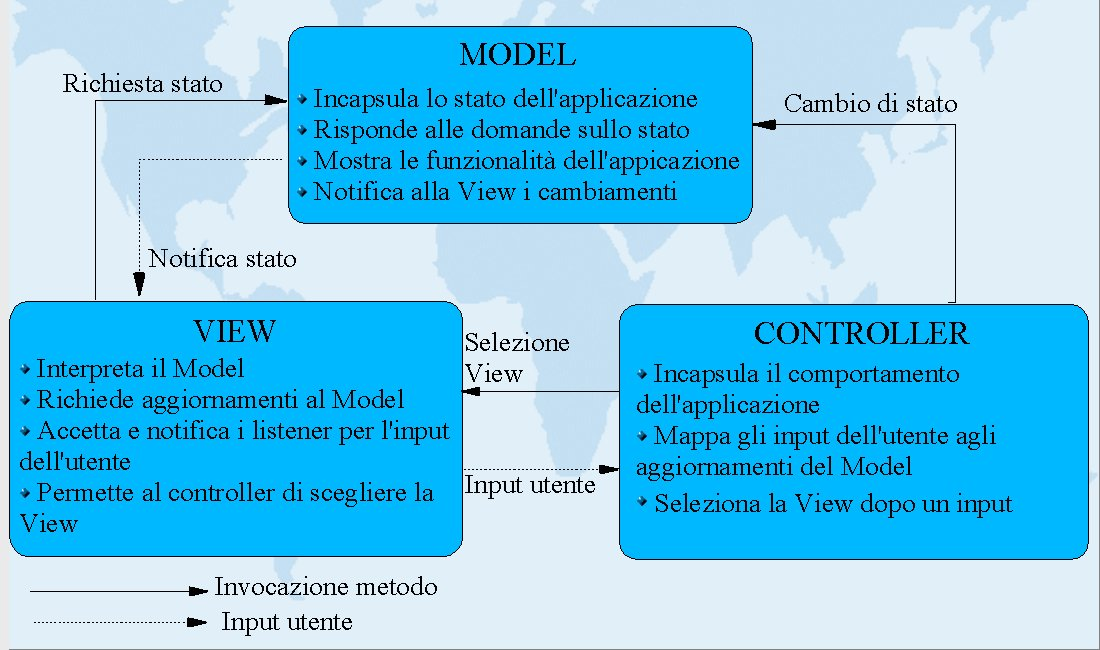
\includegraphics[width=0.9\columnwidth]{capitolo-6/architetture-confrontro/mvc} 
    \caption{Diagramma dell'architettura MVC (da \cite{site:mvc})}
\end{figure}

%**************************************************************
\subsection{Model View Presenter}
\label{subsec:model-view-presenter}

Il \emph{Model View Presenter (MVP)} è invece un'architettura in cui il modello e la vista sono due entità completamente separate e fra di loro sconosciute.\\
Più in dettaglio:
\begin{itemize}
    \item il \emph{Model} rappresenta il modello dei dati, ovvero tutto ciò che implementa la \emph{business logic}, comprese le operazioni sui dati (lettura e scrittura da supporti di persistenza e da remoto). Non notifica la \emph{View} in caso di aggiornamento, ma chiama il \emph{Presenter};
    \item la \emph{View} rappresenta la pura interfaccia di visualizzazione per l'utente (è passiva) oppure può anche contattare il \emph{Presenter} in caso di eventi, in base all'implementazione;
    \item il \emph{Presenter} agisce da "Man in the middle" poiché fa da passacarte fra la \emph{View} e il \emph{Model}. A meno che non sia la \emph{View} stessa a chiamarlo, resta in ascolto di notifiche da parte di entrambi e aggiorna lo stato dell'applicazione o della vista in base alle necessità.
\end{itemize}
Con questo approccio c'è una separazione dei compiti importante ma è richiesto che il \emph{Presenter} si occupi dell'aggiornamento della vista, rendendolo poco adatto a \emph{Flutter}.

\begin{figure}[!h]
    \centering 
    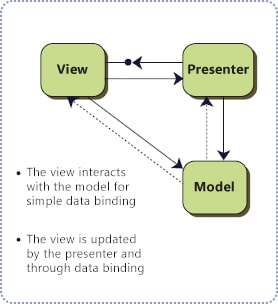
\includegraphics[width=0.5\columnwidth]{capitolo-6/architetture-confrontro/mvp} 
    \caption{Diagramma dell'architettura MVP (da \cite{site:mvp})}
\end{figure}

%**************************************************************
\subsection{Model View ViewModel}
\label{subsec:model-view-viewmodel}

Il \emph{Model View ViewModel (MVVM)} è un'architettura che consente di separare il modello e la vista utilizzando un doppio Observer.\\
Più specificatamente:
\begin{itemize}
    \item il \emph{Model} è il medesimo dell'architettura MVP;
    \item la \emph{View} è la medesima dell'architettura MVC, ma chiaramente in caso di input viene contattato un \emph{ViewModel} e non un \emph{Controller};
    \item il \emph{ViewModel} è il "modello della vista", ovvero il \emph{Model} accinge solo da questo, che accinge a sua volta solo dal \emph{Model}.
\end{itemize}
In MVVM, la \emph{View} è spesso implementata dichiarativamente (e questo è un punto a favore per \emph{Flutter}).\\
Come è stato detto, la \emph{View} può sfruttare il proprio \emph{ViewModel} per ottenere i dati da visualizzare e il \emph{ViewModel} a sua volta utilizza il proprio \emph{Model}.
Essendo implementato il \gls{designpatterng} Observer, quando il \emph{Model} e il \emph{ViewModel} hanno nuovi dati notificano i propri listener (che sono rispettivamente delle \emph{View} e dei \emph{ViewModel}), senza sapere chi è il destinatario.\\

\begin{figure}[!h]
    \centering 
    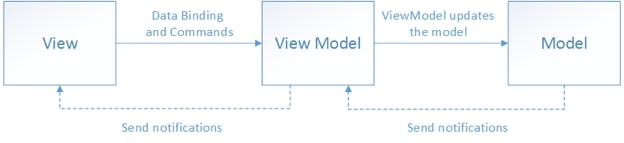
\includegraphics[width=0.7\columnwidth]{capitolo-6/architetture-confrontro/mvvm} 
    \caption{Diagramma dell'architettura MVVM (da \cite{site:mvvm})}
\end{figure}

%**************************************************************
\subsection{Clean Architecture}
\label{subsec:clean-architecture}

La \emph{Clean Architecture} si differenza molto dalle altre tre perché si concentra su una cosa fondamentale: le \textbf{dipendenze} e come \textbf{minimizzarle}.\\
In questo tipo di architettura le dipendenze vanno solo in un verso, che nel diagramma dell'architettura corrisponde dall'esterno all'interno degli strati del cerchio.\\
Più in dettaglio, questa architettura si compone di quattro macro-livelli:
\begin{itemize}
    \item \emph{Entities}, che sono entità gestite da regole di business (per esempio i prodotti gestiti da un'azienda), potenzialmente riusabili in più applicazioni dell'organizzazione, e che hanno meno probabilità di cambiare se cambia il funzionamento del sistema;
    \item \emph{Use cases}, che gestiscono la \emph{business logic} dell'applicazione seguendo i casi d'uso specifici. Ha dipendenze solo verso il livello \emph{Entities} ed è isolato dal resto (modifiche a livelli sovrastanti non ne richiedono la modifica);
    \item \emph{Interface adapters}, che contiene tutti gli adattatori (tra cui i già citati \emph{Controller}, \emph{Presenter}) fra le regole di business (livello \emph{Use cases}) e i dati provenienti da interfacce utente, remoto, file, database (livello \emph{Frameworks and Drivers});
    \item \emph{Frameworks and Drivers} contiene infine tutto il codice che dipende da implementazioni di altro software come appunto database, \gls{api} di librerie o in rete. Questo livello contiene tutti i "\textbf{dettagli}" (implementativi).
\end{itemize}
È un architettura sicuramente molto valida e che può garantire una forte separazione delle responsabilità, fondamentale per avere un \gls{codebaseg} mantenibile e scalabile, ma difficile da padroneggiare per un novizio (richiede come minimo una buona conoscenza delle regole di business, cosa che in uno stage non è presente).

\begin{figure}[!h]
    \centering 
    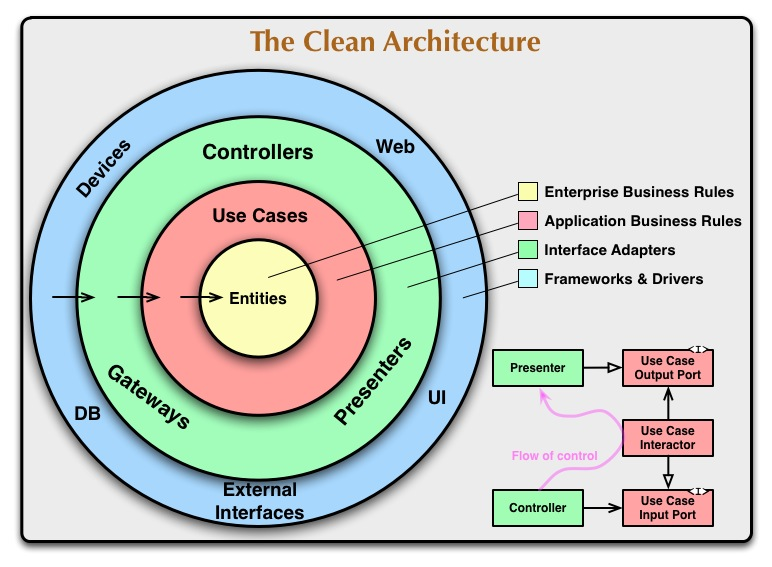
\includegraphics[width=0.8\columnwidth]{capitolo-6/architetture-confrontro/clean-architecture} 
    \caption{Diagramma dell'architettura Clean Architecture (da \cite{site:clean-architecture})}
\end{figure}

%**************************************************************
\section{Model View ViewModel, l'architettura scelta}
\label{sec:architettura-mvvm}

%**************************************************************
\subsection{Ragioni della scelta}
\label{subsec:ragioni-scelta}

Dopo aver analizzato le varie caratteristiche delle architetture presentate nella precedente sezione, è stata scelta l'architettura \emph{Model View ViewModel}.\\
Innanzitutto, \emph{MVVM} è consigliato per alcune delle altre tecnologie multipiattaforma che sono state ipotizzate per realizzare il prodotto di stage, per via della natura dichiarativa con cui viene implementata l'interfaccia utente.
Inoltre, l'utilizzo del \gls{designpatterng} Observer doppiamente permette di garantire un notevole disaccoppiamento fra le tre parti dell'architettura, permettendo di conseguenza una maggior facilità nel testing.\\
Per quanto riguarda le altre architetture, \emph{Model View Presenter} è stata scartata principalmente per la necessità del \emph{Presenter} di aggiornare la vista, che non si trova molto in sintonia con il metodo di rappresentazione dell'interfaccia di \emph{Flutter}.\\
\emph{Model View Controller} non è stato scelto perché il \emph{Model} avrebbe avuto troppi oneri: nel sistema da realizzare per lo stage era necessario memorizzare i dati ottenuti dalle \gls{restg} per poterli utilizzare per più scopi in più viste, quindi richiedendo che in qualche punto dell'architettura ci sia questo tipo di disponibilità (possibilmente non nella \emph{View}).\\
Infine, \emph{Clean Architecture}, come affermato nella sotto-sezione in cui la si illustrava, è certamente una buona architettura ma difficilmente implementabile con l'esperienza avuta fino ad ora. È comunque un'architettura valida e con i dovuti aggiustamenti \emph{MVVM} potrebbe essere adattata a questa.

%**************************************************************
\subsection{Organizzazione dei package}
\label{subsec:organizzazione-package}

%**************************************************************
\subsubsection{Package it.tecsen.smacs}
\label{subsubsec:it-tecsen-smacs}

\begin{figure}[!h] 
  \centering 
  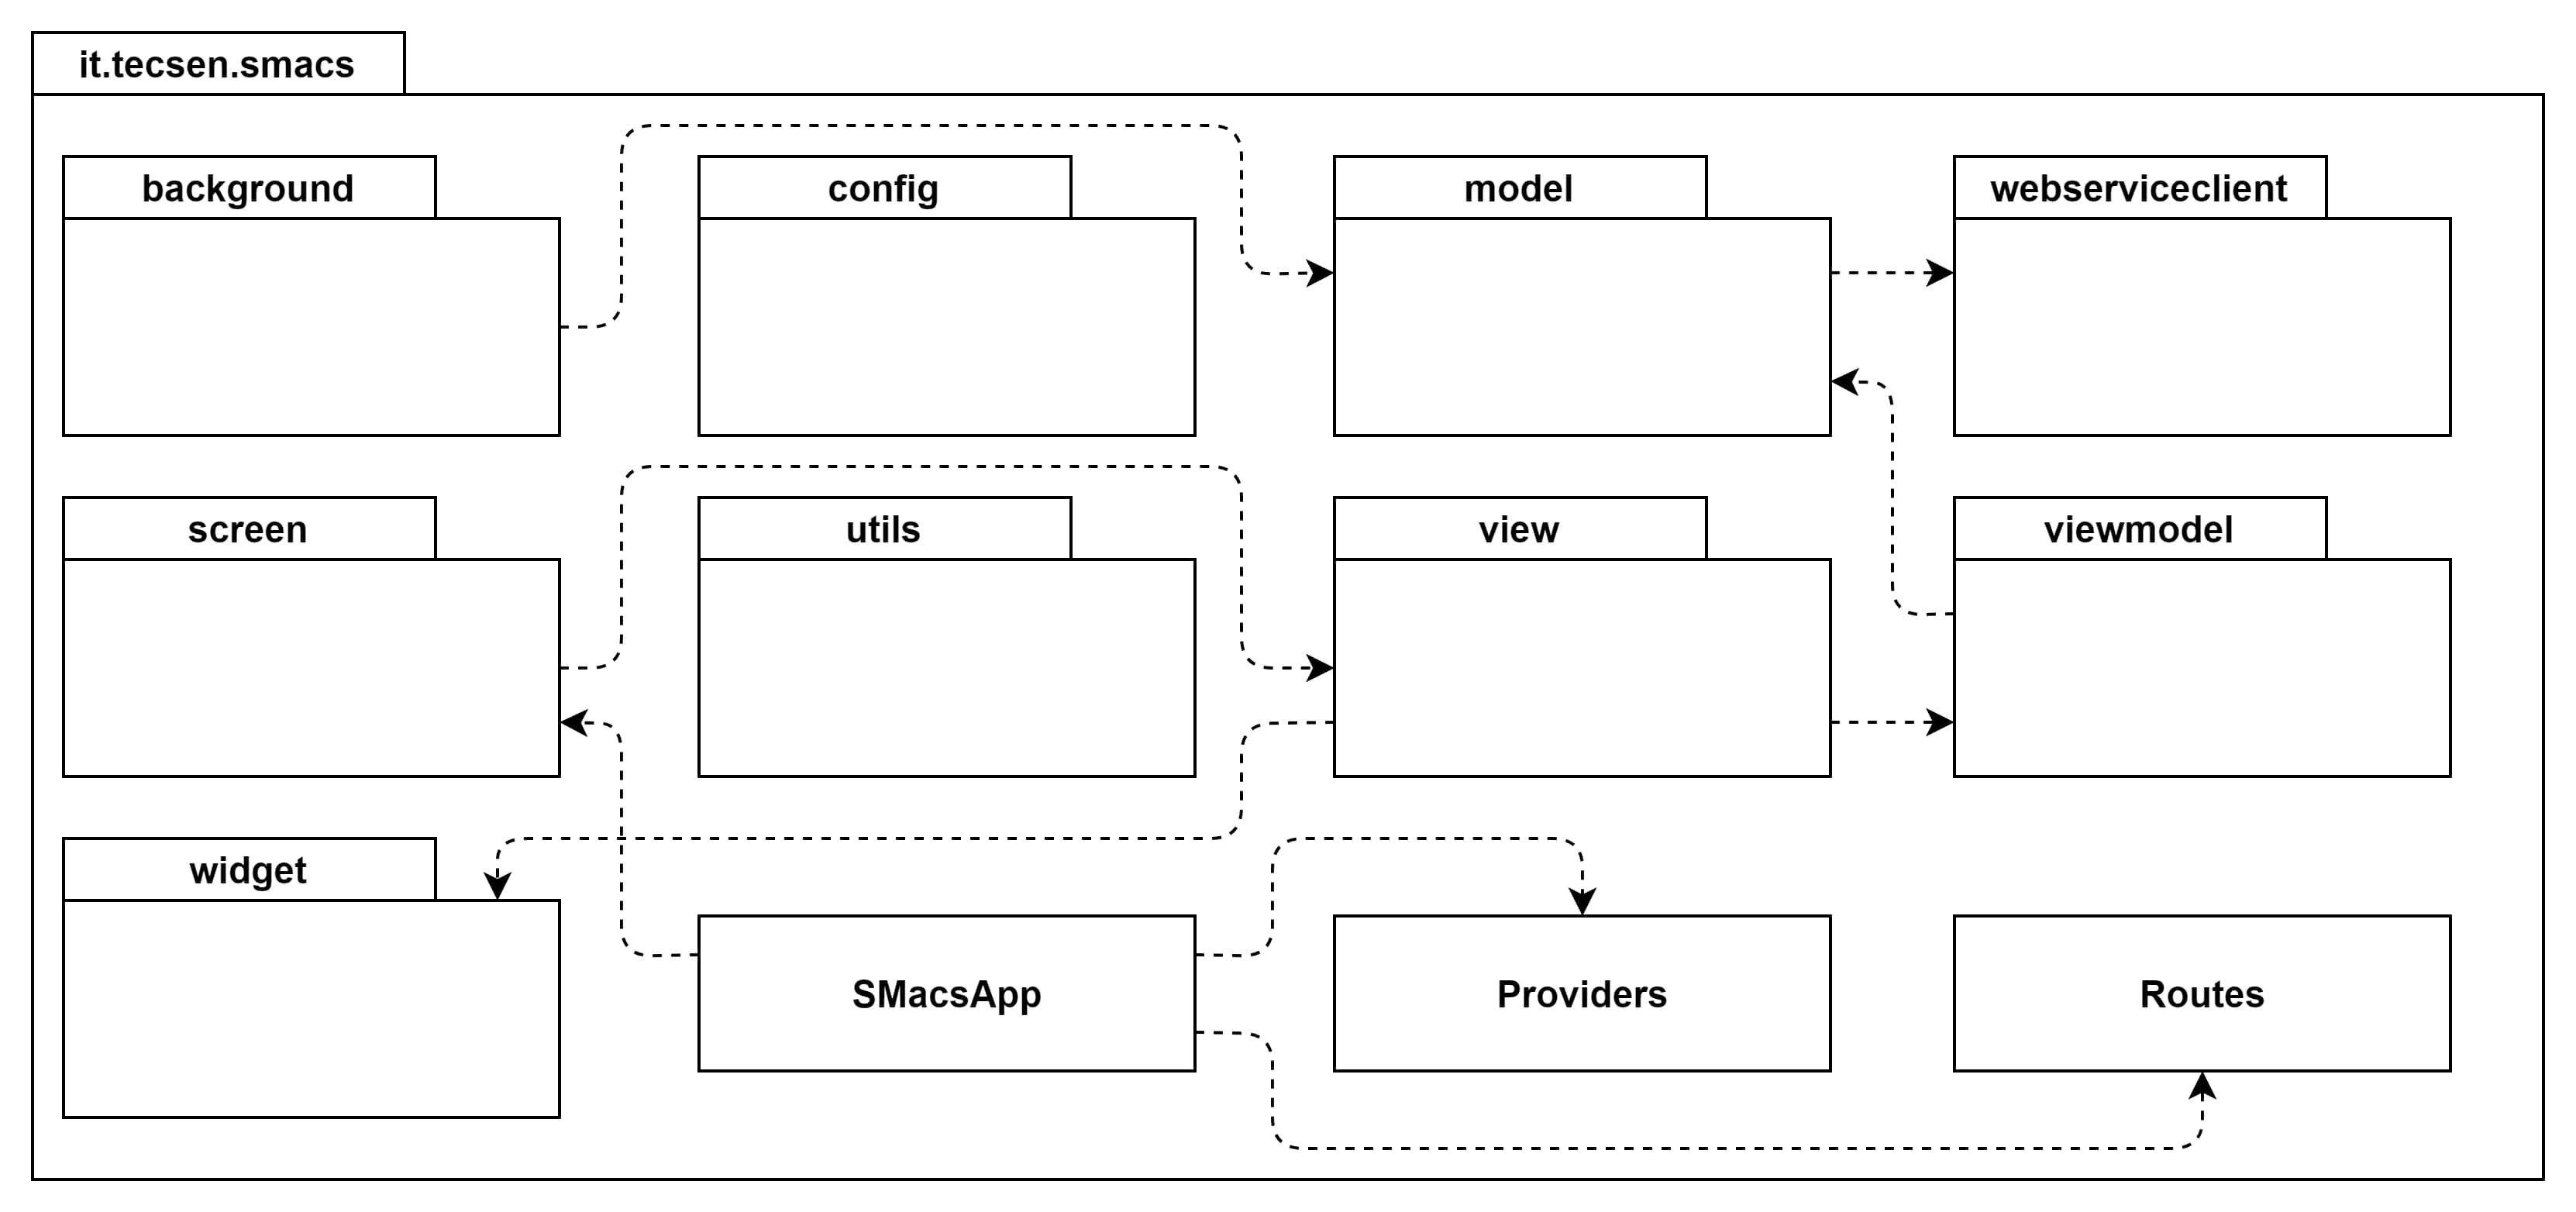
\includegraphics[width=1.0\columnwidth]{capitolo-6/organizzazione-package/it-tecsen-smacs} 
  \caption{Diagramma del package \texttt{it.tecsen.smacs}}
\end{figure}
Il seguente package racchiude tutto il codice sorgente dell'applicazione (non è stato richiesto l'uso del \emph{Platform Channel}), librerie escluse.\\
È suddiviso in più sotto-package seguendo il pattern architetturale Model View ViewModel, per cui sono presenti (come si può vedere nel diagramma sottostante) i package \texttt{model}, \texttt{viewmodel} e \texttt{view}.\\
\textbf{N.B.} Le dipendenze evidenziate nel diagramma sono quelle principali. Ad esempio, quasi tutti i package dipendono da \texttt{utils} e \texttt{config}, dato che contengono rispettivamente classi di utilità e di configurazione, ma non sono state segnate.\\
I package \texttt{screen} e \texttt{widget} fanno sempre parte del concetto \texttt{view} del pattern, ma sono separate dal package \emph{view} per ragioni organizzative:
\begin{itemize}
  \item \texttt{screen} contiene le classi che implementano i widget radice di ogni schermata dell'applicazione. Ognuno di questi widget è ridotto al minimo essenziale per poter poi utilizzare un widget dichiarato nel package \texttt{view} come resto del \emph{Widget tree};
  \item \texttt{widget} contiene le classi che implementano alcuni widget usati dalle classi in \texttt{screen} e \texttt{view}, a scopo di riutilizzo.
\end{itemize}
I package \texttt{model}, \texttt{viewmodel} e \texttt{view} contengono le classi per svolgere il loro ruolo all'interno dell'architettura.\\
Il package \texttt{utils} contiene classi con metodi di utilità (per esempio per il parsing di UUID, per l'hashing di stringhe, per la gestione di date, del logging e altro).\\
Il package \texttt{config} contiene classi con la configurazione dell'app, di alcuni plugin (come quello per la pubblicazione di notifiche), dell'internazionalizzazione e mappe per analizzare i dati ricevuti dalle \gls{restg}.\\
Il package \texttt{webserviceclient} contiene l'implementazione di un semplice wrapper di alcuni metodi della libreria \emph{http}\footcite{site:http-library} per facilitarne l'uso all'interno delle classi del package \texttt{model}.\\
Infine, \texttt{SMacsApp} è la classe che implementa il widget radice dell'intera applicazione e si serve delle classi \texttt{Routes} e \texttt{Providers} in cui sono presenti rispettivamente la configurazione della navigazione all'interno dell'app e le dipendenze di tutte le classi del package \texttt{viewmodel}.


%**************************************************************
\subsubsection{Package it.tecsen.smacs.screen}
\label{subsubsec:it-tecsen-smacs-screen}

% L'immagine dovrebbe essere qui ma per motivi di spazio viene spostata.
In questo package vi sono tutte le classi che implementano i widget radice di ogni schermata dell'applicazione, come è stato precedentemente illustrato in "\hyperref[subsubsec:it-tecsen-smacs]{Package it.tecsen.smacs}".\\
Ogni screen implementa uno o più casi d'uso, disponibili per la consultazione nell'appendice "\hyperref[cap:analisi-dei-requisiti]{Analisi dei requisiti}".
% \\
\clearpage
\begin{figure}[!h]
  \centering 
  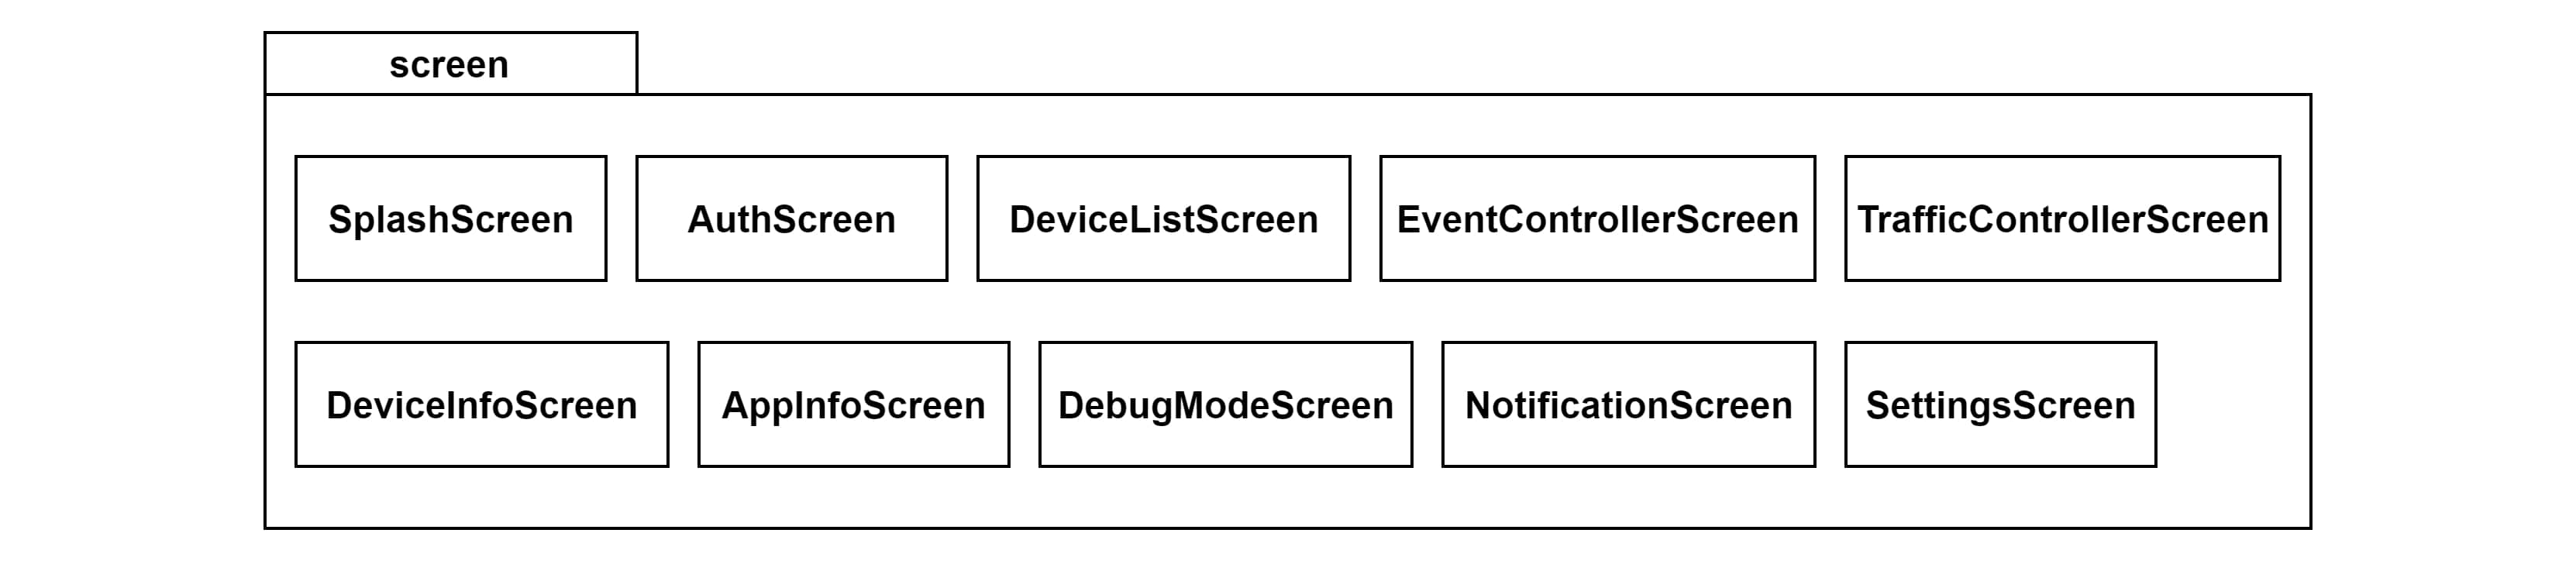
\includegraphics[width=1.0\columnwidth]{capitolo-6/organizzazione-package/screen} 
  \caption{Diagramma del package \texttt{it.tecsen.smacs.screen}}
\end{figure}
In particolare:
{
\renewcommand{\arraystretch}{1.5}
\begin{longtable}{|c|c|}
    \hline
    \textbf{Classe (widget)} & \textbf{Caso (e sotto-casi) d'uso implementati} \\\hline
    \endhead
    SplashScreen & UC01\\\hline
    AuthScreen & UC02 \\\hline
    DeviceListScreen & UC03, UC15 \\\hline
    TrafficControllerScreen & UC04, UC05, UC07, UC09, UC10 \\\hline
    DeviceInfoScreen & UC06 \\\hline
    EventControllerScreen & UC08 \\\hline
    NotificationScreen & UC11 \\\hline
    SettingsScreen & UC12 \\\hline
    AppInfoScreen & UC13 \\\hline
    DebugModeScreen & UC14 \\\hline
    \caption{Correlazione fra classi del package \texttt{screen} e casi d'uso implementati}
\end{longtable}
}


%**************************************************************
\subsubsection{Package it.tecsen.smacs.view}
\label{subsubsec:it-tecsen-smacs-view}

\begin{figure}[!h]
  \centering 
  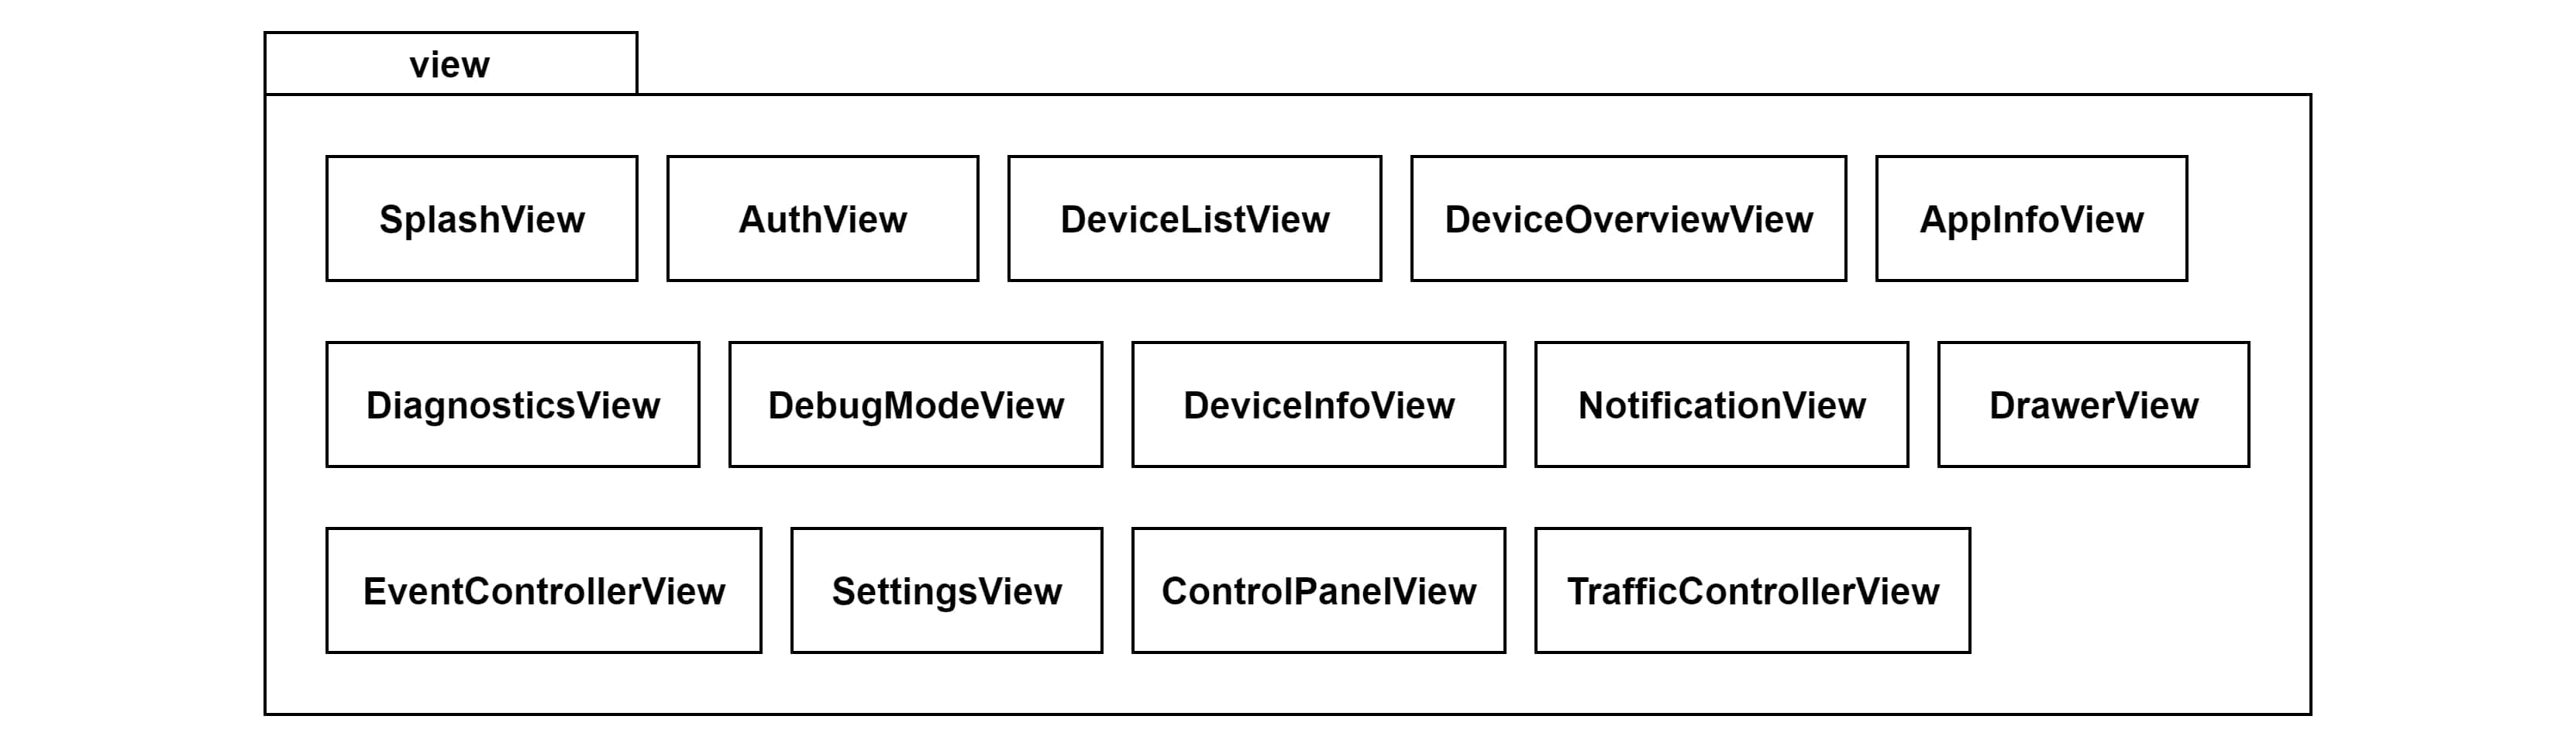
\includegraphics[width=1.0\columnwidth]{capitolo-6/organizzazione-package/view} 
  \caption{Diagramma del package \texttt{it.tecsen.smacs.view}}
\end{figure}
In questo package vi sono tutte le classi che implementano i widget che visualizzano il contenuto per soddisfare i casi d'uso raccolti.\\
Ogni classe implementa uno o più casi d'uso, disponibili per la consultazione nell'appendice "\hyperref[cap:analisi-dei-requisiti]{Analisi dei requisiti}".\\
In particolare:
{
\renewcommand{\arraystretch}{1.5}
\begin{longtable}{|c|c|}
    \hline
    \textbf{Classe (widget)} & \textbf{Caso (e sotto-casi) d'uso implementati} \\\hline
    \endhead
    SplashView & UC01\\\hline
    AuthView & UC02 \\\hline
    DeviceListView & UC03 \\\hline
    DeviceOverviewView & UC04.1, UC04.2, UC04.3, UC04.4, UC04.5, UC05 \\\hline
    DiagnosticsView & UC04.5, UC04.6, UC07.3 \\\hline
    ControlPanelView & UC04.5, UC07.1, UC07.2, UC07.4 \\\hline
    TrafficControllerView & UC04 e UC07 (sotto-casi esclusi), UC04.7, UC09, UC10 \\\hline
    DeviceInfoView & UC06 \\\hline
    EventControllerView & UC08 \\\hline
    NotificationView & UC11 \\\hline
    SettingsView & UC12 \\\hline
    AppInfoView & UC13 \\\hline
    DebugModeView & UC14 \\\hline
    DrawerView & UC15 \\\hline
    \caption{Correlazione fra classi del package \texttt{view} e casi d'uso implementati}
\end{longtable}
}

%**************************************************************
\subsubsection{Package it.tecsen.smacs.viewmodel}
\label{subsubsec:it-tecsen-smacs-viewmodel}

\begin{figure}[!h]
  \centering 
  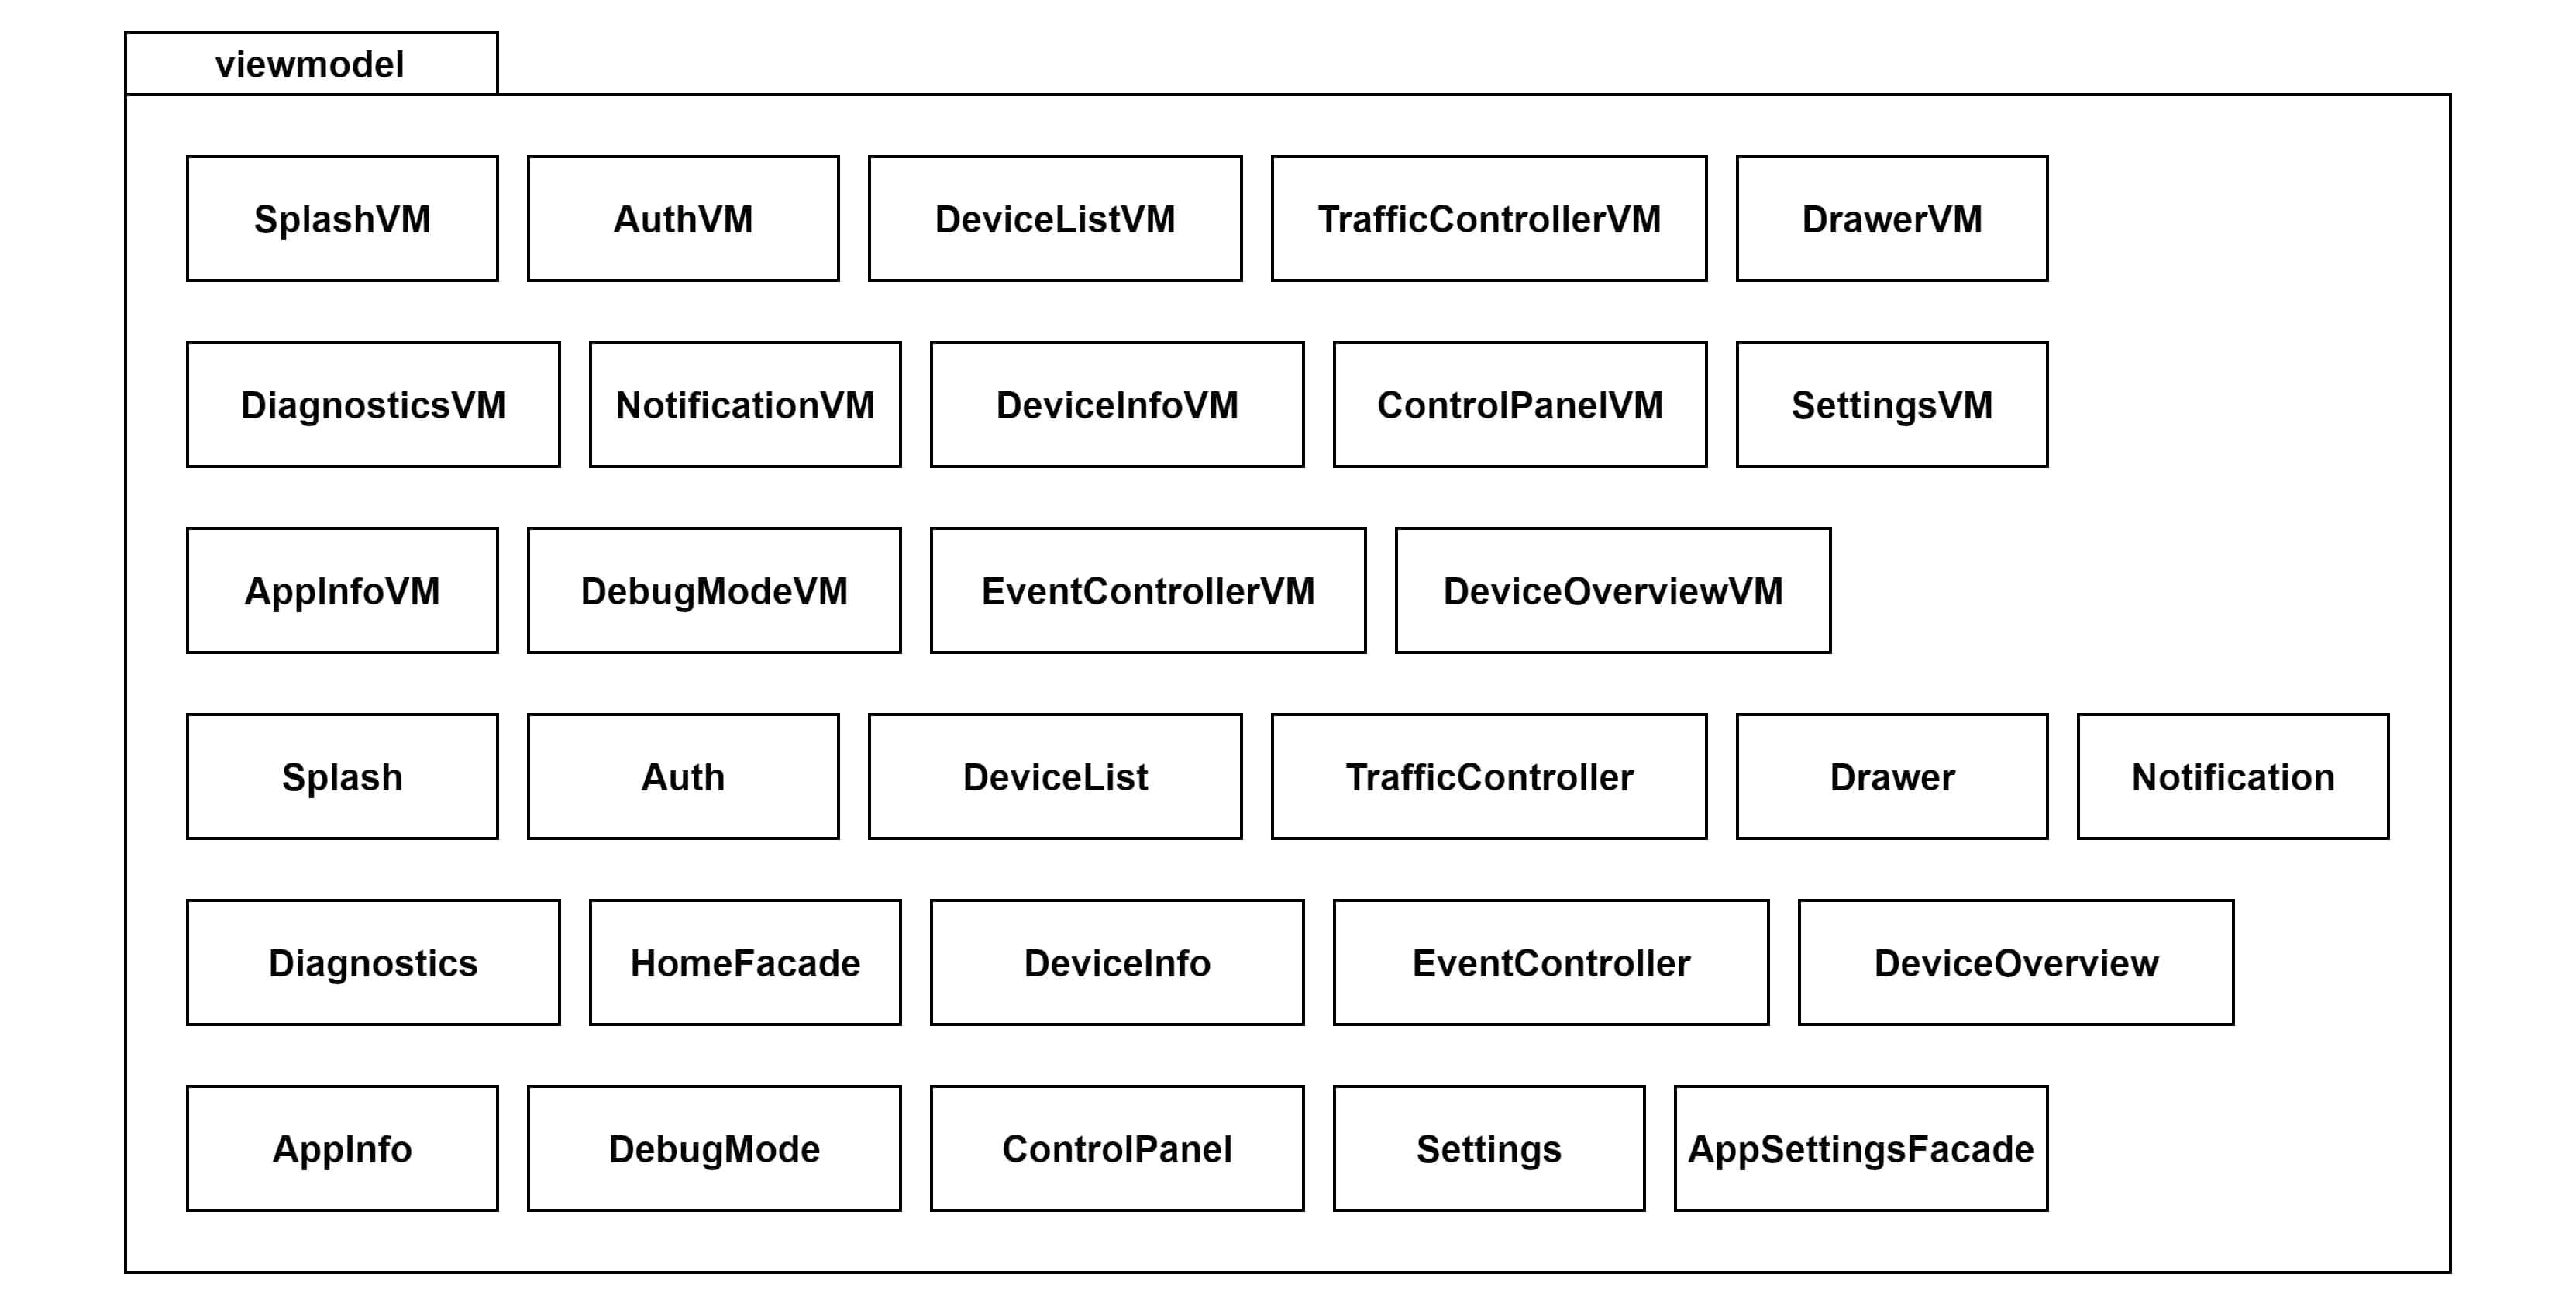
\includegraphics[width=1.0\columnwidth]{capitolo-6/organizzazione-package/viewmodel} 
  \caption{Diagramma del package \texttt{it.tecsen.smacs.viewmodel}}
\end{figure}
In questo package vi sono tutte le classi che implementano i viewmodel (ossia i model per le view) che permettono alle classi del package \texttt{view} di mostrare agevolmente i dati a schermo.\\
Per ogni viewmodel esiste un'interfaccia\footnote{Da qui in avanti in questa sezione, quando si utilizza il termine "interfaccia", si intende una classe astratta con tutti metodi astratti. Viene usato quindi il significato tipico di Java e non quello di Dart.} (tutte le classi che terminano con VM) e un'implementazione (le altre rimanenti).\\
Le classi \texttt{HomeFacade} e \texttt{AppSettingsFacade} non sono implementazioni di interfacce. Entrambi, come suggerisce il loro nome (\emph{facade}), sono classi che implementano l'omonimo \gls{designpatterng} per raggruppare funzionalità comuni necessarie alle classi del package \texttt{view}.
Il primo implementa funzionalità comuni per \texttt{SplashView} e \texttt{AuthView}. Il secondo contiene metodi e proprietà per la gestione delle impostazioni dell'applicazione, tra cui la presenza o meno di notifiche, lo stato del task in background e la durata del suo timeout di accensione.\\
Ogni interfaccia di questo package viene usata da una sola classe del package \texttt{view}, e queste non hanno accesso all'implementazione concreta. I \emph{facade} vengono invece usati in più classi dello stesso package.


%**************************************************************
\subsubsection{Package it.tecsen.smacs.utils}
\label{subsubsec:it-tecsen-smacs-utils}

\begin{figure}[!h]
  \centering 
  
\includegraphics[width=1.0\columnwidth]{capitolo-6/organizzazione-package/utils} 
  \caption{Diagramma del package \texttt{it.tecsen.smacs.utils}}
\end{figure}
In questi package ci sono strumenti di utilità creati per evitare di duplicare quanto più possibile codice.\\
Ogni classe ha il suo scopo, riassunto di seguito:
\begin{itemize}
  \item \texttt{CryptoUtils} include metodi per la cifratura di stringhe;
  \item \texttt{DateUtils} include metodi per ottenere date formattate in più modi;
  \item \texttt{FileIO} è un \emph{mixin} che viene utilizzato per memorizzare su file alcuni dati dell'applicazione dalle classi del package \texttt{it.tecsen.smacs.model.repository};
  \item \texttt{UuidUtils} include metodi per la codifica e la decodifica di \gls{uuid};
  \item \texttt{FutureUtils} include metodi per l'esecuzione sicura di funzioni che ritornano istanze di tipo \texttt{Future};
  \item \texttt{SynopticUtils} include metodi per la codifica e la decodifica di dati ottenuti dalle \gls{restg} per la visualizzazione dei dati del sinottico (casi d'uso UC04 e UC05);
  \item \texttt{UiUtils} include metodi di utilità generici per la creazione dell'interfaccia grafica.
\end{itemize}

%**************************************************************
\subsubsection{Package it.tecsen.smacs.model}
\label{subsubsec:it-tecsen-smacs-model}

\begin{figure}[!h]
  \centering 
  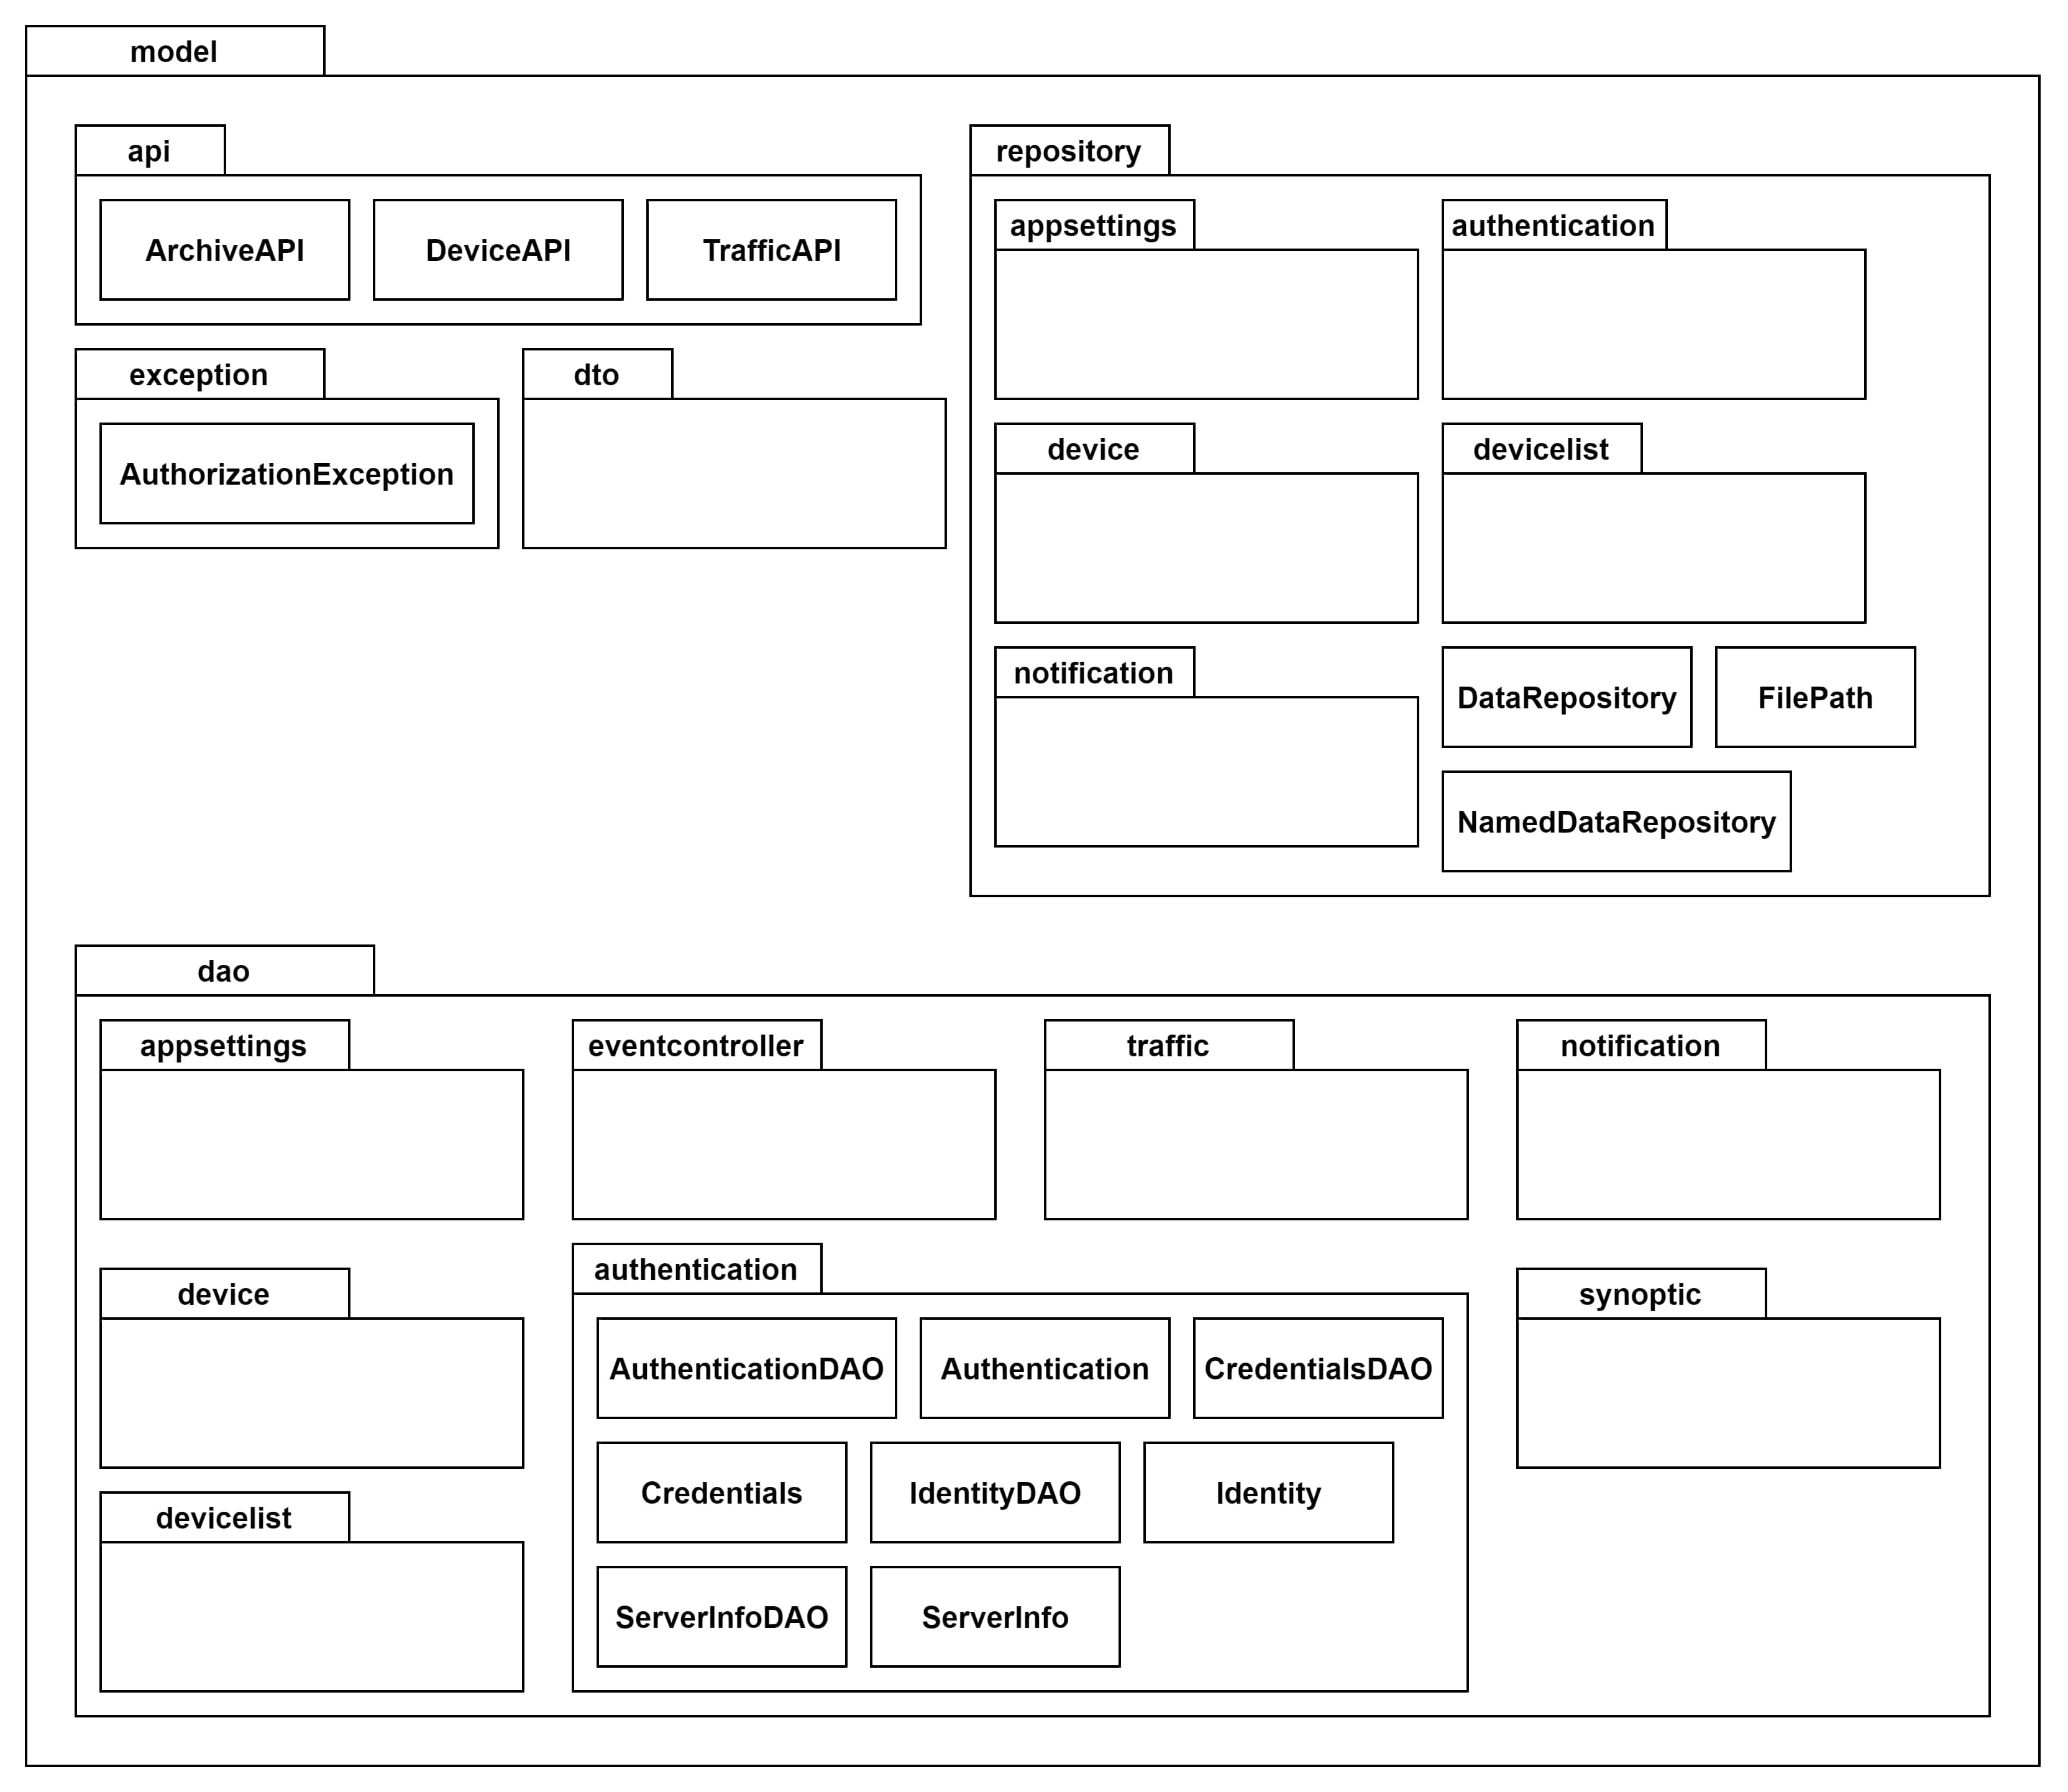
\includegraphics[width=1.0\columnwidth]{capitolo-6/organizzazione-package/model} 
  \caption{Diagramma del package \texttt{it.tecsen.smacs.model}}
\end{figure}
Questo package implementa il modello dell'applicazione.\\
Si può dividere in più aree con compiti specifici, rappresentate dai sotto-package:
\begin{itemize}
  \item \texttt{api} contiene classi che utilizzano il wrapper del package \texttt{webserviceclient} per interrogare le \gls{restg} e ritornare il risultato sotto forma di \gls{dto};
  \item \texttt{exception} contiene eccezioni che possono essere generate dalle classi presenti in questo package;
  \item \texttt{repository} contiene interfacce e classi per memorizzare su supporto persistente (le implementazioni usano dei file come supporto persistente) i dati ricevuti dai \gls{dao};
  \item \texttt{dao} contiene tutti le classi \gls{dao} che sono necessarie ai membri del package \texttt{viewmodel} per funzionare. Utilizza i package \texttt{api} e \texttt{repository} per ottenere i dati da ritornare sotto forma di \gls{dto};
  \item \texttt{dto} contiene tutti le classi \gls{dto} che sono necessarie al funzionamento dei package \texttt{api}, \texttt{dao} e \texttt{viewmodel}.
\end{itemize}
Sebbene \texttt{api} e \texttt{dao} ritornino entrambi \gls{dto}, c'è una differenza:
\begin{itemize}
  \item il primo non fa nessuna elaborazione sui dati, semplicemente li ottiene dalle \gls{restg} sotto forma di \gls{json}, ne fa il parsing e restituisce quanto ottenuto;
  \item il secondo elabora i \gls{dto} ottenuti dal primo e li ritorna elaborati (per fare un esempio, una lista ricevuta da \texttt{api} potrebbe essere ordinata, filtrata e poi ritornata).
\end{itemize}

%**************************************************************
\subsubsection{Package it.tecsen.smacs.webserviceclient}
\label{subsubsubsec:it-tecsen-smacs-webserviceclient}

\begin{figure}[!h]
  \centering 
  
\includegraphics[width=1.0\columnwidth]{capitolo-6/organizzazione-package/webserviceclient} 
  \caption{Diagramma del package \texttt{it.tecsen.smacs.webserviceclient}}
\end{figure}
In questo package vi sono tutte le classi che implementano il wrapper della libreria \emph{http}, come è stato precedentemente illustrato in "\hyperref[subsubsec:it-tecsen-smacs]{Package it.tecsen.smacs}".


%**************************************************************
\subsubsection{Package it.tecsen.smacs.widget}
\label{subsubsubsec:it-tecsen-smacs-widget}

Il package \texttt{widget} non è stato riportato sotto forma diagrammatica per due ragioni:
\begin{itemize}
  \item perché è troppo vasto e dispersivo;
  \item perché contiene solo classi il cui scopo è permettere quanto più riuso di codice possibile per la parte di interfaccia utente.
\end{itemize}

%**************************************************************
\subsubsection{Package it.tecsen.smacs.config}
\label{subsubsubsec:it-tecsen-smacs-config}

Il package \texttt{config} non è stato riportato sotto forma diagrammatica perché come indicato in in "\hyperref[subsubsec:it-tecsen-smacs]{Package it.tecsen.smacs}" contiene principalmente configurazioni per il funzionamento di altre classi.

%**************************************************************
\subsection{Il design pattern Observer: Provider, ChangeNotifier e Consumer}
\label{subsec:observer-provider-changenotifier}

È stato detto che una delle caratteristiche dell'architettura MVVM è la presenza di un doppio Observer.\\
L'Observer è un \gls{designpatterng} formalizzato dalla "Gang of Four" nel libro \emph{Design Patterns - Elementi per il riuso di software ad oggetti}.\\
Permette:
\begin{itemize}
  \item di avere dipendenze di tipo "1 a molti" fra oggetti, permettendo di avere consistenza in maniera agevole;
  \item divide gli oggetti possessori di stato nella categoria \emph{Subject} e quelli che dipendono da questo stato in \emph{Observer};
  \item quando un \emph{Subject} aggiorna il suo stato notifica i propri \emph{Observer} (internamente dispone di un riferimento per ciascuno di questi, ma non sa nulla di loro per via dell'astrazione).
\end{itemize}
Di seguito viene presentato un esempio per illustrare come è stato implementato il \gls{designpatterng} Observer all'interno del prodotto.
L'esempio si riferisce alla parte del sistema in cui un \emph{ViewModel} ha ricevuto dai \gls{dao} da cui dipende una nuova lista e quindi notifica qualsiasi \emph{View} in ascolto.
Solo alcune parti (quelle fondamentali ai fini dell'esempio) vengono riportate.

%**************************************************************
\subsubsection{Il Subject: ChangeNotifier}
\label{subsubsec:subject-changenotifier}

In \emph{Flutter} (e non Dart, perché è propriamente una caratteristica del \gls{frameworkg}) un \emph{Subject} è realizzabile molto semplicemente aggiungendo nella firma di una classe il mixin \texttt{ChangeNotifier}, come mostrato di seguito:

\begin{lstlisting}
class DeviceList with ChangeNotifier implements DeviceListVM {
  ...

  DeviceListDAO _deviceListDAO;
  
  ...
}
\end{lstlisting}
In questa porzione di classe sono messi in vista anche \texttt{DeviceListVM}, che è la dipendenza di cui necessita la \emph{View} e \texttt{DeviceListDAO} che è invece una dipendenza di questo \emph{ViewModel}.\\
Nel metodo in cui viene aggiornato lo stato avviene anche la notifica degli \emph{Observer}:
\begin{lstlisting}
@override
Future<void> syncDeviceList({final bool forceDownload = false}) async {
    ...

    await _deviceListDAO.syncDeviceList(_token, _deviceTree, forceDownload: forceDownload);

    notifyListeners();
}
\end{lstlisting}
Come si può notare, dopo aver chiamato il metodo \texttt{syncDeviceList} di \texttt{DeviceListDAO} a riga 5, viene invocato il metodo \texttt{notifyListeners} che appartiene al \emph{mixin} \texttt{ChangeNotifier}.\\
Una volta ricevuta la notifica, uno dei primi metodi che viene richiamato dalla vista è quello che ritorna la cardinalità della lista che è appena stata scaricata (successivamente seguono altre chiamate), in base alla selezione dell'utente:
\begin{lstlisting}
@override
Future<int> get selectedDeviceListLength async {
  List<Device> devices;

  if (_activeDisplayMode == DisplayMode.ALPHABETICAL_ORDER) {
    devices = _deviceListDAO.alphabeticalOrderDeviceList;
  } else {
    devices = _deviceListDAO.warningDeviceList;
  }

  if (_nearbyDevicesMode) {
    devices = await _deviceListDAO.nearbyDeviceList(deviceList);
  }

  return devices.length;
}
\end{lstlisting}
I due costrutti \texttt{if} servono a verificare che tipo di lista va ritornata all'utente (in base alle sue precedenti selezioni), per invocare il metodo corretto.

%**************************************************************
\subsubsection{Il Subject: Provider}
\label{subsubsec:subject-provider}

Come è stato già illustrato al capitolo 5 sulla "\hyperref[cap:dependency-injection]{Dependency Injection}", un'istanza di \texttt{DeviceListVM} va messa a disposizione dei widget figli attraverso un \emph{Provider} come antenato nel \emph{Widget tree}.\\
In questo caso, visto che \texttt{DeviceListVM} usa \texttt{ChangeNotifier} ed ha delle dipendenze esterne (due, per l'esattezza), viene istanziato un \texttt{ChangeNotifierProxyProvider2}.
\begin{lstlisting}
class DeviceListScreen extends StatelessWidget {
  ...

  @override
  Widget build(BuildContext context) {
    return ChangeNotifierProxyProvider2<IdentityDAO, DeviceListDAO, DeviceListVM>(
      // Viene creata l'istanza ma non viene usata 
      // (non ha i riferimenti ai DAO).
      create: (_) => DeviceList(),
      // Viene aggiornata l'istanza con i nuovi DAO.
      update: (_, identityDao, deviceListDao, deviceListVM) {
        deviceListVM.deviceListDAO = deviceListDao;
        deviceListVM.identityDAO = identityDao;
        return deviceListVM;
      },

      ...
    );
  }
}
\end{lstlisting}
In \texttt{ChangeNotifierProxyProvider2} il parametro \texttt{update} gestisce il caso in cui le dipendenze di \texttt{DeviceListVM} chiamino anche loro \texttt{notifyListeners}.

%**************************************************************
\subsubsection{L'Observer: Consumer}
\label{subsubsec:observer-consumer}

Un altro modo per chiamare il \gls{designpatterng} Observer è "Producer-Consumer", in cui il \emph{Producer} corrisponde al \emph{Subject} e l'\emph{Observer} corrisponde al \emph{Consumer}.\\
Senza troppa fantasia, un widget che in \emph{Flutter} si occupa di agire da \emph{Consumer} ha proprio questo nome: si registra come \emph{Observer} rispetto ad un \emph{ChangeNotifier} e ogni volta che riceve una notifica ricostruisce il suo sotto albero (la porzione di \emph{Widget tree} radicata nel suo primo discendente).
% Extra a capo per arrivare a fine pagina
\clearpage

\begin{lstlisting}
class DeviceListScreen extends StatelessWidget {
  ...

  @override
  Widget build(BuildContext context) {
    ...
  
    return ChangeNotifierProxyProvider2<IdentityDAO, DeviceListDAO, DeviceListVM>(
      child: Consumer<DeviceListVM>(
        // Il terzo parametro, noRedraw, corrisponde ad un widget che non va ricostruito nel caso DeviceListVM emetta notifiche.
        builder: (_, deviceListVM, noRedraw) {
          return ScreenViewSafeContainer(
            child: DeviceListView(),
            bottomAppBar: FutureBuilder<int>(
            future: deviceListVM.selectedDeviceListLength,
            ...
          );
        }
        ...
      ),
    );
  }
}
\end{lstlisting}
Come si può notare si è continuato l'esempio di prima (è la stessa classe e lo stesso metodo \texttt{build}).\\
Come affermato poc'anzi, ad ogni \texttt{notifyListeners} invocato da \texttt{DeviceListVM}, verrà ricostruito il sottoalbero radicato nel primo discendente disponibile del widget \texttt{Consumer}, ovvero \texttt{ScreenViewSafeContainer} (propriamente viene invocato nuovamente il \emph{callback} \texttt{builder} a riga 11, ma è un dettaglio del \gls{frameworkg} che non cambia il principio di funzionamento).

%**************************************************************
\section{Confronto fra la precedente app e quella nuova}
\label{sec:confronto-precedente-app-nuova}

In questa sezione vengono mostrate le differenze più significative fra la precedente app (in uso presso l'azienda) e quella nuova, realizzata durante lo stage.\\
Queste differenze sono dovute principalmente alla richiesta da parte del tutor aziendale di pensare a come poter fare un restyling grafico dell'applicazione che attualmente hanno in uso.
Quest'ultima infatti, essendo un po' datata, è stata progettata con un impianto grafico e con un'esperienza utente diverse da quelle da quelle attuali.\\
Innanzitutto, gli schermi degli smartphone e dei tablet sono, negli ultimi anni, diventati sempre più grandi e con risoluzioni più elevate, offrendo più spazio per disporre il contenuto di una schermata.
Non ha quindi più senso, ad esempio, avere liste scorrevoli di elementi che sono condensate. Ci si può permettere di spaziare molto di più gli elementi e anche migliorare anche lo spazio fra una linea di testo e un'altra.\\
Inoltre, entrambi i sistemi operativi per cui sviluppare l'applicazione hanno un loro stile grafico, per cui va valutato se creare due interfacce utenti del tutto simili ma con componenti che ricalcano quelle native oppure cercare di creare un'interfaccia che possa andare bene per entrambe, evitando di utilizzare componenti grafiche specifiche per l'uno o per l'altro sistema.
Ad esempio, nel \emph{Material Design} di Google vi sono delle componenti chiamate \emph{Floating Action Button} (dei pulsanti a forma circolare posizionati solitamente in basso al centro/destra che "fluttuano" sopra il contenuto), da utilizzare come pulsanti per svolgere azioni come la modifica di contenuti testuali, che in Android si integrerebbero correttamente, in iOS invece no.\\
Un'altra riflessione che è stata fatta è relativa ai menu principale dell'applicazione: come viene mostrato in "\hyperref[subsec:menu-applicazione]{Menu dell'applicazione}", difficilmente viene ancora usato un menu a tendina per mostrare funzionalità secondarie, preferendo invece un menu di tipo "drawer".\\
Altre considerazioni e dimostrazione dei miglioramenti apportati si possono trovare nelle sotto-sezioni che seguono.

% \clearpage % Tenere se non viene scritto altro in questa sezione.

%**************************************************************
\subsection{Informazioni sull'applicazione}
\label{subsec:informazioni-applicazione}

Questa schermata è disponibile aprendo il menu dell'applicazione (schermata che viene presentata in seguito a questa) e mostra informazioni generali sull'applicazione, tra cui il server a cui si è connessi, il nome utente e la versione.\\
Il contenuto di questa schermata, che nella app dell'azienda è condensato verso l'alto, viene ora reso più spaziato e inserito in più elementi di una lista scorrevole permettendo, in futuro, di aggiungere contenuti alla schermata senza problemi.\\
I due loghi, dell'azienda presso cui si è svolto lo stage e dell'azienda di cui è partner, sono stati resi cliccabili ed entrambi reindirizzano al rispettivo sito web.

\begin{figure}[!h]
  \centering 
  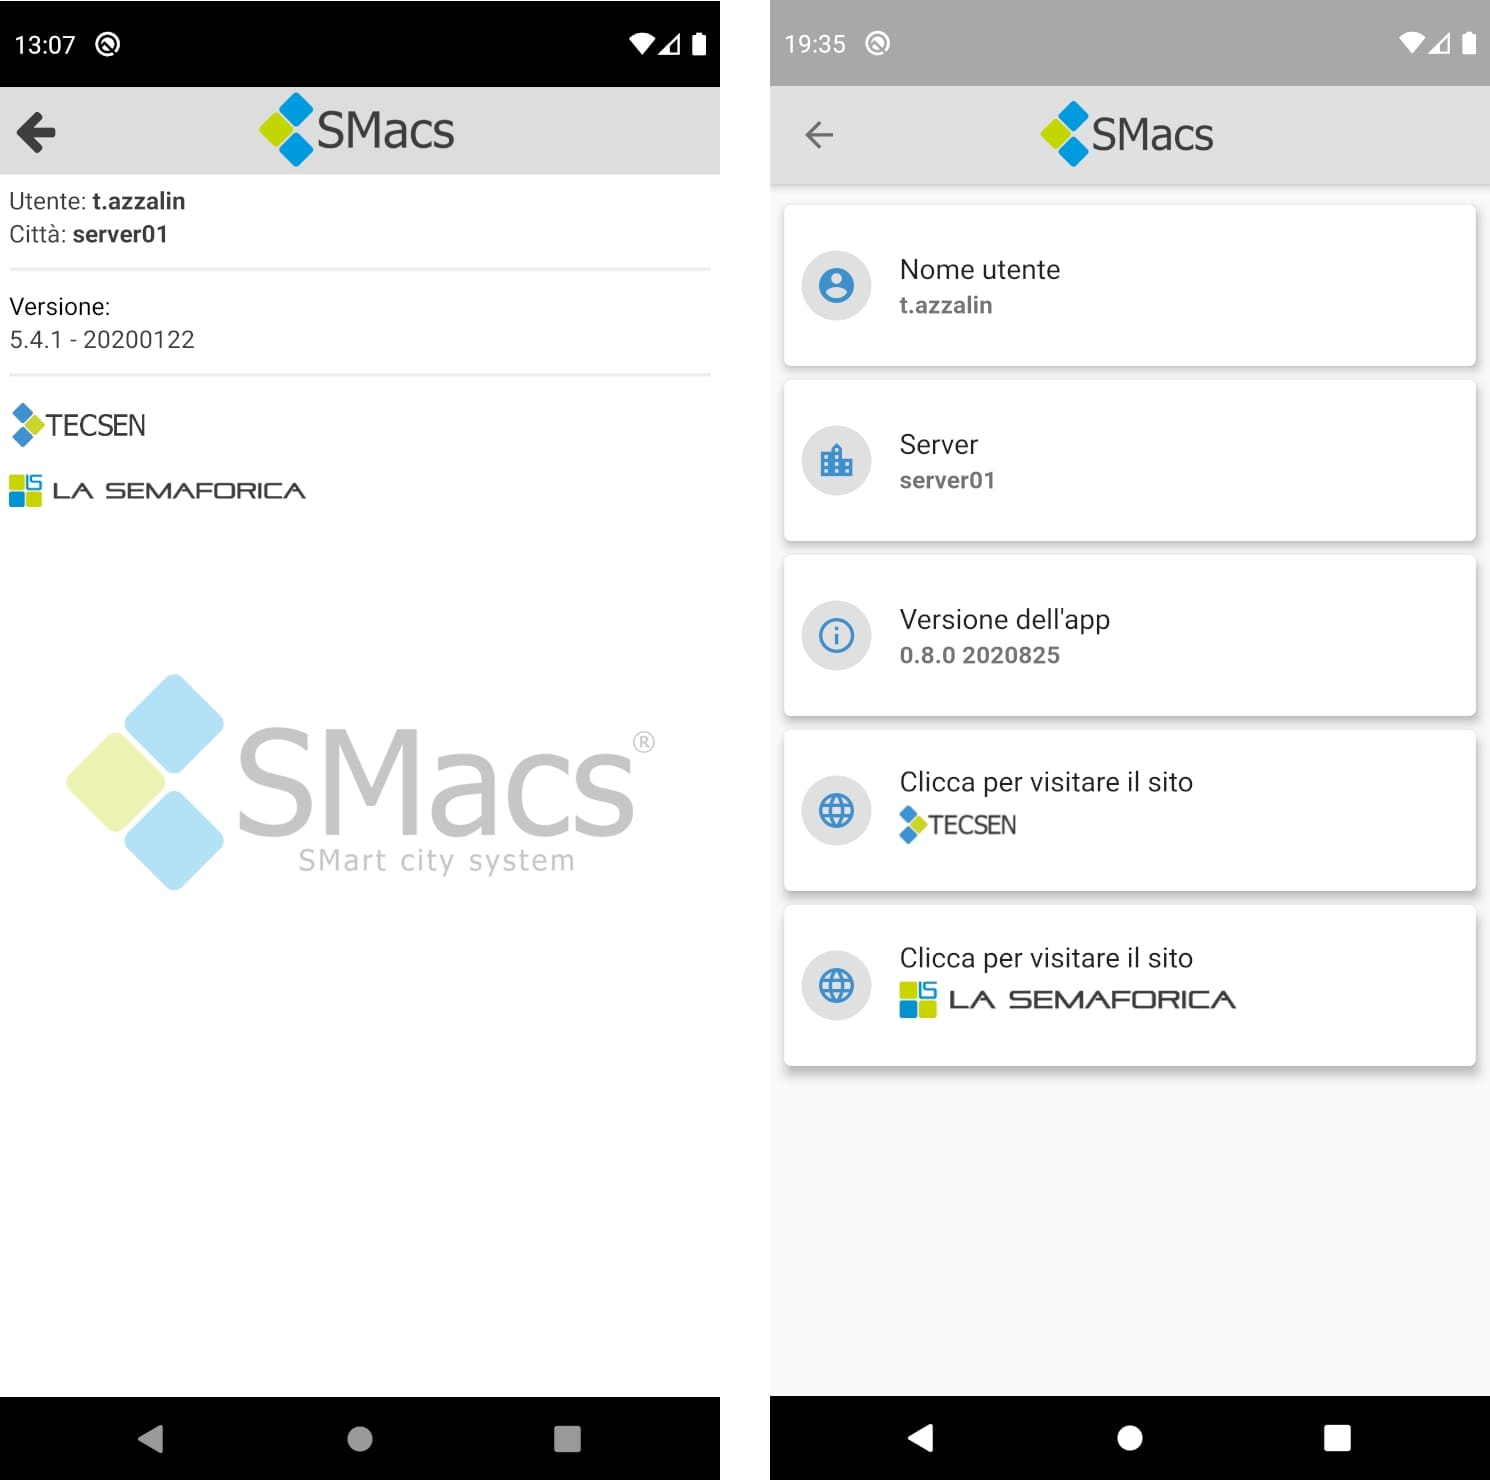
\includegraphics[width=0.75\columnwidth]{capitolo-6/confronto-app-vecchia-nuova/AppInfoView} 
  \caption{Confronto fra schermate delle app: Informazioni sull'applicazione}
\end{figure}

\clearpage % Tenere per assicurarsi che ci sia un'immagine per pagina e basta.

%**************************************************************
\subsection{Menu dell'applicazione}
\label{subsec:menu-applicazione}

Il menu dell'applicazione è accessibile, così come nell'app dell'azienda, solamente attraverso la schermata della lista degli impianti.\\
Prima disponibile sotto forma di menu a tendina, nella versione realizzata per lo stage è stato realizzato un menu di tipo \emph{drawer} (dall'inglese, cassetto, perché alla richiesta di apertura effettua una transizione dall'esterno all'interno e si richiude in maniera inversa), che appare da sinistra alla pressione del pulsante \emph{hamburger} (il pulsante con tre linee parallele orizzontali è stato così ribattezzato perché assomiglia ad un panino di un fast food) in alto a sinistra (visibile nella schermata di destra nell'immagine sottostante).\\
Le voci del menu sono state mantenute così com'erano ad eccezione della voce "Refresh", che aggiorna la lista di impianti disponibile localmente riscaricandola dai server aziendali, che è stata rimossa in favore di un più accessibile pulsante presente direttamente nella barra di navigazione in alto alla schermata, riducendo il numero di click necessari per raggiungerlo.

\begin{figure}[!h]
  \centering 
  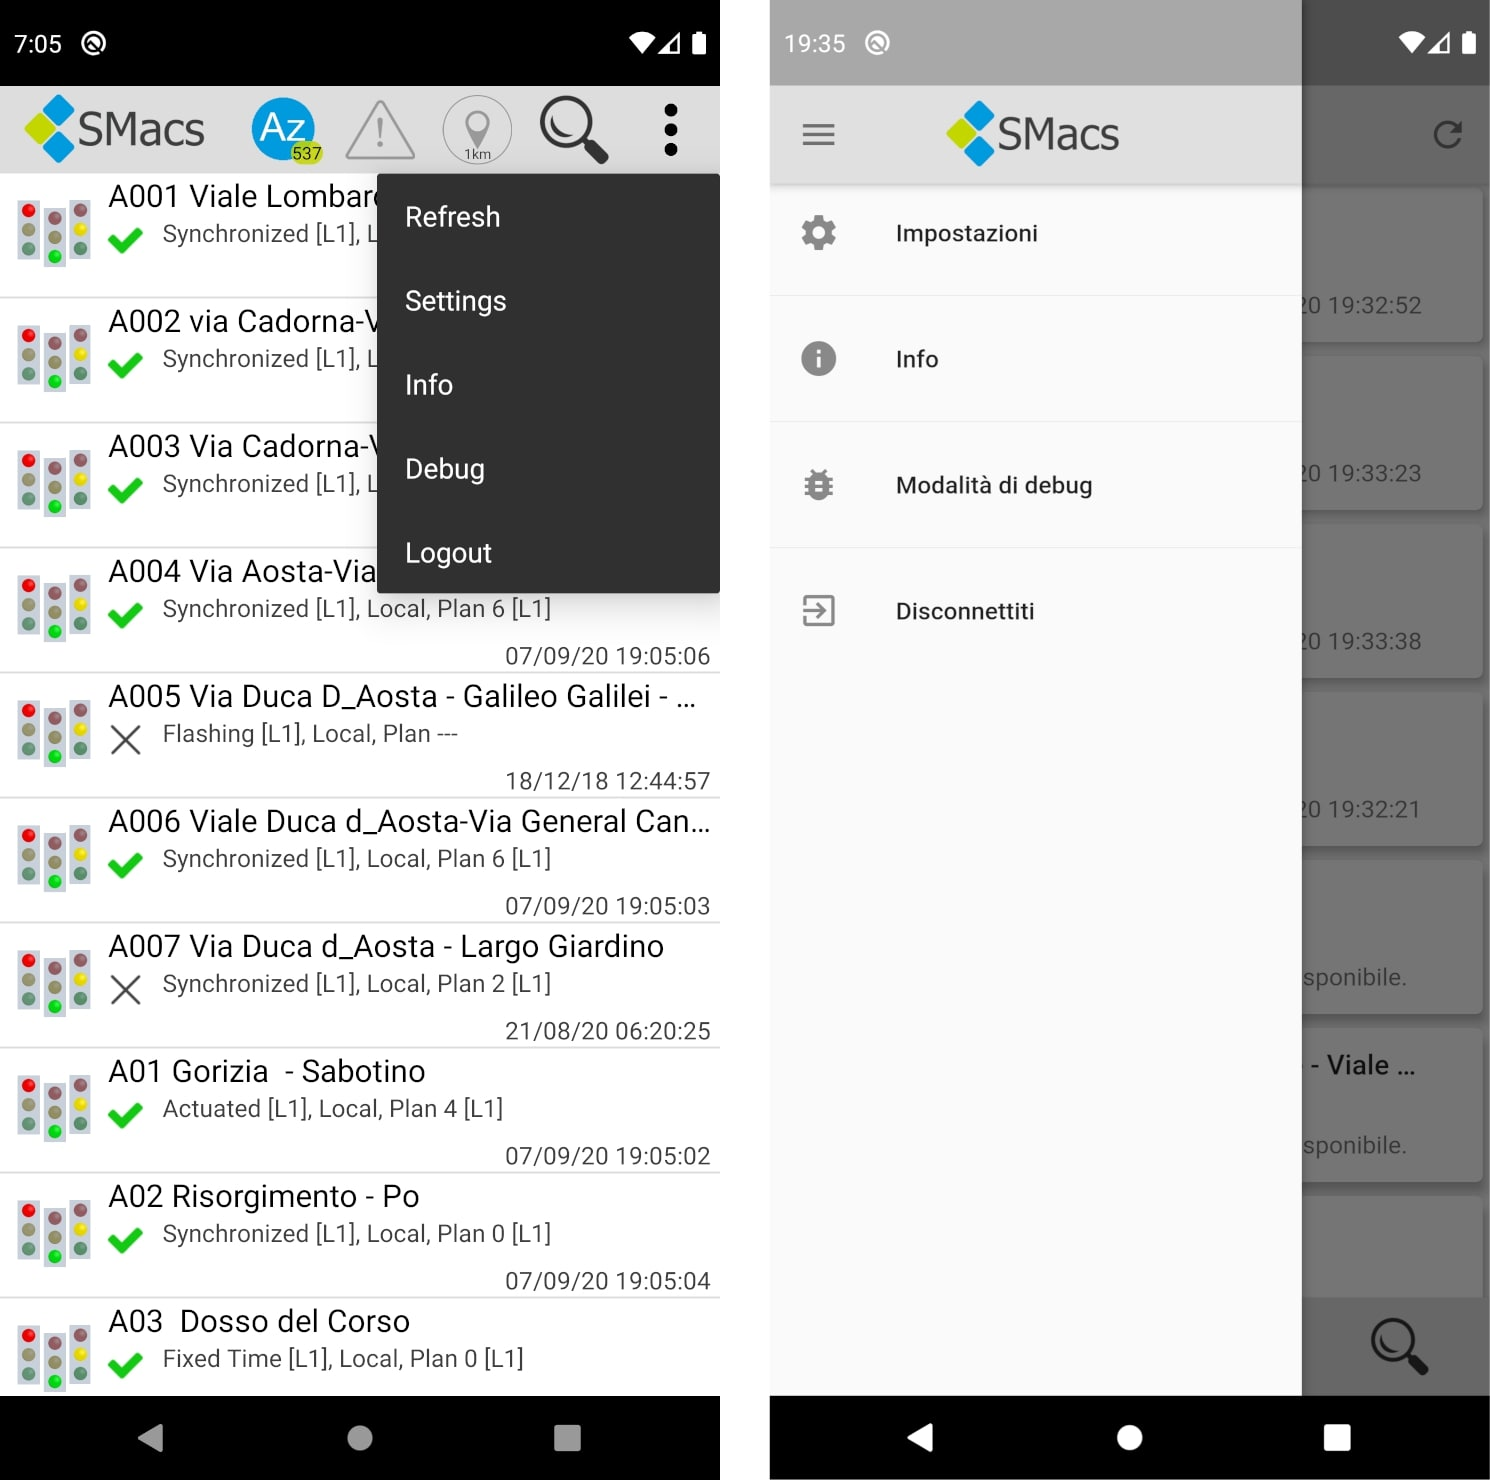
\includegraphics[width=1.0\columnwidth]{capitolo-6/confronto-app-vecchia-nuova/DrawerView} 
  \caption{Confronto fra schermate delle app: Menu dell'applicazione}
\end{figure}

\clearpage % Tenere per assicurarsi che ci sia un'immagine per pagina e basta.

%**************************************************************
\subsection{Lista degli impianti}
\label{subsec:lista-impianti}

La schermata in cui viene mostrata la lista degli impianti è rimasta sostanzialmente invariata se non per alcune modifiche prettamente estetiche.\\
I pulsanti per filtrare la lista sono stati spostati dalla barra di navigazione in alto a una barra apposita in basso e, come è stato detto in precedenza, il pulsante di "Refresh" è stato estratto dal menu per averlo disponibile nella barra di navigazione.\\
A differenza dell'applicazione in uso presso l'azienda, non tutte le funzionalità sono disponibili: tutti gli elementi della lista la cui icone rappresentano dei semafori sono cliccabili (e portano alla schermata di dettaglio) mentre gli altri, come i primi due elementi della lista della schermata di destra, non lo sono.\\
In quest'ultimo caso, la pressione dell'elemento visualizza un avviso all'utente che lo informa sul fatto che la funzionalità non è ancora disponibile.

\begin{figure}[!h]
  \centering 
  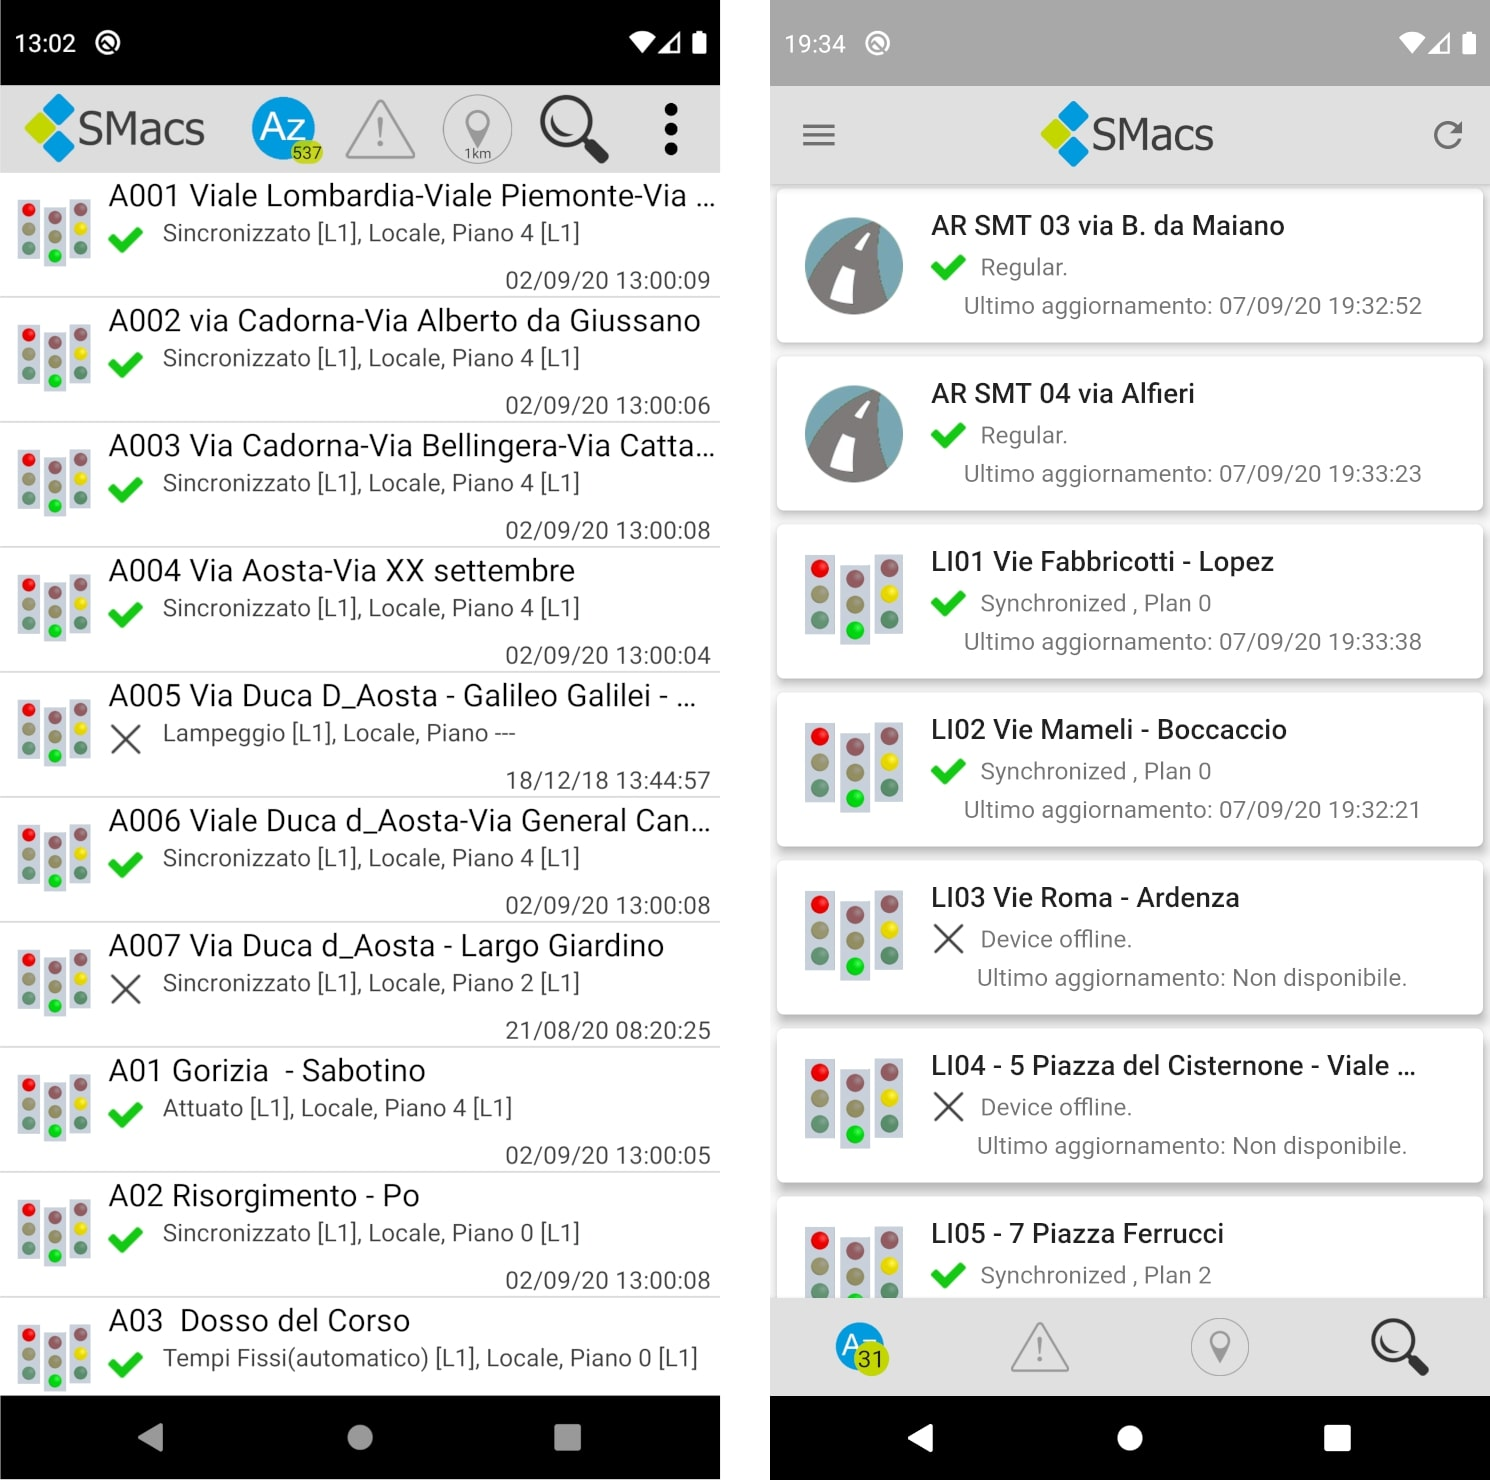
\includegraphics[width=1.0\columnwidth]{capitolo-6/confronto-app-vecchia-nuova/DeviceListView} 
  \caption{Confronto fra schermate delle app: Lista degli impianti}
\end{figure}

\clearpage % Tenere per assicurarsi che ci sia un'immagine per pagina e basta.

%**************************************************************
\subsection{Pannello di controllo}
\label{subsec:pannello-controllo}

La schermata del dettaglio di un regolatore semaforico è cambiata sensibilmente.\\
Questa schermata comprende tutta ciò che è presente nell'immagine di destra, incluse le tre schede "Panoramica", "Diagnostica", "Pannello di controllo" e il loro contenuto.
Dalla pulsantiera in basso sono stati rimossi il "Pannello di controllo", che è appunto diventata una scheda, e il pulsante "Indicazioni stradali", giustificato dal fatto che premendo il pulsante "Posizione" si apre l'applicazione di mappe del dispositivo, che già propone l'avvio nella navigazione.\\
È stato invece inserito il pulsante "Info" che rimanda alla schermata con le informazioni dell'hardware e del software del regolatore semaforico.\\
Oltre a queste modifiche, che sono comuni a "Panoramica" e a "Diagnostica", nella schermata "Pannello di controllo" è stata semplificata l'interfaccia, rendendola più simile a quella attualmente usata negli applicativi per desktop dell'azienda (a fini di unificazione dell'esperienza utente).
In particolare, la pulsantiera "Funzione" è diventata un menu a tendina, "Reset allarmi" è stata spostata nella scheda "Diagnostica" e le altre funzionalità è stato chiesto di non inserirle.

\begin{figure}[!h]
  \centering 
  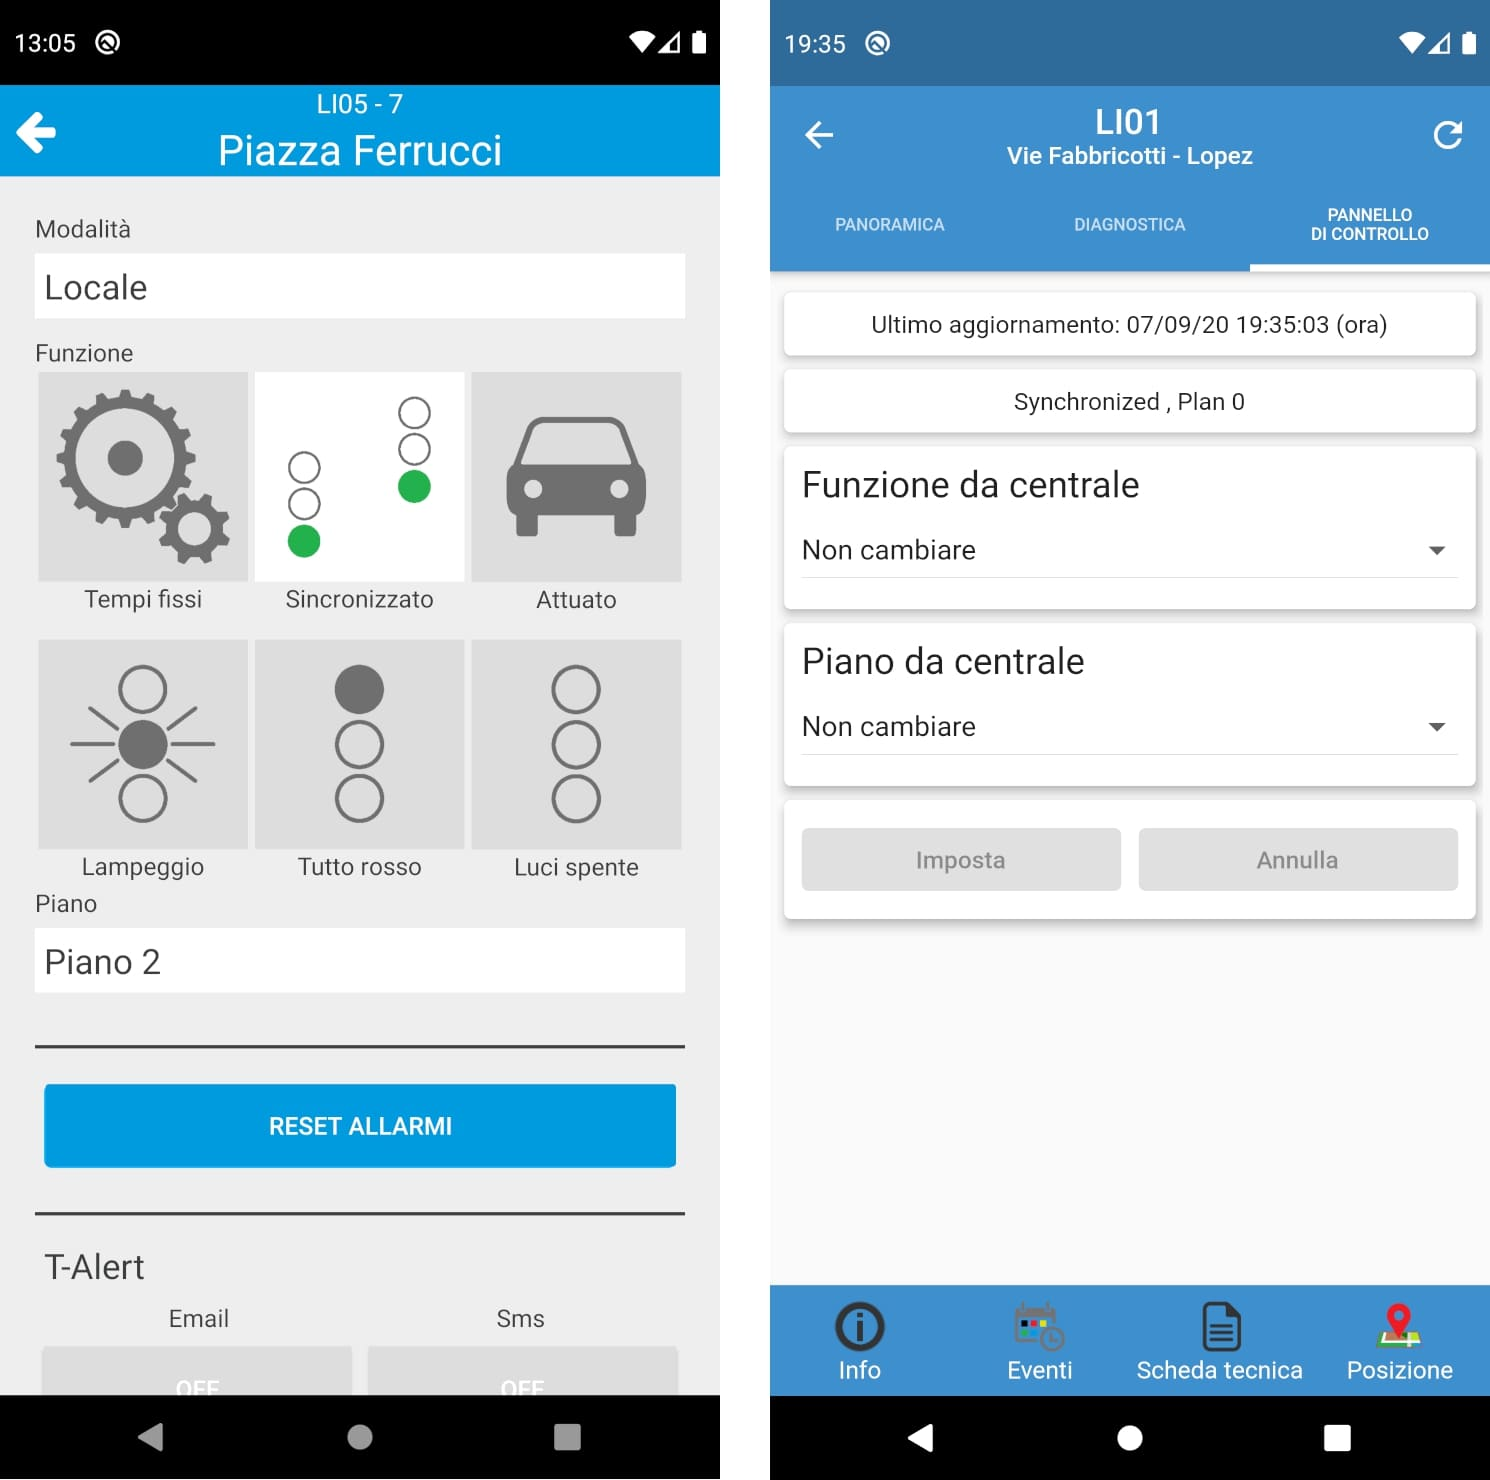
\includegraphics[width=1.0\columnwidth]{capitolo-6/confronto-app-vecchia-nuova/ControlPanelView} 
  \caption{Confronto fra schermate delle app: Pannello di controllo}
\end{figure}

\clearpage % Tenere per assicurarsi che ci sia un'immagine per pagina e basta.

%**************************************************************
\subsection{Panoramica sull'impianto}
\label{subsec:panoramica-impianto}

Come precedentemente affermato, la schermata del dettaglio è cambiata sensibilmente.\\
Dopo aver elencato i cambiamenti avvenuti nella scheda "Pannello di controllo" e nella pulsantiera in basso alla schermata, possiamo notare come tutte le icone di semafori e degli input (le icone sottostanti) siano state rimosse e le informazioni testuali semplificate.\\
Le icone appena citate sono state rimosse perché rappresentano le stesse che sono posizionate sopra l'immagine dell'intersezione stradale nella schermata di destra.
Questa funzionalità di visione dell'intersezione è chiamata \emph{sinottico} ed è disponibile attualmente nell'app aziendale previa pressione del pulsante a forma di intersezione stradale, situato accanto all'icona di aggiornamento, in alto a destra della schermata di sinistra.\\
Infine, la lista dei messaggi di diagnostica (nell'immagine di sinistra, quella che parte dal centro, sotto la scritta "Dettagli - 1 Info") è stata spostata nella scheda "Diagnostica".

\begin{figure}[!h]
  \centering 
  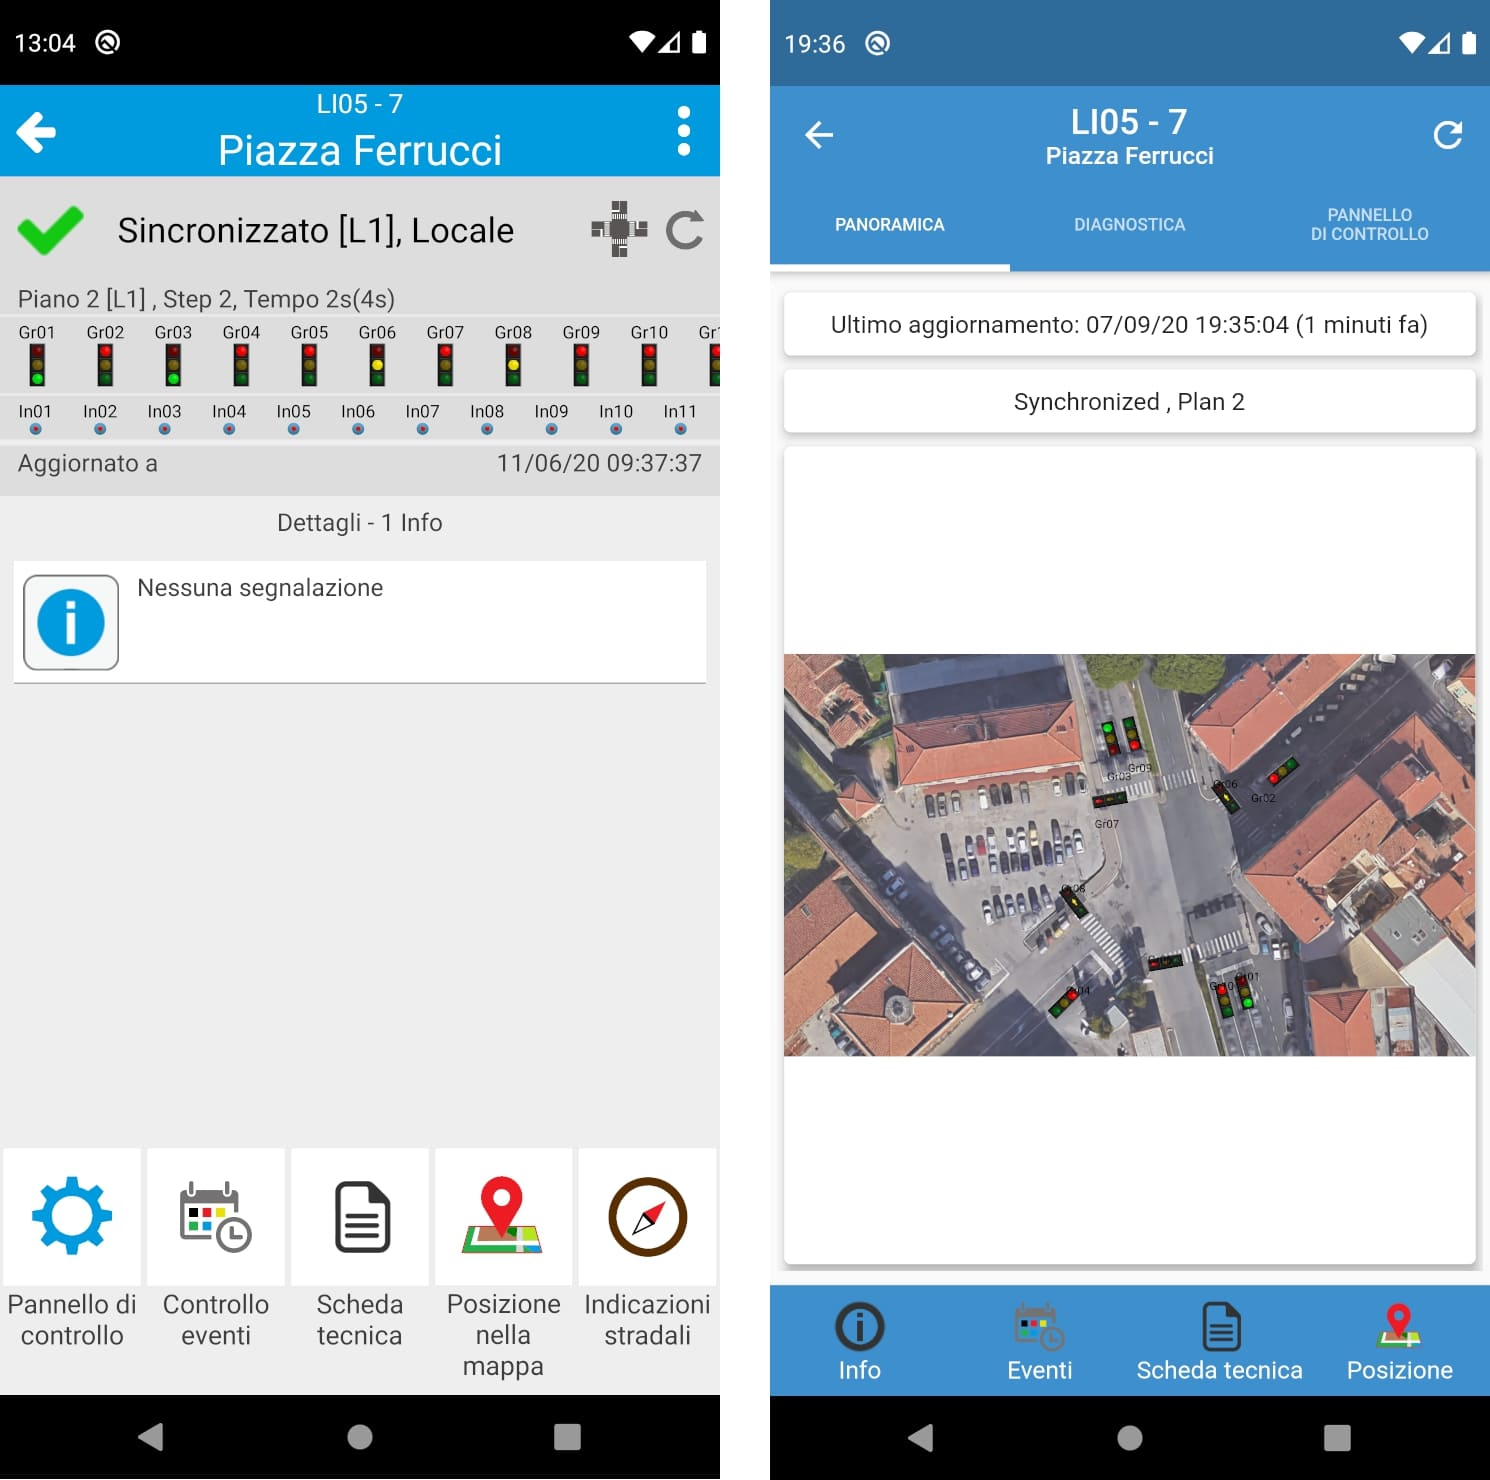
\includegraphics[width=1.0\columnwidth]{capitolo-6/confronto-app-vecchia-nuova/DeviceOverviewView} 
  \caption{Confronto fra schermate delle app: Panoramica sull'impianto}
\end{figure}             % Prodotto dello stage
% !TEX encoding = UTF-8
% !TEX TS-program = pdflatex
% !TEX root = ../tesi.tex

%**************************************************************
\chapter{Conclusioni}
\label{cap:conclusioni}
%**************************************************************

\intro{
   In questo capitolo si vogliono trarre delle conclusioni sull'esperienza svolta e sulla sua importanza, tornando nuovamente sulle conoscenze acquisite e sugli obiettivi raggiunti. Infine, vengono presentati alcuni spunti per migliorare il prodotto software realizzato durante lo stage.
}\\

%**************************************************************
\section{Obiettivi raggiunti}
\label{sec:obiettivi-raggiunti}

Vengono riproposti di seguito gli obiettivi che erano stati concordati nel Piano di Lavoro. Assieme a questi, vengono aggiunti il restyling grafico (introdotto in "\hyperref[sec:requisiti-obiettivi-finali]{Requisiti e obiettivi finali}") e un obiettivo riepilogativo che include tutti i casi d'uso presenti nell'appendice "\hyperref[cap:analisi-dei-requisiti]{Analisi dei requisiti}".

{
\renewcommand{\arraystretch}{1.5}
\begin{longtable}{|C{9cm}|c|}
    \hline
    \textbf{Obiettivo} & \textbf{Completamento} \\\hline
    \endhead
    Realizzazione dell'applicazione con una tecnologia multipiattaforma. & Completato\\\hline
    Reperimento dei dati per l'applicazione attraverso \gls{restg}. & Completato \\\hline
    Realizzazione di un task in background nell'applicazione per la verifica della presenza di nuovi dati per l'utente. & Completato \\\hline
    Internazionalizzazione dell'applicazione (in lingue italiana e inglese, ma estendibile ad altre). & Completato \\\hline
    Comprensione su come generare i pacchetti dell'applicazione da rilasciare ai clienti. & Completato \\\hline
    Restyling grafico dell'interfaccia utente dell'attuale applicazione per lo sviluppo della nuova. & Completato \\\hline
    Implementazione dei casi d'uso analizzati. & Completato \\\hline
    \caption{Raggiungimento degli obiettivi}
\end{longtable}
}

%**************************************************************
\section{Conoscenze acquisite}
\label{sec:conoscenze-acquisite}

Questa esperienza di stage è stata molto istruttiva sia da un punto di vista umano che informatico, strettamente legato al lavoro.\\
Dal punto di vista umano, è stato utile per comprendere come avvengono le relazioni all'interno di un'azienda e come vengono condivise le opinioni e le idee su un obiettivo comune da raggiungere.\\
Dall'altro, ha permesso di consolidare quanto appreso durante questi tre anni di studi, permettendo di apprendere inoltre:
\begin{itemize}
    \item le tecnologie disponibili ad uno sviluppatore che deve realizzare un'applicazione multipiattaforma;
    \item come realizzare applicazioni con \emph{Flutter} e Dart;
    \item come utilizzare svariate librerie per \emph{Flutter} e Dart, tra cui \emph{Provider}, \emph{http}, \emph{workmanager} e \emph{flutter\_local\_notifications};
    \item come strutturare un progetto software seguendo un design pattern architetturale (MVVM, in questo caso) e altri design pattern (come Observer);
    \item come gestire i permessi da richiedere all'utente per un applicazione Android e iOS.
\end{itemize}

%**************************************************************
\section{Considerazioni finali sull'esperienza di stage}
\label{sec:considerazioni-finali}

Uno stage a conclusione di un ciclo di studi ritengo sia immensamente importante.\\
Dopo aver visto, nel corso degli studi, diversi aspetti dell'informatica, più o meno pratici, appresi più linguaggi e tecnologie e "concluso" con il progetto del corso di Ingegneria del software, permette di chiudere un cerchio.
Offre allo studente di applicare quanto imparato fino a quel momento e di concretizzarlo in un progetto elaborato assieme ad un'azienda, coniugando le esigenze educative, dello studente, e lavorative, dell'azienda.\\
In particolare, lo studente può rendersi conto di come si affrontano realmente i problemi in ambito lavorativo, quali sono le necessità e i rapporti fra persone all'interno di un'azienda.
In base a dove si svolge lo stage, può pur essere che si scoprano degli aspetti nella relazione fra l'azienda e i propri clienti e, sempre nel caso specifico dell'informatica, come le richieste di un cliente vengano prese in considerazione per poterle trasformare in un prodotto software che soddisfi le sue necessità.\\
Un altro aspetto fondamentale che si impara in parte già durante gli studi, ma in maniera ancora più concentrata durante lo stage, è la gestione dei tempi: avendo un tempo strettamente finito, bisogna saper coniugare gli obiettivi da raggiungere con le proprie disponibilità temporali.
Per fare un esempio, non è possibile sviluppare un prodotto con una tecnologia rispetto ad un'altra se farlo impiegherebbe più tempo di quanto disponibile, come non è altrettanto possibile non far caso a ritardi o a problemi che si incontrano durante il percorso.
Dal punto di vista lavorativo, si impara quindi a ragionare all'interno di certi vincoli, da un certo punto di vista necessari anche per il rispetto di sé stessi, e di sapervici rientrare ottenendo il miglior risultato possibile.

%**************************************************************
\section{Possibili sviluppi futuri per il prodotto}
\label{sec:sviluppi-futuri}

Il prodotto realizzato per lo stage consisteva nel realizzare solamente una porzione delle funzionalità attualmente presenti nell'applicazione su cui ci si basava. Quindi, le prime integrazioni da apportare sono di questa natura.\\
Altre possibili integrazioni possono essere:
\begin{itemize}
    \item aggiungere più lingue possibili a quelle disponibili, per rendere più pratico l'utilizzo dell'applicazione da parte di clienti di diverse nazionalità;
    \item sfruttare più efficientemente lo spazio a disposizione in modalità tablet, visualizzando la lista degli impianti sotto forma di griglia oppure visualizzando in una porzione della schermo la lista e nello spazio restante il dettaglio dell'impianto selezionato;
    \item rendere più accessibile l'applicazione, aggiungendo tooltip negli input, dove possibile;
    \item sfruttare le potenzialità del framework per adattare l'applicazione all'uso da browser;
    \item sostituire il sistema di monitoraggio intervallato in background con la ricezione di notifiche push inviate dal server (richiede però un aggiornamento del server).
\end{itemize}
             % Conclusioni
\appendix
% !TEX encoding = UTF-8
% !TEX TS-program = pdflatex
% !TEX root = ../tesi.tex

%**************************************************************
\chapter{Analisi dei requisiti}
\label{cap:analisi-dei-requisiti}
%**************************************************************

\intro{In questa appendice vengono illustrati i casi d'uso che sono stati implementati nell'applicazione realizzata durante lo stage. Si trovano in questa appendice poiché lo scopo del documento è presentare il processo decisionale che ha portato alla scelta di una tecnologia per realizzare un'applicazione e come si rapporta con altre tecnologie già conosciute, non parlare in dettaglio del prodotto realizzato. Questo capitolo è utile principalmente per comprendere lo scopo di alcune classi nella presentazione dei package, nel capitolo 6.}\\

%**************************************************************
\section{Introduzione}
\label{sec:introduzione-appendice}

I casi d'uso sono stati decisi la prima settimana di stage. Sono basati sull'applicazione in uso presso l'azienda ma hanno avuto alcuni adattamenti per rispecchiare meglio la nuova applicazione che si andava a realizzare.\\
I requisiti sono stati tratti completamente dai casi d'uso qui descritti.

%**************************************************************
\section{Attori}
\label{sec:attori}

Gli attori del sistema sono due e si distinguono per le operazioni che possono compiere:
\begin{itemize}
    \item \emph{Utente non autenticato}, che corrisponde all'utilizzatore del prodotto senza aver avuto accesso al sistema con le proprie credenziali;
    \item \emph{Utente autenticato}, che invece corrisponde all'utilizzatore del sistema dopo aver avuto accesso al sistema con successo con le proprie credenziali.
\end{itemize}

%**************************************************************
\section{Casi d'uso}
\label{sec:casi-uso}

I casi d'uso studiati per il prodotto sono stati realizzati sotto forma testuale, per una spiegazione dettagliata, e sotto forma di diagrammi.
Ciascuno testo descrittivo di un caso d'uso ne indica:
\begin{itemize}
    \item il \emph{codice identificativo}, nella forma $UCx.y.z$ con $x$, $y$ e $z$ numeri naturali;
    \item il \emph{nome}, che introduce brevemente il contesto applicativo del caso d'uso;
    \item gli \emph{attori principali} e \emph{attori secondari} (quest'ultimi se presenti), rispettivamente coloro che compiono l'azione indicata nel caso d'uso e coloro che invece aiutano a raggiungere le post-condizioni;
    \item lo \emph{scenario principale}, ovvero cosa può compiere l'utente con questo caso d'uso;
    \item le \emph{precondizioni}, ovvero lo stato del sistema antecedente l'esecuzione della funzionalità descritta;
    \item le \emph{postcondizioni}, ovvero lo stato del sistema alla fine dell'esecuzione della funzionalità descritta;
    \item le \emph{estensioni} (se presenti), ovvero una lista di casi d'uso che possono verificarsi sotto determinate condizioni che non permettono di raggiungere le postcondizioni indicate dal caso d'uso d'origine;
    \item le \emph{generalizzazioni} (se presenti), ovvero una lista di casi d'uso di cui il caso d'uso è implementazione più dettagliata.
\end{itemize}
I diagrammi dei casi d'uso (in inglese \emph{Use Case Diagram}) sono diagrammi realizzati in \gls{uml} dedicati alla descrizione delle funzioni o servizi offerti da un sistema, così come sono percepiti e utilizzati dagli attori che interagiscono col sistema stesso.

\begin{figure}[!h] 
    \centering 
    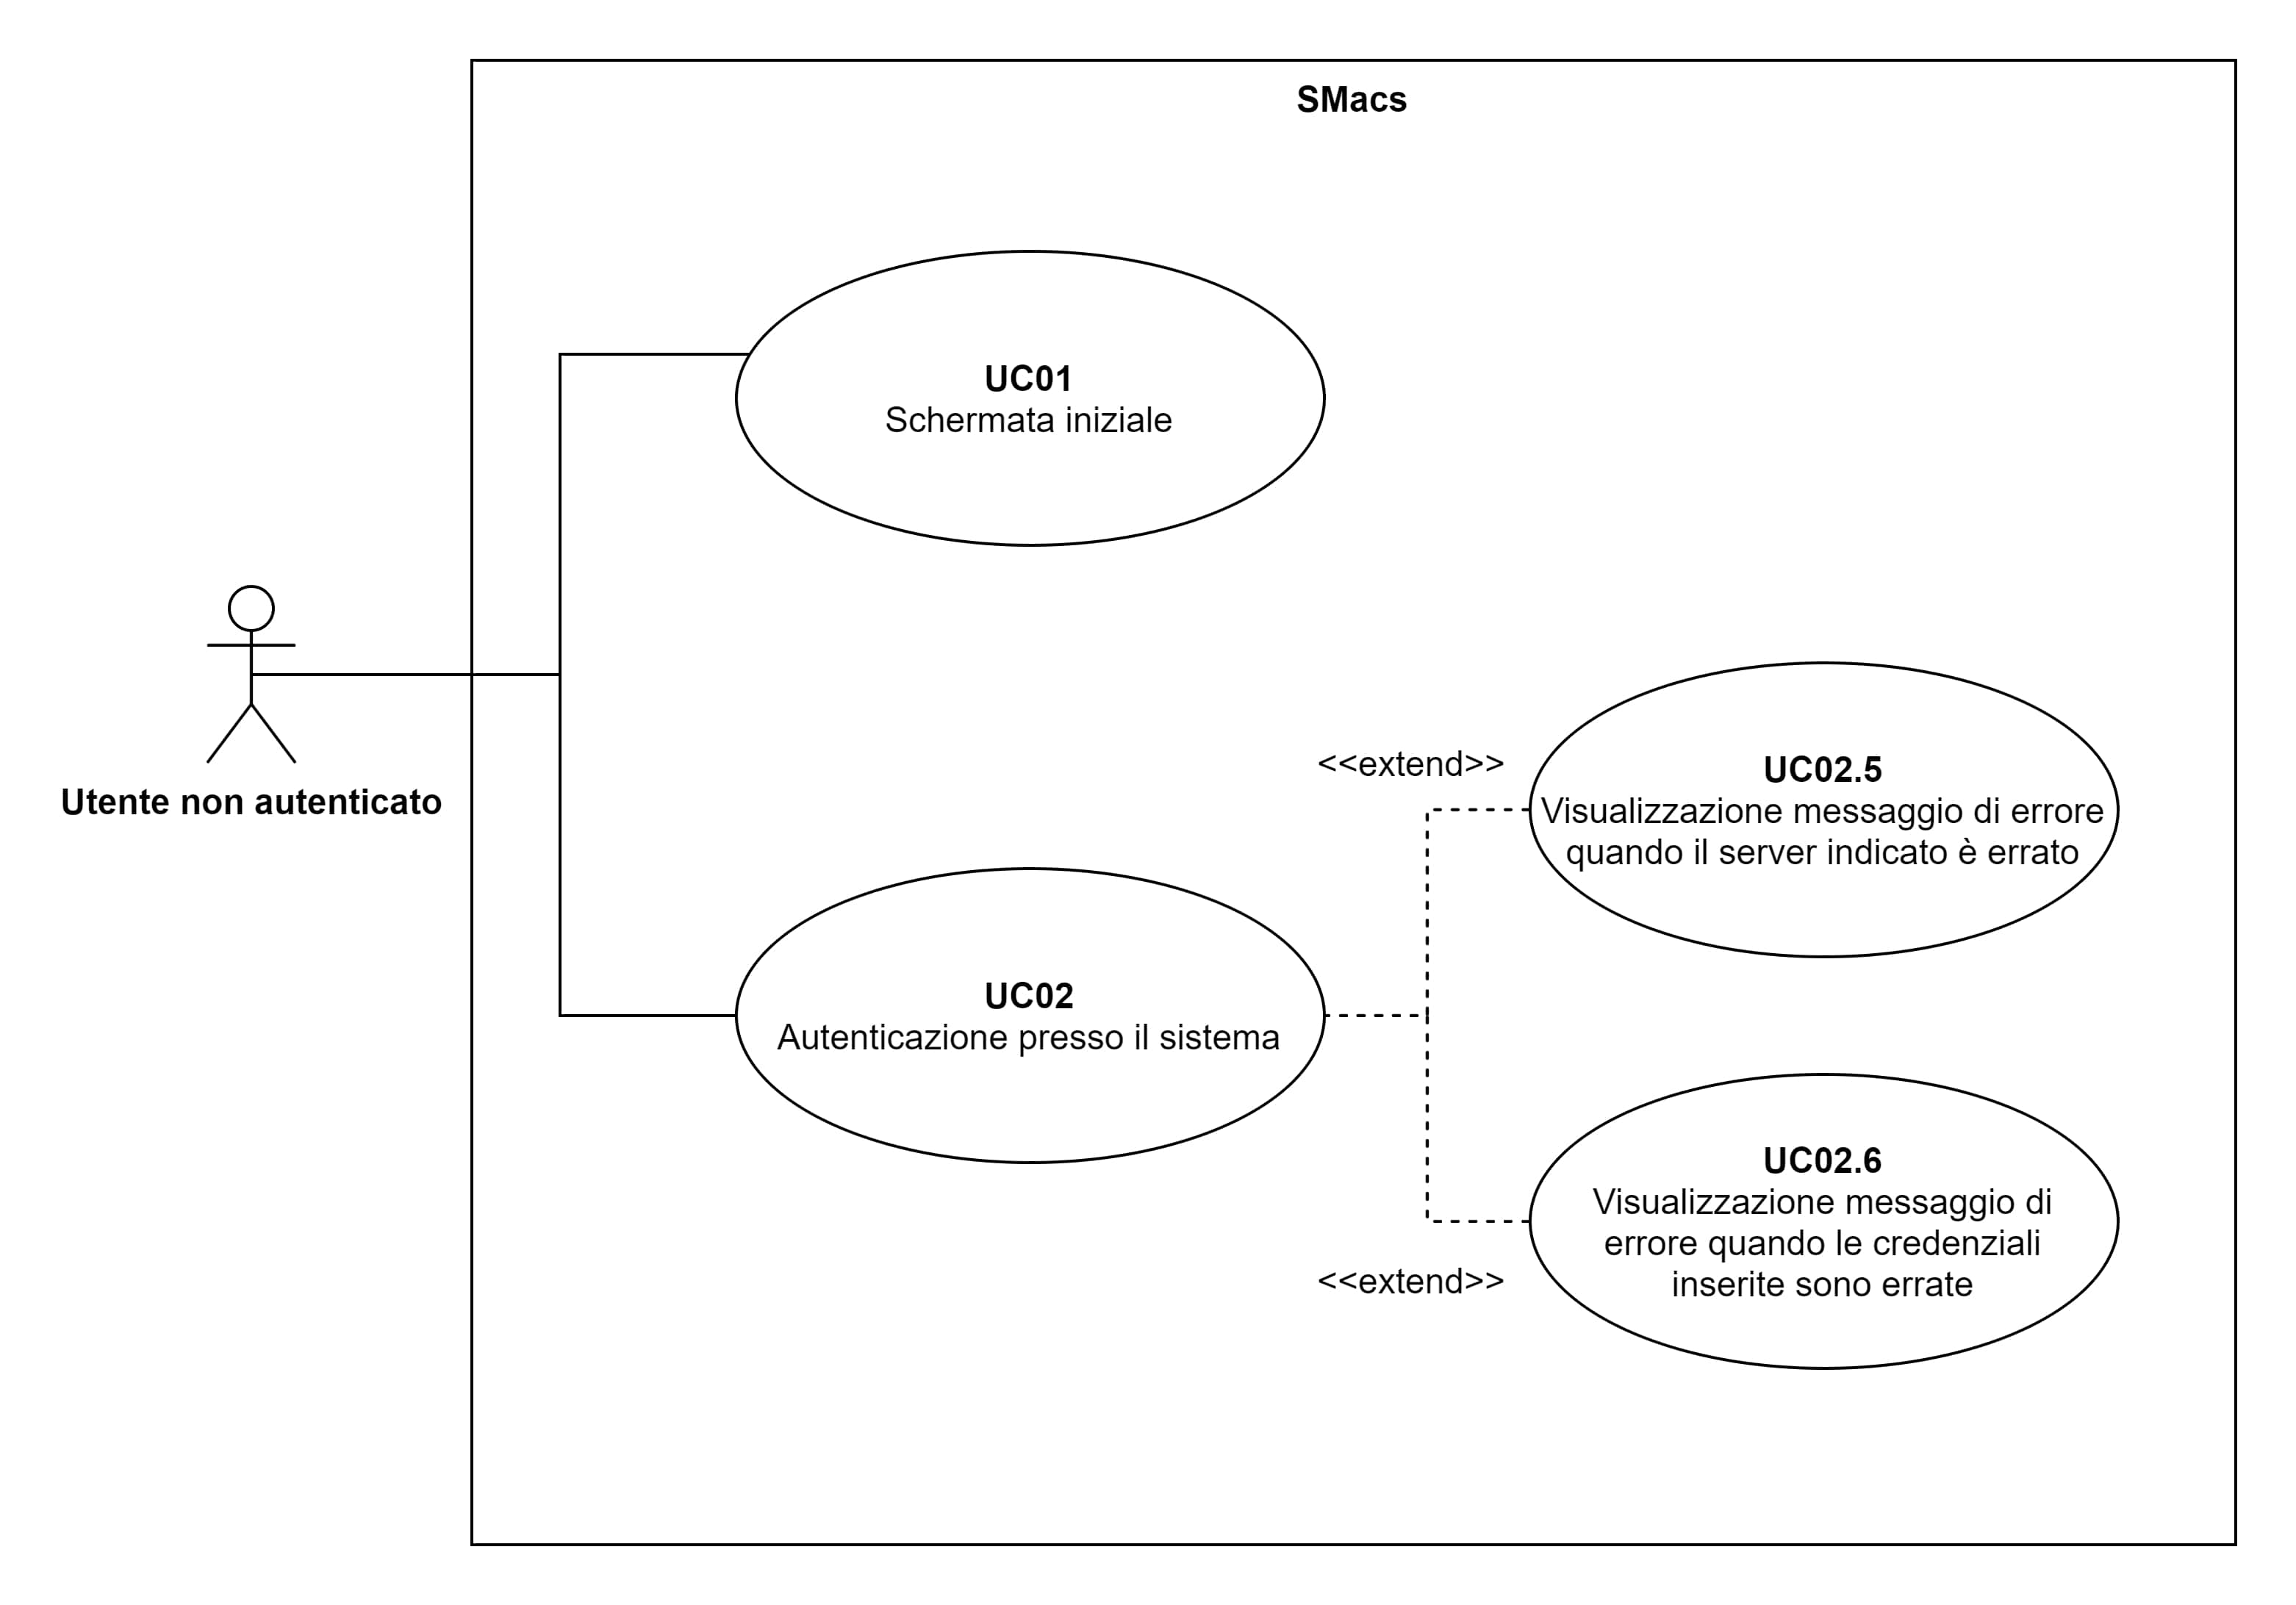
\includegraphics[width=1.0\columnwidth]{appendice-A/utente-non-autenticato} 
    \caption{SMacs - Casi d'uso dell'utente non autenticato}
\end{figure}

\begin{usecase}{01}{Schermata iniziale}
\usecaseprimaryactors{Utente non autenticato}
\usecasepre{L'utente ha appena avviato l'applicazione.}
\usecasedesc{Vengono visualizzati all'utente alcuni link per accedere a vari siti web legati all'azienda e la possibilità di aprire la pagina di accesso alle funzionalità dell'applicazione.}
\usecasepost{Viene visualizzata la schermata iniziale dell'applicazione.}
\label{uc:UC01}
\end{usecase}

\begin{figure}[!h] 
    \centering 
    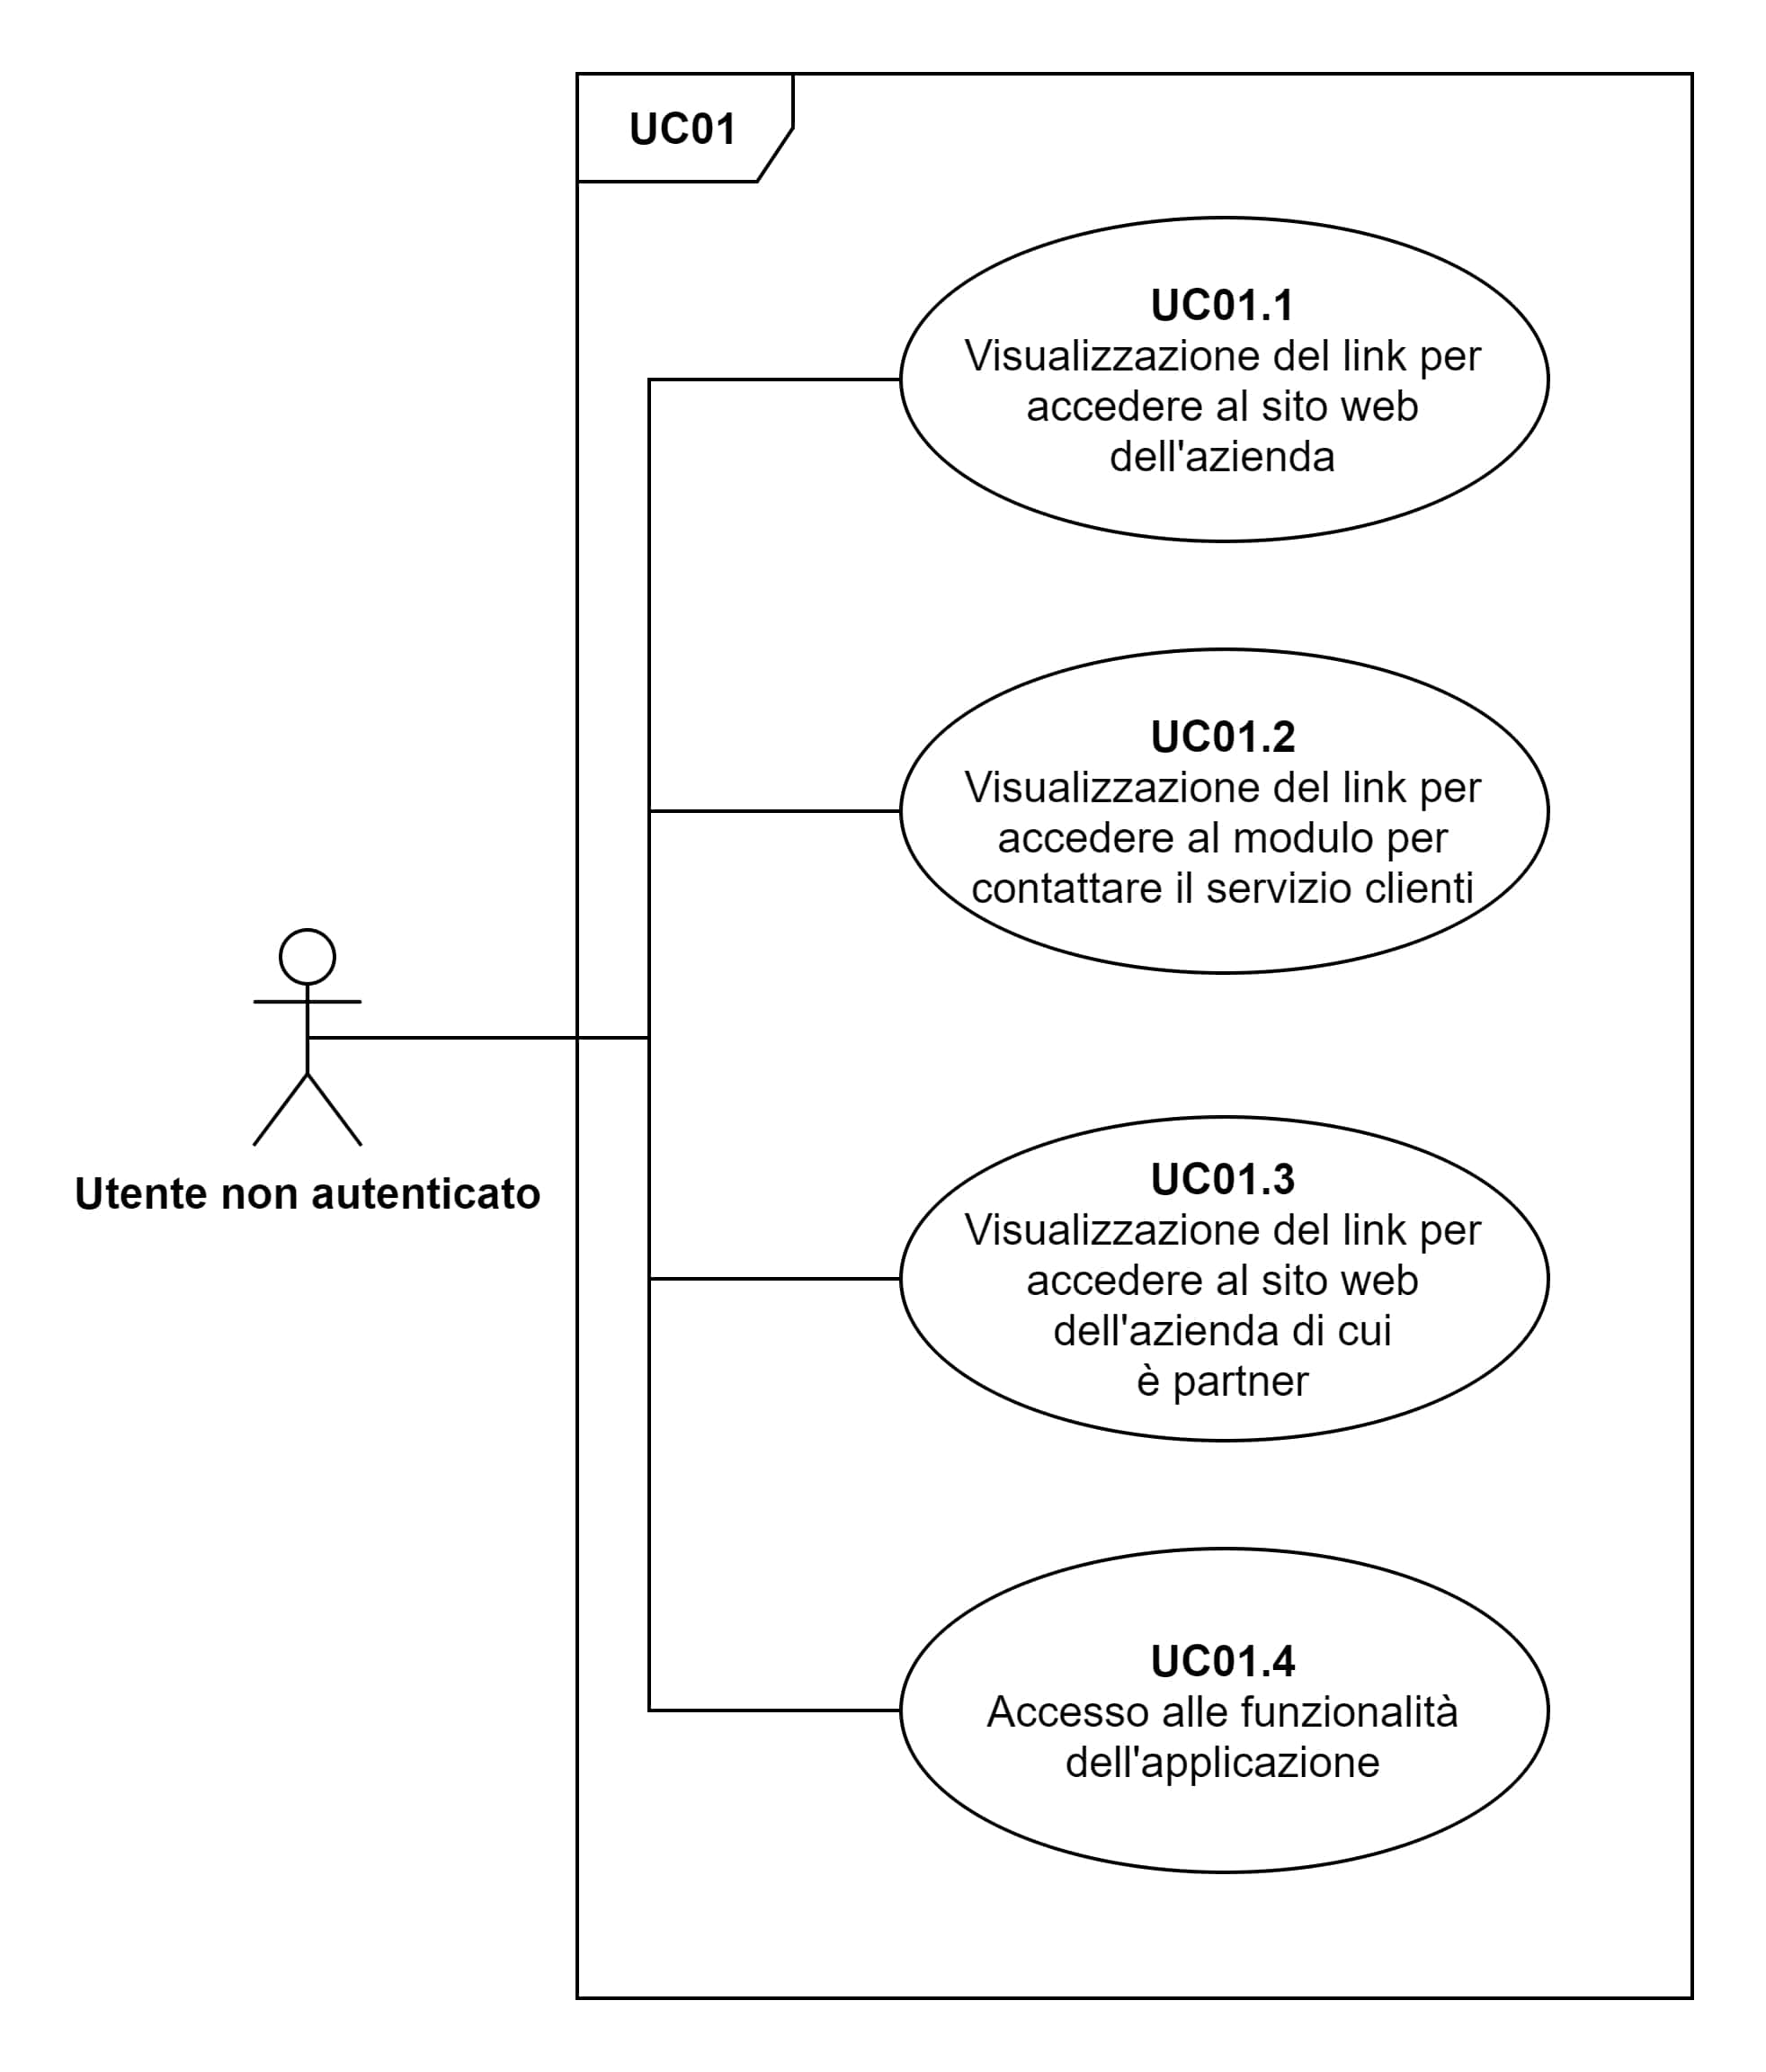
\includegraphics[width=1.0\columnwidth]{appendice-A/uc01} 
    \caption{SMacs - Sotto-casi d'uso di UC01 - Schermata iniziale}
\end{figure}

\begin{usecase}{01.1}{Visualizzazione del link per accedere al sito web dell'azienda}
\usecaseprimaryactors{Utente non autenticato}
\usecasepre{L'utente ha appena avviato l'applicazione.}
\usecasedesc{Viene visualizzato il link per accedere al sito web dell'azienda.}
\usecasepost{Viene visualizzato il link per accedere al sito web dell'azienda.}
\label{uc:UC01-1}
\end{usecase}

\begin{usecase}{01.2}{Visualizzazione del link per accedere al modulo per contattare il servizio clienti}
\usecaseprimaryactors{Utente non autenticato}
\usecasepre{L'utente ha appena avviato l'applicazione.}
\usecasedesc{Viene visualizzato il link per accedere alla pagina web per contattare il servizio clienti.}
\usecasepost{Viene visualizzato il link per accedere al modulo per contattare il servizio clienti.}
\label{uc:UC01-2}
\end{usecase}

\begin{usecase}{01.3}{Visualizzazione del link per accedere al sito web dell'azienda di cui è partner}
\usecaseprimaryactors{Utente non autenticato}
\usecasepre{L'utente ha appena avviato l'applicazione.}
\usecasedesc{Viene visualizzato il link per accedere al sito web dell'azienda di cui è partner.}
\usecasepost{Viene visualizzato il link per accedere al sito web dell'azienda di cui è partner.}
\label{uc:UC01-3}
\end{usecase}

\begin{usecase}{01.4}{Accesso alle funzionalità dell'applicazione}
\usecaseprimaryactors{Utente non autenticato}
\usecasepre{L'utente ha appena avviato l'applicazione.}
\usecasedesc{Viene visualizzato la funzionalità di accesso alla schermata di autenticazione.}
\usecasepost{Viene visualizzato la funzionalità di accesso alla schermata di autenticazione.}
\label{uc:UC01-4}
\end{usecase}

\begin{usecase}{02}{Autenticazione presso il sistema}
\usecaseprimaryactors{Utente non autenticato}
\usecasepre{L'utente ha avviato l'applicazione e ha selezionato la funzionalità di accesso nella schermata iniziale.}
\usecasedesc{L'utente può inserire il server a cui connettersi e le proprie credenziali per poter accedere presso il sistema.}
\usecasepost{L'utente si è autenticato presso il sistema.}
\usecaseext{UC02.5, UC02.6}
\label{uc:UC02}
\end{usecase}

\begin{figure}[!h] 
    \centering 
    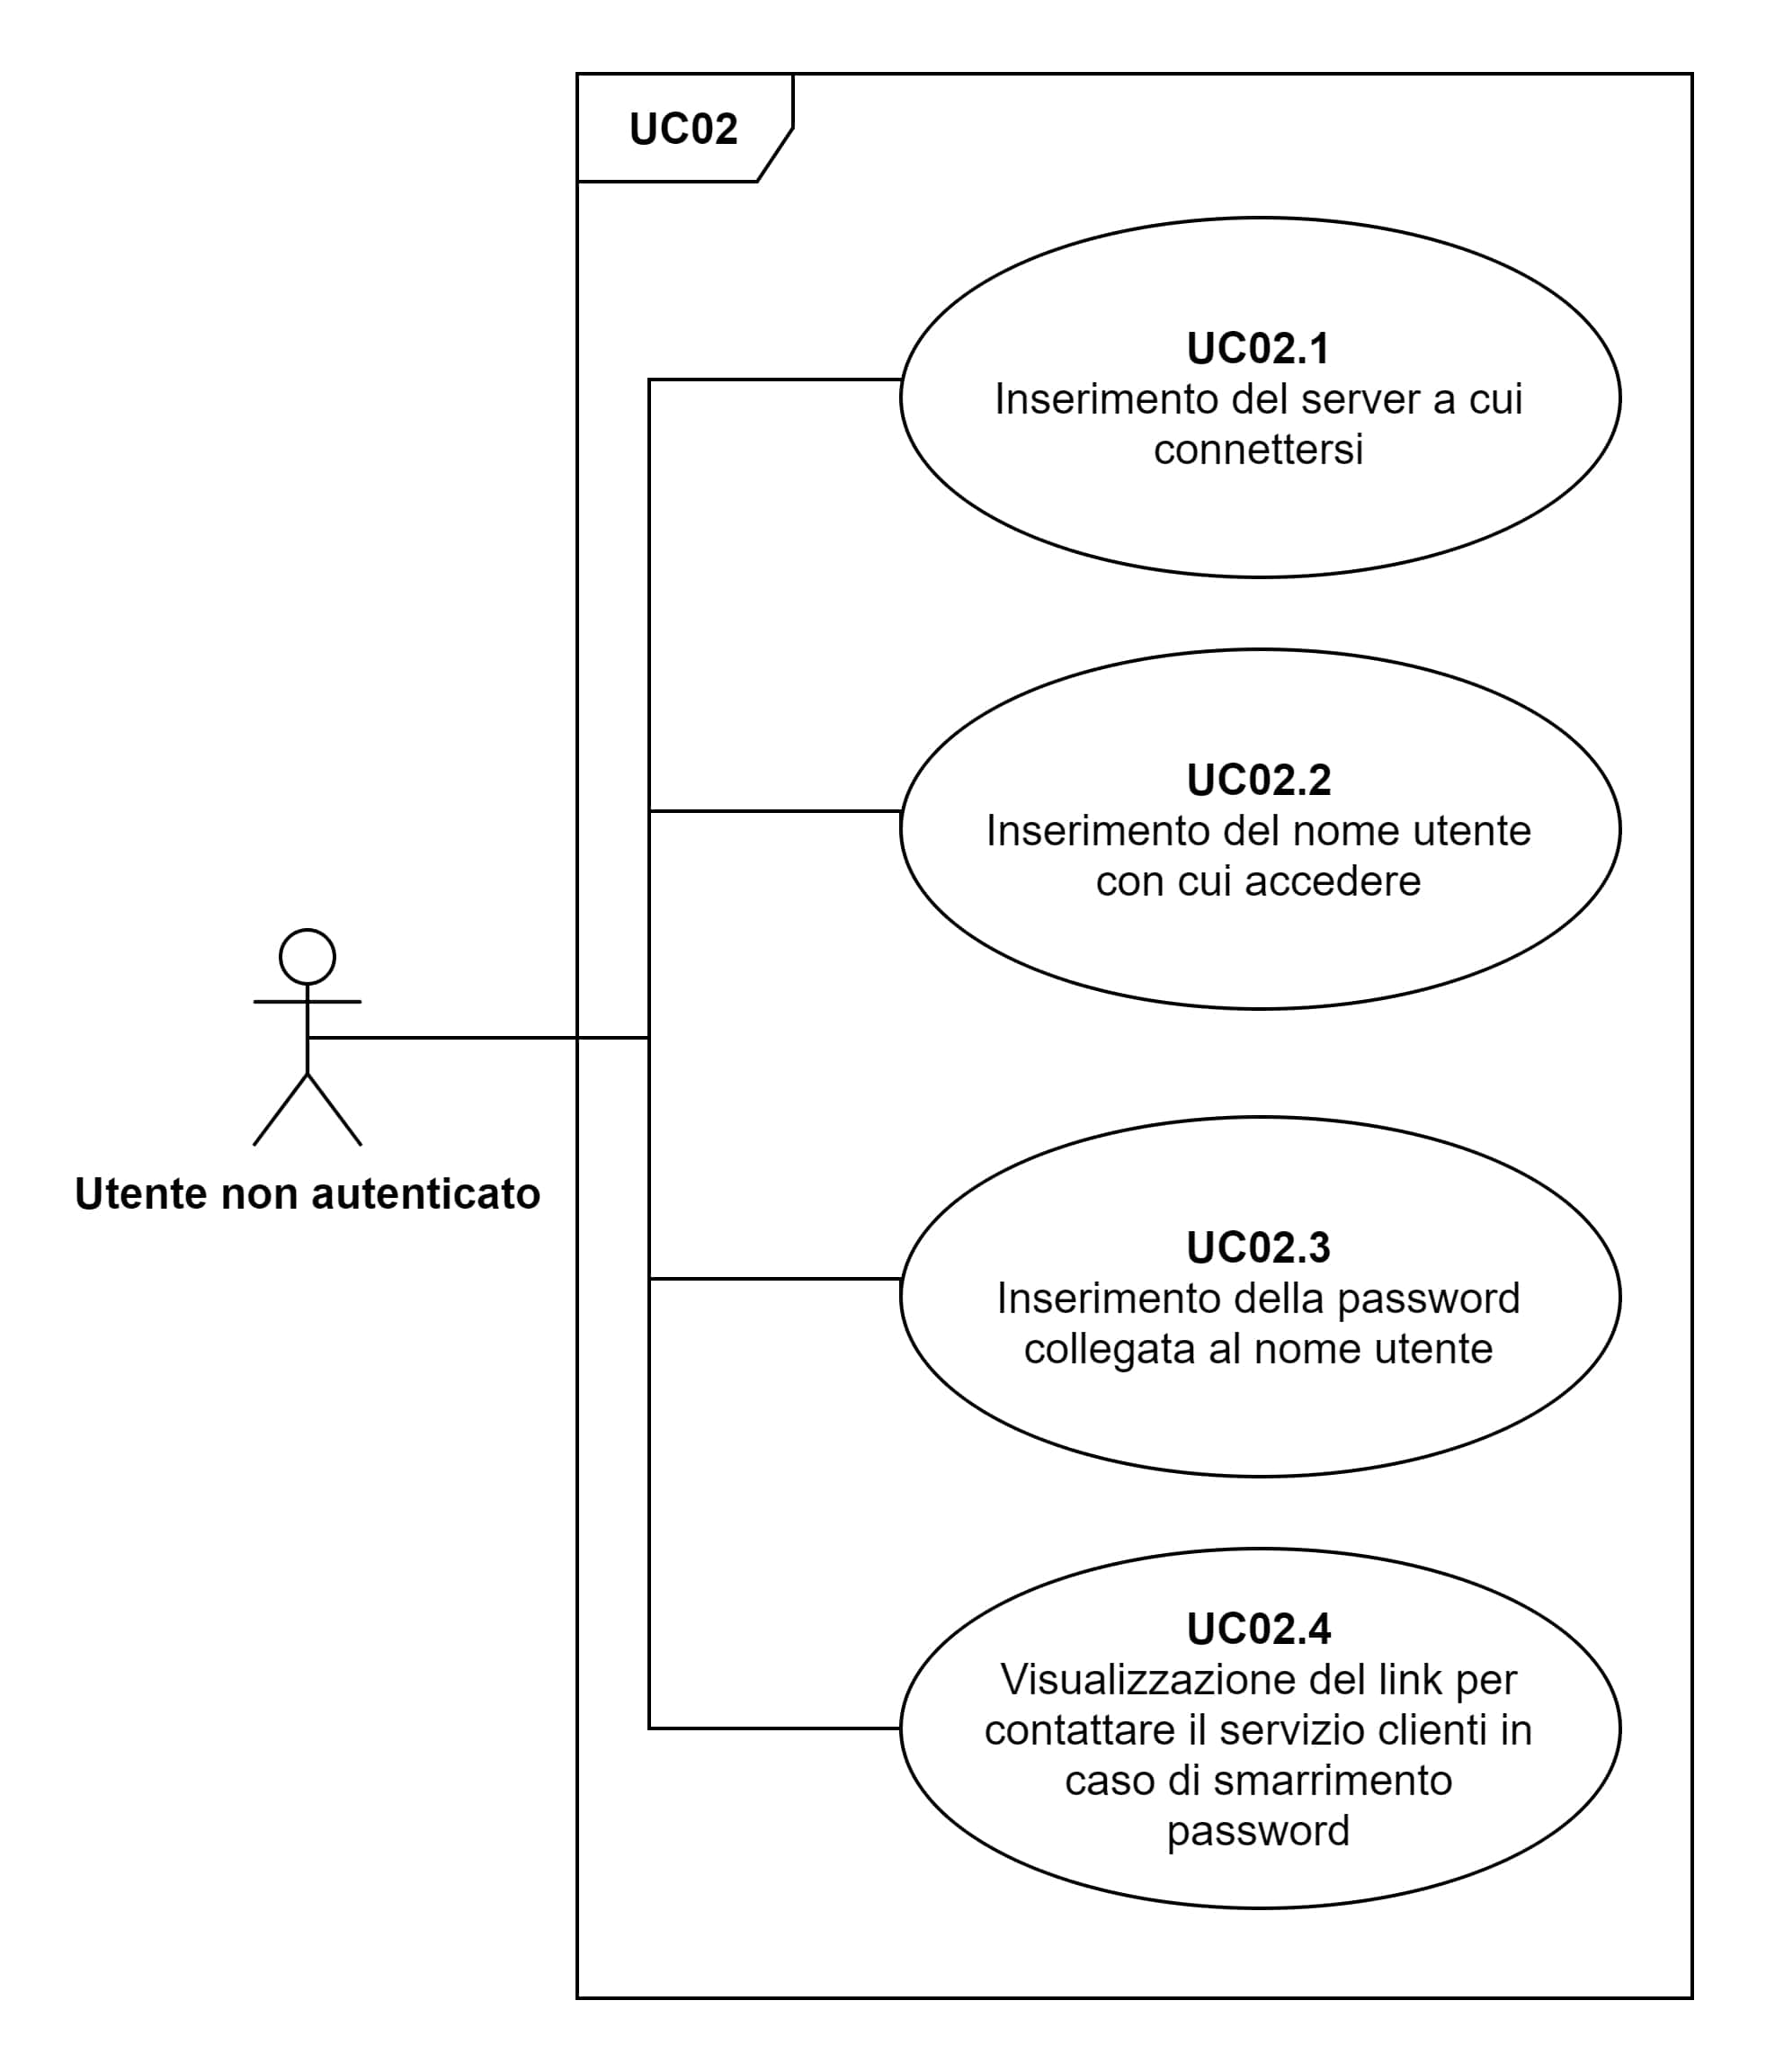
\includegraphics[width=1.0\columnwidth]{appendice-A/uc02} 
    \caption{SMacs - Sotto-casi d'uso di UC02 - Autenticazione presso il sistema}
\end{figure}

\begin{usecase}{02.1}{Inserimento del server a cui connettersi}
\usecaseprimaryactors{Utente non autenticato}
\usecasepre{L'utente ha la possibilità di inserire il server del sistema presso cui connettersi.}
\usecasedesc{L'utente può inserire il server a cui connettersi.}
\usecasepost{L'utente ha inserito il server a cui connettersi.}
\label{uc:UC02-1}
\end{usecase}

\begin{usecase}{02.2}{Inserimento del nome utente con cui accedere}
\usecaseprimaryactors{Utente non autenticato}
\usecasepre{L'utente ha la possibilità di inserire il nome utente con cui connettersi al sistema.}
\usecasedesc{L'utente può inserire il nome utente con cui connettersi al sistema.}
\usecasepost{L'utente ha inserito il proprio nome utente.}
\label{uc:UC02-2}
\end{usecase}

\begin{usecase}{02.3}{Inserimento della password collegata al nome utente}
\usecaseprimaryactors{Utente non autenticato}
\usecasepre{L'utente ha la possibilità di inserire la password con cui connettersi al sistema.}
\usecasedesc{L'utente può inserire la password con cui connettersi al sistema.}
\usecasepost{L'utente ha inserito la propria password.}
\label{uc:UC02-3}
\end{usecase}

\begin{usecase}{02.4}{Visualizzazione del link per contattare il servizio clienti in caso di smarrimento password}
\usecaseprimaryactors{Utente non autenticato}
\usecasepre{L'utente ha la possibilità di contattare il servizio clienti.}
\usecasedesc{L'utente può visualizzare il link per contattare il servizio clienti in caso di smarrimento della password.}
\usecasepost{Viene visualizzato il link per contattare il servizio clienti nel caso di smarrimento della password.}
\label{uc:UC02-4}
\end{usecase}

\begin{usecase}{02.5}{Visualizzazione messaggio di errore quando il server indicato è errato}
\usecaseprimaryactors{Utente non autenticato}
\usecasepre{L'utente ha inserito un server inesistente o a cui non è possibile connettersi.}
\usecasedesc{L'utente ha inserito un server inesistente o a cui non è possibile connettersi, di conseguenza viene visualizzato un messaggio di errore che lo informa del fatto.}
\usecasepost{Viene visualizzato un messaggio di errore che informa l'utente del fatto.}
\label{uc:UC02-5}
\end{usecase}

\begin{usecase}{02.6}{Visualizzazione messaggio di errore quando le credenziali inserite non sono valide}
\usecaseprimaryactors{Utente non autenticato}
\usecasepre{L'utente ha inserito delle credenziali errate.}
\usecasedesc{L'utente ha inserito delle credenziali errate e di conseguenza viene visualizzato un messaggio di errore che lo informa del fatto.}
\usecasepost{Viene visualizzato un messaggio di errore che informa l'utente del fatto.}
\label{uc:UC02-6}
\end{usecase}

% sicurezza che prenda tutto lo spazio disponibile
\clearpage

\begin{figure}[!h] 
    \centering 
    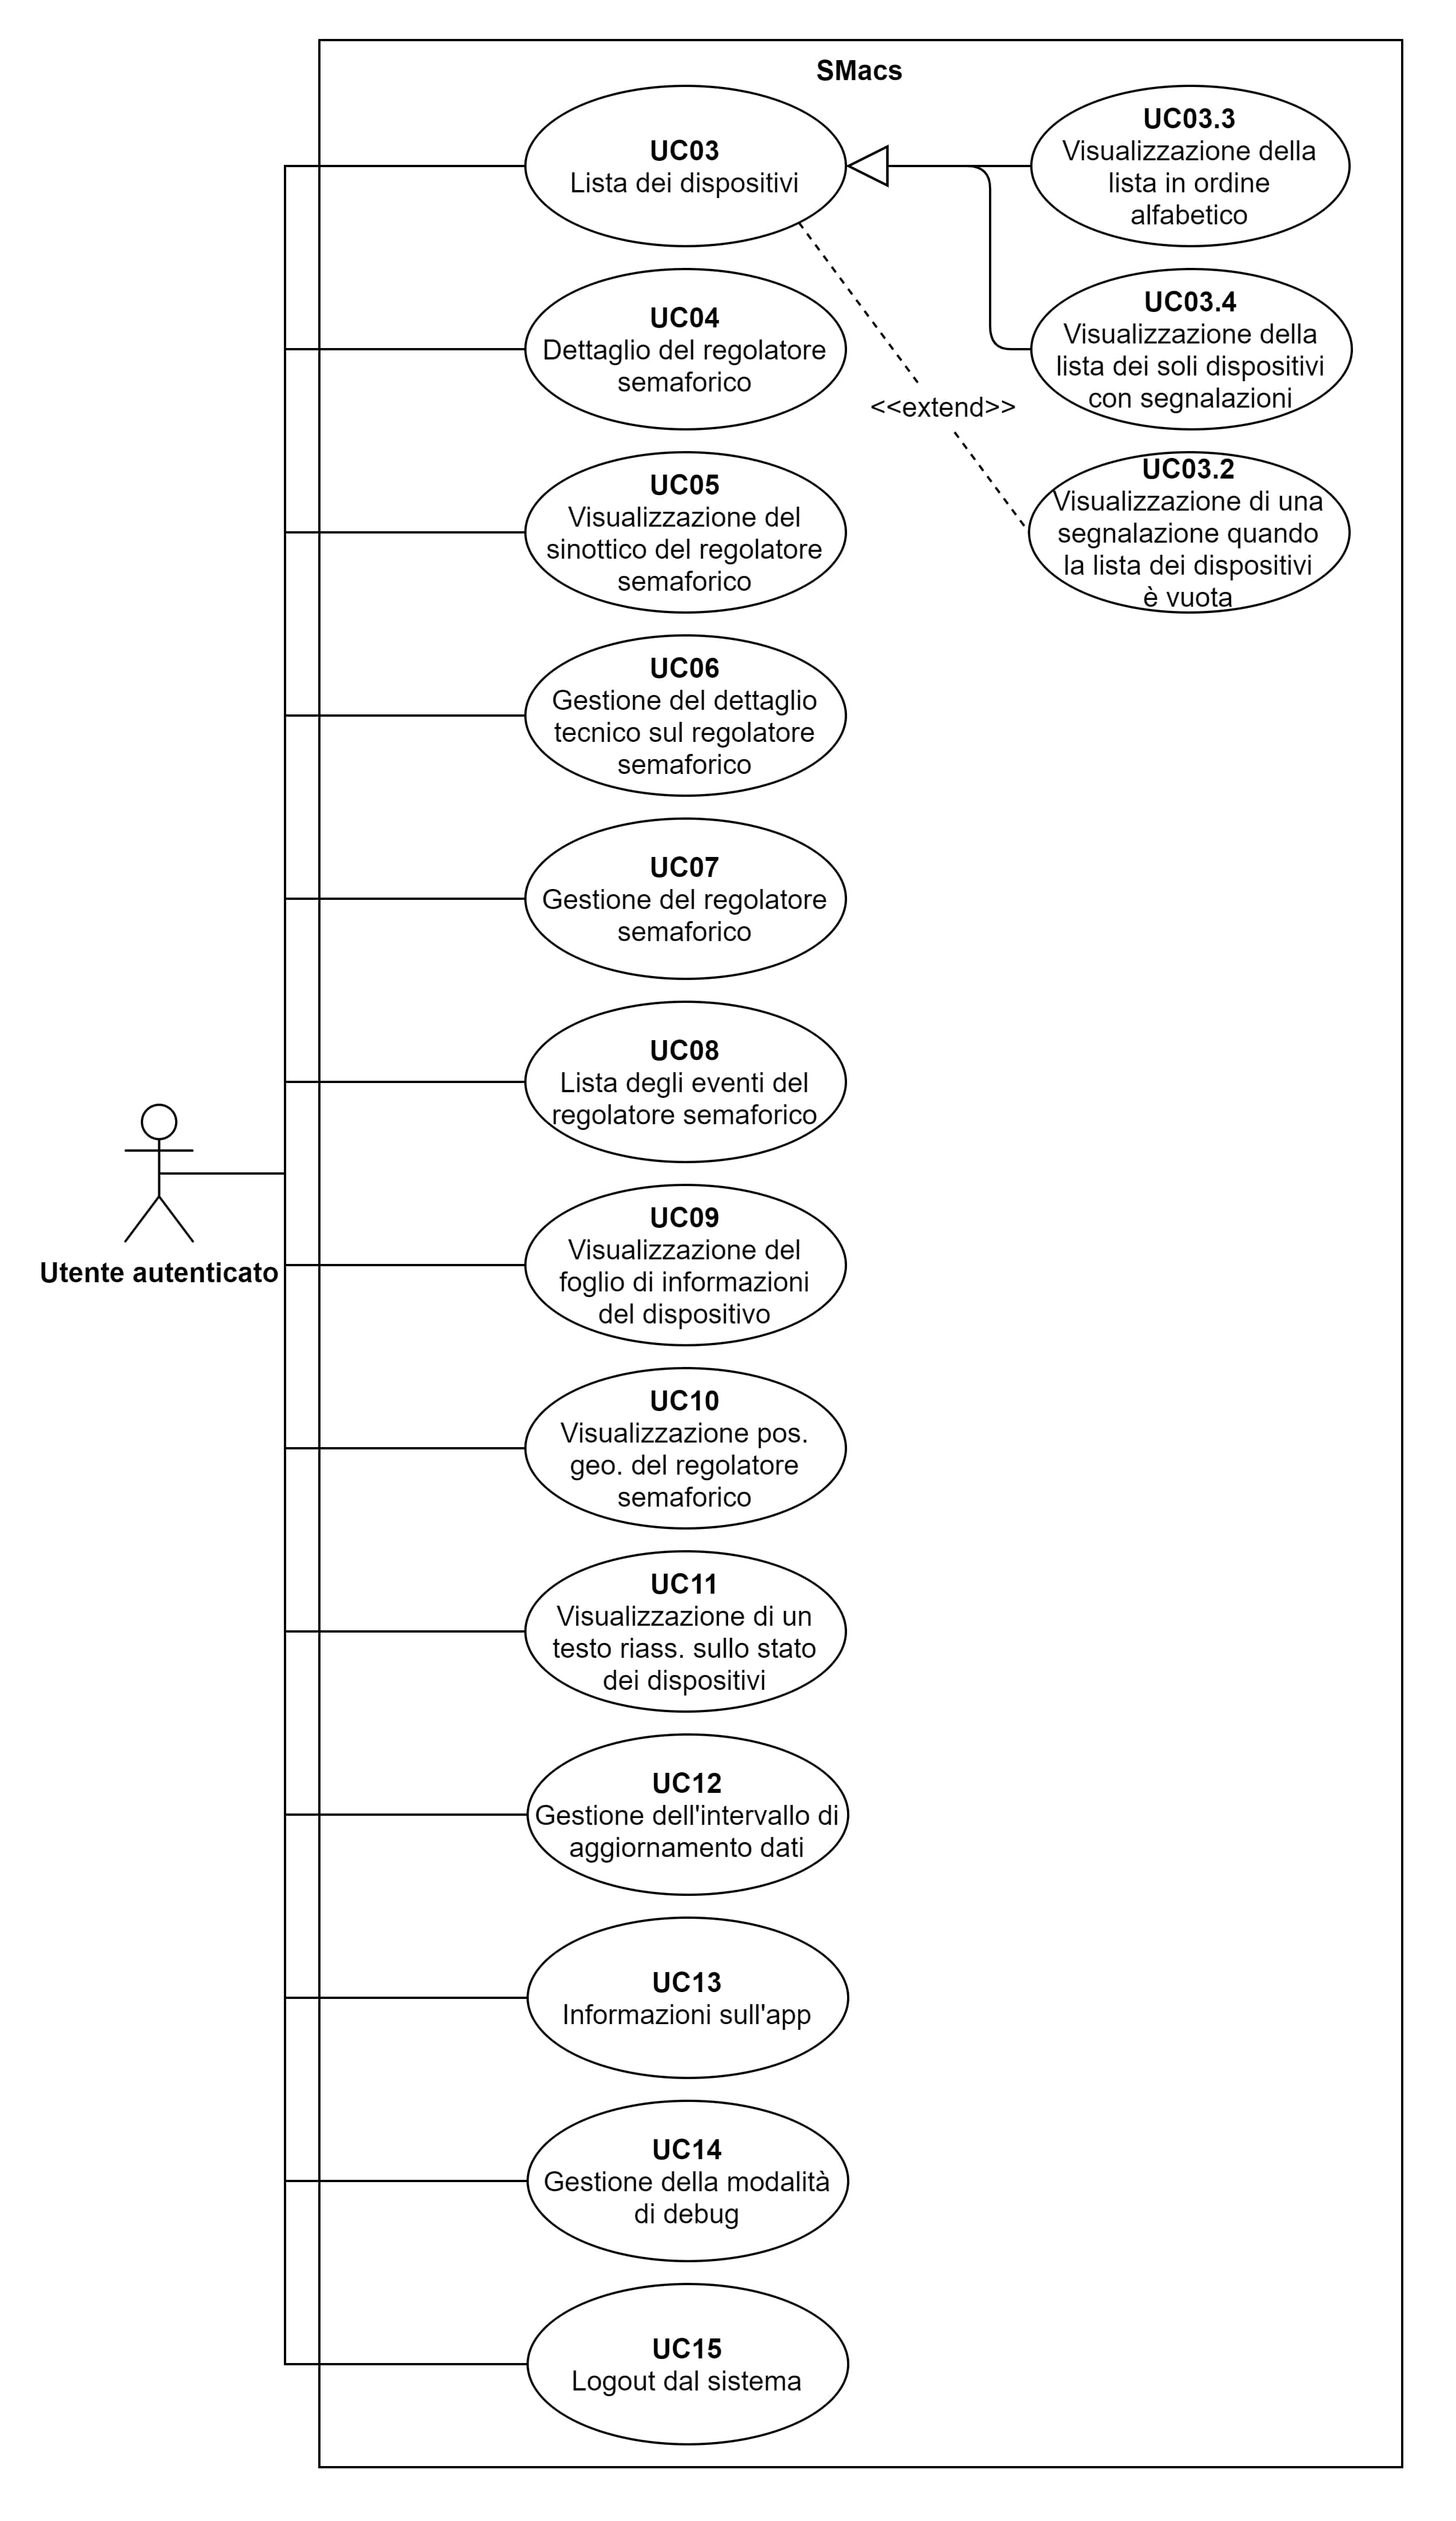
\includegraphics[height=0.94\textheight]{appendice-A/utente-autenticato} 
    \caption{SMacs - Casi d'uso dell'utente autenticato}
\end{figure}

\begin{usecase}{03}{Lista dei dispositivi}
\usecaseprimaryactors{Utente autenticato}
\usecasepre{L'utente ha accesso alla lista dei dispositivi collegati al proprio profilo.}
\usecasedesc{Viene visualizzata la lista dei dispositivi di cui l'utente può avere informazioni a riguardo.}
\usecasepost{Viene visualizzata la lista dei dispositivi di cui l'utente può avere informazioni a riguardo.}
\usecaseext{UC03.2}
\label{uc:UC03}
\end{usecase}

\begin{figure}[!h] 
    \centering 
    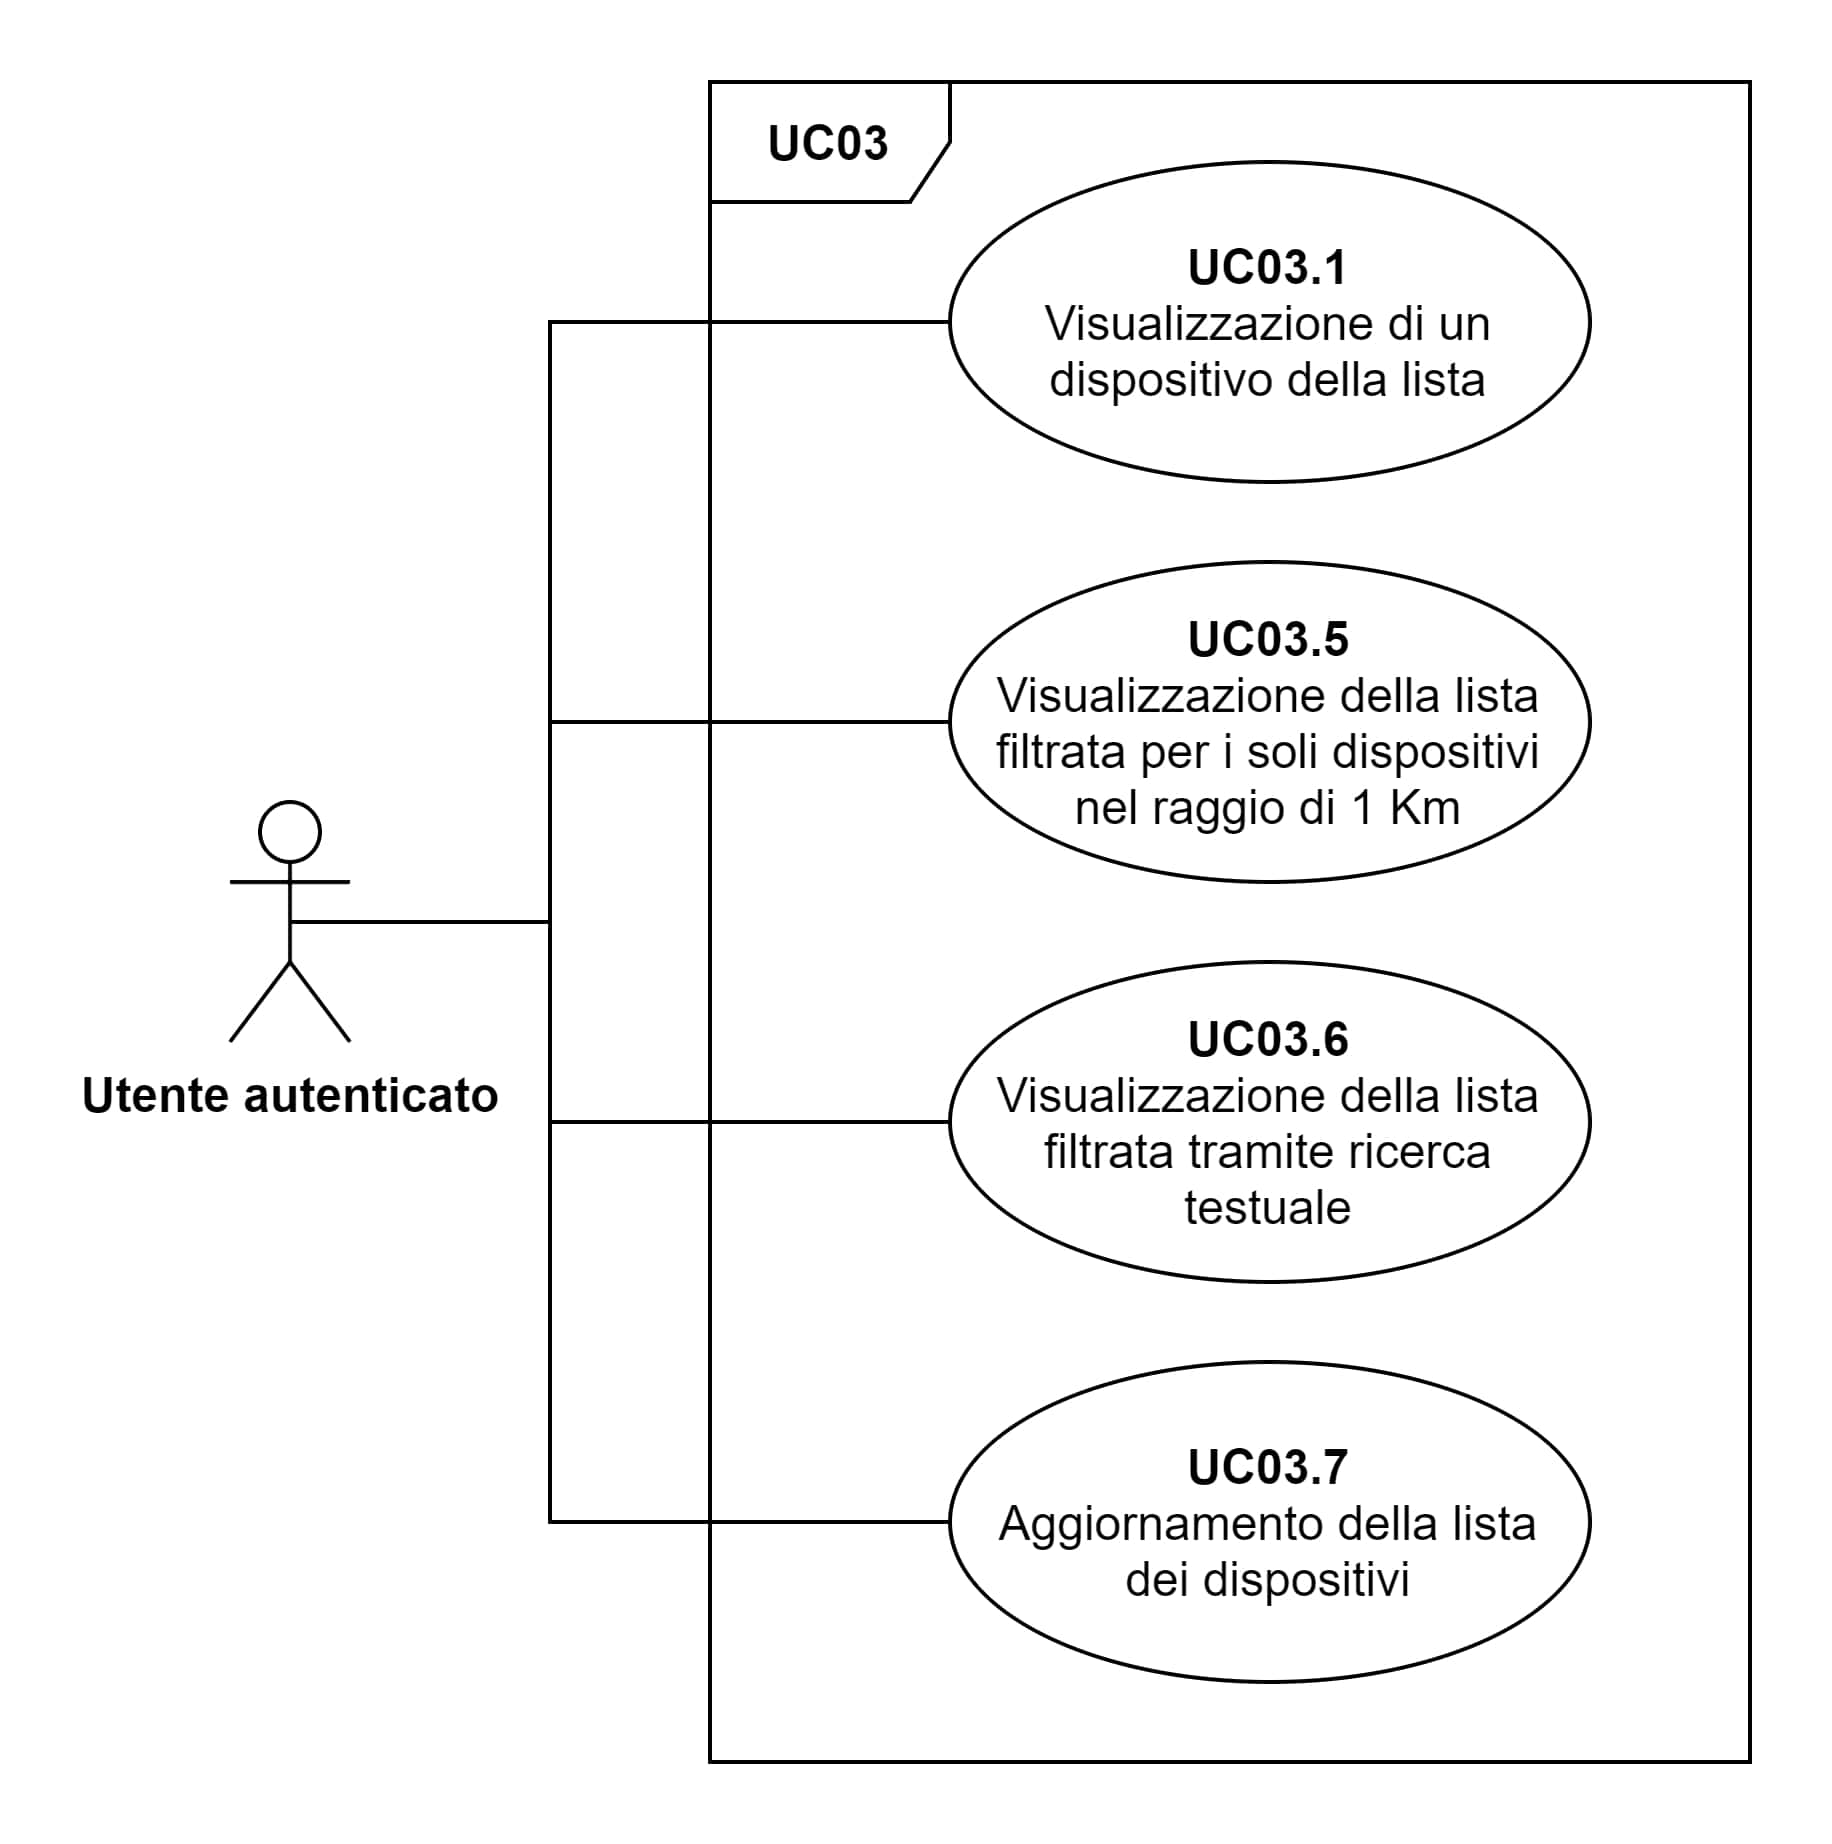
\includegraphics[width=1.0\columnwidth]{appendice-A/uc03} 
    \caption{SMacs - Sotto-casi d'uso di UC03 - Lista dei dispositivi}
\end{figure}

\begin{usecase}{03.1}{Visualizzazione di un dispositivo della lista}
\usecaseprimaryactors{Utente autenticato}
\usecasepre{L'utente sta visionando la lista dei dispositivi collegati al proprio profilo.}
\usecasedesc{Viene visualizzato un dispositivo della lista dei dispositivi collegati al profilo dell'utente, mostrandone un'icona rappresentativa e un dettaglio compatto che comprende il codice, il nome, lo stato attuale e il livello massimo di segnalazione attuale. Inoltre, viene mostrata la data di ultimo aggiornamento.}
\usecasepost{Viene visualizzato un dispositivo della lista dei dispositivi collegati al profilo dell'utente, mostrandone un dettaglio compatto.}
\label{uc:UC03-1}
\end{usecase}

\begin{usecase}{03.2}{Visualizzazione di una segnalazione quando la lista dei dispositivi è vuota}
\usecaseprimaryactors{Utente autenticato}
\usecasepre{L'utente sta visionando la lista dei dispositivi collegati al proprio profilo ma è vuota.}
\usecasedesc{L'utente sta visionando la lista dei dispositivi collegati al proprio profilo ma è vuota, quindi viene avvisato mediante un messaggio,}
\usecasepost{Viene visualizzato un messaggio che avvisa l'utente che la lista è vuota.}
\label{uc:UC03-2}
\end{usecase}

\begin{usecase}{03.3}{Visualizzazione della lista in ordine alfabetico}
\usecaseprimaryactors{Utente autenticato}
\usecasepre{L'utente sta visionando la lista dei dispositivi collegati al proprio profilo.}
\usecasedesc{Viene visualizzata la lista dei dispositivi di cui l'utente può avere informazioni a riguardo in ordine alfabetico (corrisponde all'opzione di default).}
\usecasepost{Viene visualizzata la lista dei dispositivi di cui l'utente può avere informazioni a riguardo in ordine alfabetico.}
\usecasegen{UC03}
\label{uc:UC03-3}
\end{usecase}

\begin{usecase}{03.4}{Visualizzazione della lista dei soli dispositivi con segnalazioni}
\usecaseprimaryactors{Utente autenticato}
\usecasepre{L'utente sta visionando la lista dei dispositivi collegati al proprio profilo.}
\usecasedesc{Viene visualizzata la lista dei dispositivi con segnalazioni (di malfunzionamento) di cui l'utente può avere informazioni a riguardo.}
\usecasepost{Viene visualizzata la lista dei dispositivi con segnalazioni (di malfunzionamento) di cui l'utente può avere informazioni a riguardo.}
\usecasegen{UC03}
\label{uc:UC03-4}
\end{usecase}

\begin{usecase}{03.5}{Visualizzazione della lista filtrata per i soli dispositivi nel raggio di 1 Km}
\usecaseprimaryactors{Utente autenticato}
\usecasepre{L'utente sta visionando la lista dei dispositivi collegati al proprio profilo.}
\usecasedesc{Viene visualizzata la lista dei dispositivi entro il raggio di 1 Km dalla posizione geografica attuale dell'utente di cui l'utente può avere informazioni a riguardo.}
\usecasepost{Viene visualizzata la lista dei dispositivi entro il raggio di 1 Km dalla posizione geografica attuale dell'utente di cui l'utente può avere informazioni a riguardo.}
\label{uc:UC03-5}
\end{usecase}

\begin{usecase}{03.6}{Visualizzazione della lista filtrata tramite ricerca testuale}
\usecaseprimaryactors{Utente autenticato}
\usecasepre{L'utente sta visionando la lista dei dispositivi collegati al proprio profilo.}
\usecasedesc{Viene visualizzata la lista dei dispositivi in base alla ricerca inoltrata di cui l'utente può avere informazioni a riguardo.}
\usecasepost{Viene visualizzata la lista dei dispositivi in base alla ricerca inoltrata di cui l'utente può avere informazioni a riguardo.}
\label{uc:UC03-6}
\end{usecase}

\begin{usecase}{03.7}{Aggiornamento della lista dei dispositivi}
\usecaseprimaryactors{Utente autenticato}
\usecasepre{L'utente sta visionando la lista dei dispositivi collegati al proprio profilo.}
\usecasedesc{L'utente seleziona la funzionalità di aggiornamento e viene aggiornata la lista dei dispositivi di cui l'utente può avere informazioni a riguardo ottenendone una nuova copia dal sistema.}
\usecasepost{L'utente seleziona la funzionalità di aggiornamento e viene aggiornata la lista dei dispositivi di cui l'utente può avere informazioni a riguardo ottenendone una nuova copia dal sistema.}
\label{uc:UC03-7}
\end{usecase}

\begin{usecase}{04}{Dettaglio del regolatore semaforico}
\usecaseprimaryactors{Utente autenticato}
\usecasepre{L'utente sta visionando la lista dei dispositivi collegati al proprio profilo e seleziona un regolatore semaforico dalla lista.}
\usecasedesc{Vengono visualizzati informazioni dettagliate sullo stato del regolatore semaforico.}
\usecasepost{Vengono visualizzati informazioni dettagliate sullo stato del regolatore semaforico.}
\label{uc:UC04}
\end{usecase}

\begin{figure}[!h] 
    \centering 
    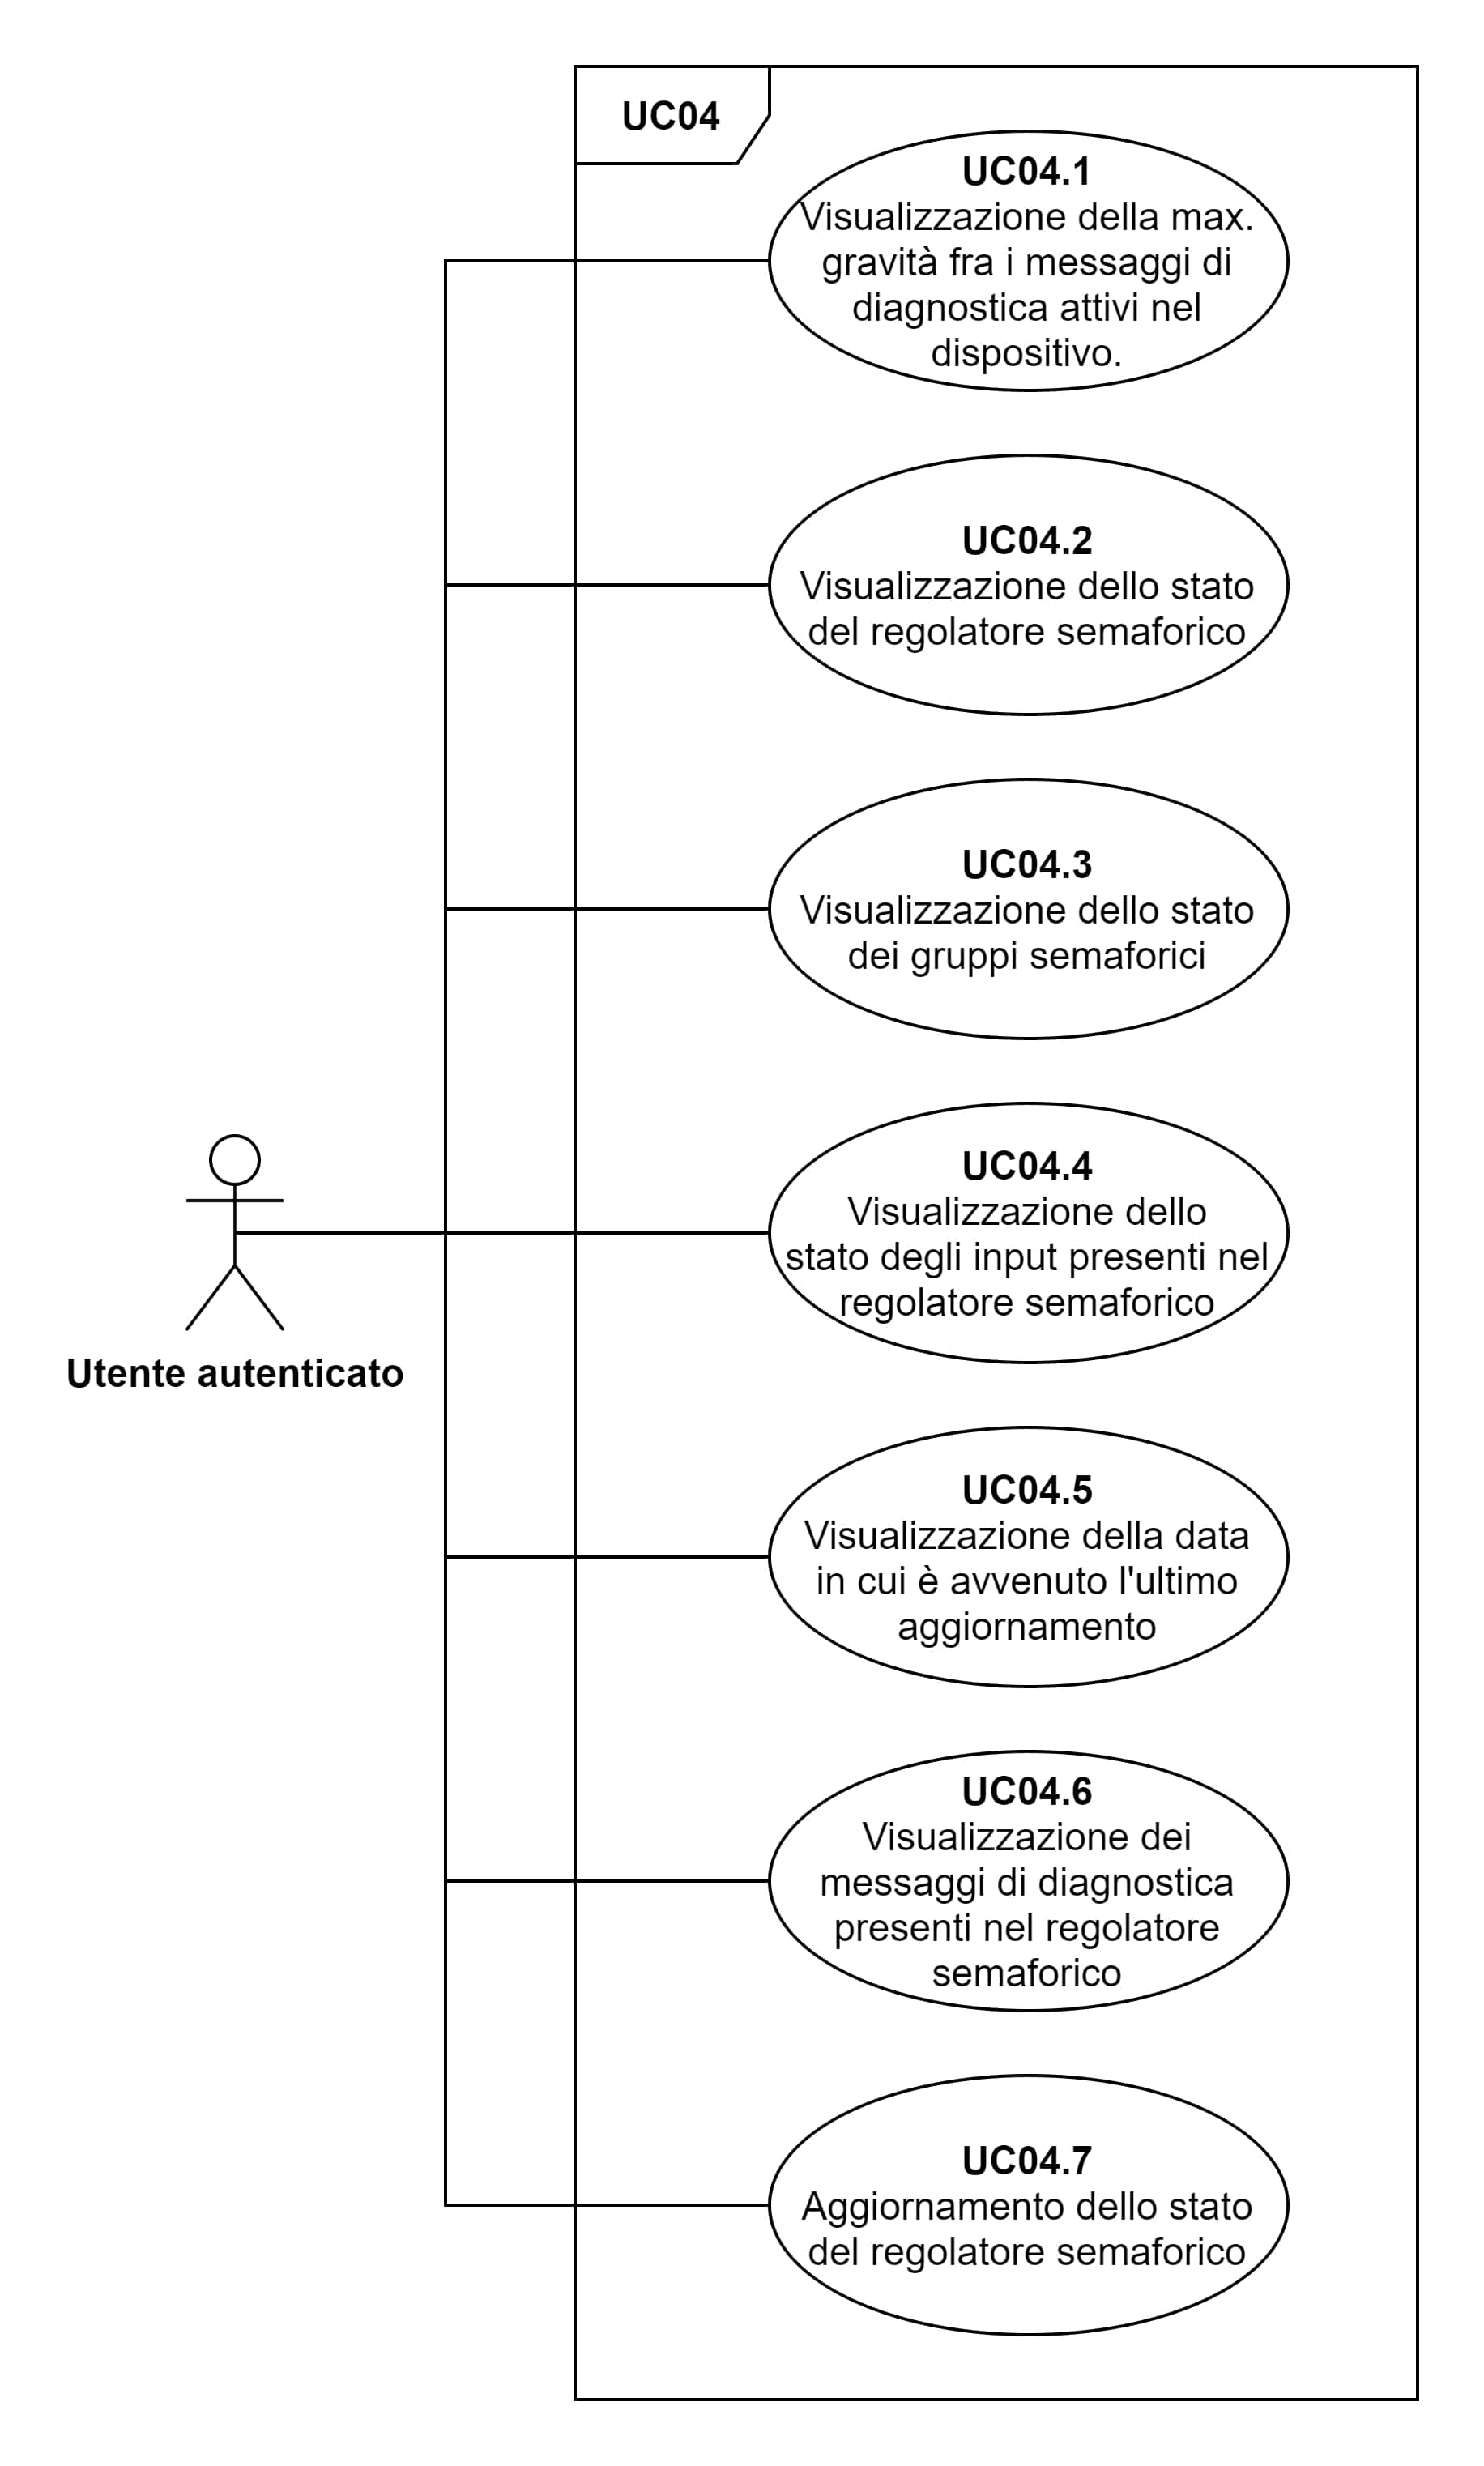
\includegraphics[width=0.9\columnwidth]{appendice-A/uc04} 
    \caption{SMacs - Sotto-casi d'uso di UC04 - Dettaglio del regolatore semaforico}
\end{figure}

\begin{usecase}{04.1}{Visualizzazione della massima gravità fra i messaggi di diagnostica attivi nel dispositivo.}
\usecaseprimaryactors{Utente autenticato}
\usecasepre{L'utente sta visionando il dettaglio del regolatore semaforico selezionato dalla lista.}
\usecasedesc{Viene visualizzato lo stato di diagnostica del regolatore semaforico.}
\usecasepost{Viene visualizzato lo stato di diagnostica del regolatore semaforico.}
\label{uc:UC04-1}
\end{usecase}

\begin{usecase}{04.2}{Visualizzazione dello stato del regolatore semaforico}
\usecaseprimaryactors{Utente autenticato}
\usecasepre{L'utente sta visionando il dettaglio del regolatore semaforico selezionato dalla lista.}
\usecasedesc{Viene visualizzato lo stato del regolatore semaforico (funzione, modalità, livello, step, tempo).}
\usecasepost{Viene visualizzato lo stato del regolatore semaforico (funzione, modalità, livello, step, tempo).}
\label{uc:UC04-2}
\end{usecase}

\begin{usecase}{04.3}{Visualizzazione dello stato dei gruppi semaforici}
\usecaseprimaryactors{Utente autenticato}
\usecasepre{L'utente sta visionando il dettaglio del regolatore semaforico selezionato dalla lista.}
\usecasedesc{Viene visualizzato lo stato dei gruppi semaforici.}
\usecasepost{Viene visualizzato lo stato dei gruppi semaforici.}
\label{uc:UC04-3}
\end{usecase}

\begin{usecase}{04.4}{Visualizzazione dello stato degli input presenti nel regolatore semaforico}
\usecaseprimaryactors{Utente autenticato}
\usecasepre{L'utente sta visionando il dettaglio del regolatore semaforico selezionato dalla lista.}
\usecasedesc{Viene visualizzato lo stato degli input presenti nel regolatore semaforico.}
\usecasepost{Viene visualizzato lo stato degli input presenti nel regolatore semaforico.}
\label{uc:UC04-4}
\end{usecase}

\begin{usecase}{04.5}{Visualizzazione della data in cui è avvenuto l'ultimo aggiornamento}
\usecaseprimaryactors{Utente autenticato}
\usecasepre{L'utente sta visionando il dettaglio del regolatore semaforico selezionato dalla lista.}
\usecasedesc{Viene visualizzata la data dell'ultimo aggiornamento del dettaglio del regolatore semaforico.}
\usecasepost{Viene visualizzata la data dell'ultimo aggiornamento del dettaglio del regolatore semaforico.}
\label{uc:UC04-5}
\end{usecase}

\begin{usecase}{04.6}{Visualizzazione dei messaggi di diagnostica presenti nel regolatore semaforico}
\usecaseprimaryactors{Utente autenticato}
\usecasepre{L'utente sta visionando il dettaglio del regolatore semaforico selezionato dalla lista.}
\usecasedesc{Vengono visualizzati i messaggi di diagnostica presenti nel regolatore semaforico.}
\usecasepost{Vengono visualizzati i messaggi di diagnostica presenti nel regolatore semaforico.}
\label{uc:UC04-6}
\end{usecase}

\begin{usecase}{04.7}{Aggiornamento dello stato del regolatore semaforico}
\usecaseprimaryactors{Utente autenticato}
\usecasepre{L'utente sta visionando il dettaglio del regolatore semaforico selezionato dalla lista.}
\usecasedesc{L'utente seleziona la funzionalità di aggiornamento e viene aggiornato lo stato del regolatore semaforico.}
\usecasepost{L'utente seleziona la funzionalità di aggiornamento e viene aggiornato lo stato del regolatore semaforico.}
\label{uc:UC04-7}
\end{usecase}

\begin{usecase}{05}{Visualizzazione del sinottico del regolatore semaforico}
\usecaseprimaryactors{Utente autenticato}
\usecasepre{L'utente sta visionando il dettaglio del regolatore semaforico selezionato dalla lista.}
\usecasedesc{L'utente ha selezionato la funzionalità di visualizzazione del sinottico del regolatore semaforico.}
\usecasepost{L'utente ha selezionato la funzionalità di visualizzazione del sinottico del regolatore semaforico, che presenta una vista d'insieme del tratto di strada in cui è posizionato il regolatore semaforico.}
\label{uc:UC05}
\end{usecase}

\begin{usecase}{06}{Gestione del dettaglio tecnico sul regolatore semaforico}
\usecaseprimaryactors{Utente autenticato}
\usecasepre{L'utente sta visionando il dettaglio del regolatore semaforico selezionato dalla lista.}
\usecasedesc{L'utente può gestire il dettaglio tecnico del regolatore semaforico, visualizzandolo e aggiungendo note.}
\usecasepost{L'utente può gestire il dettaglio tecnico del regolatore semaforico, visualizzandolo e aggiungendo note.}
\label{uc:UC06}
\end{usecase}

\begin{figure}[!h] 
    \centering 
    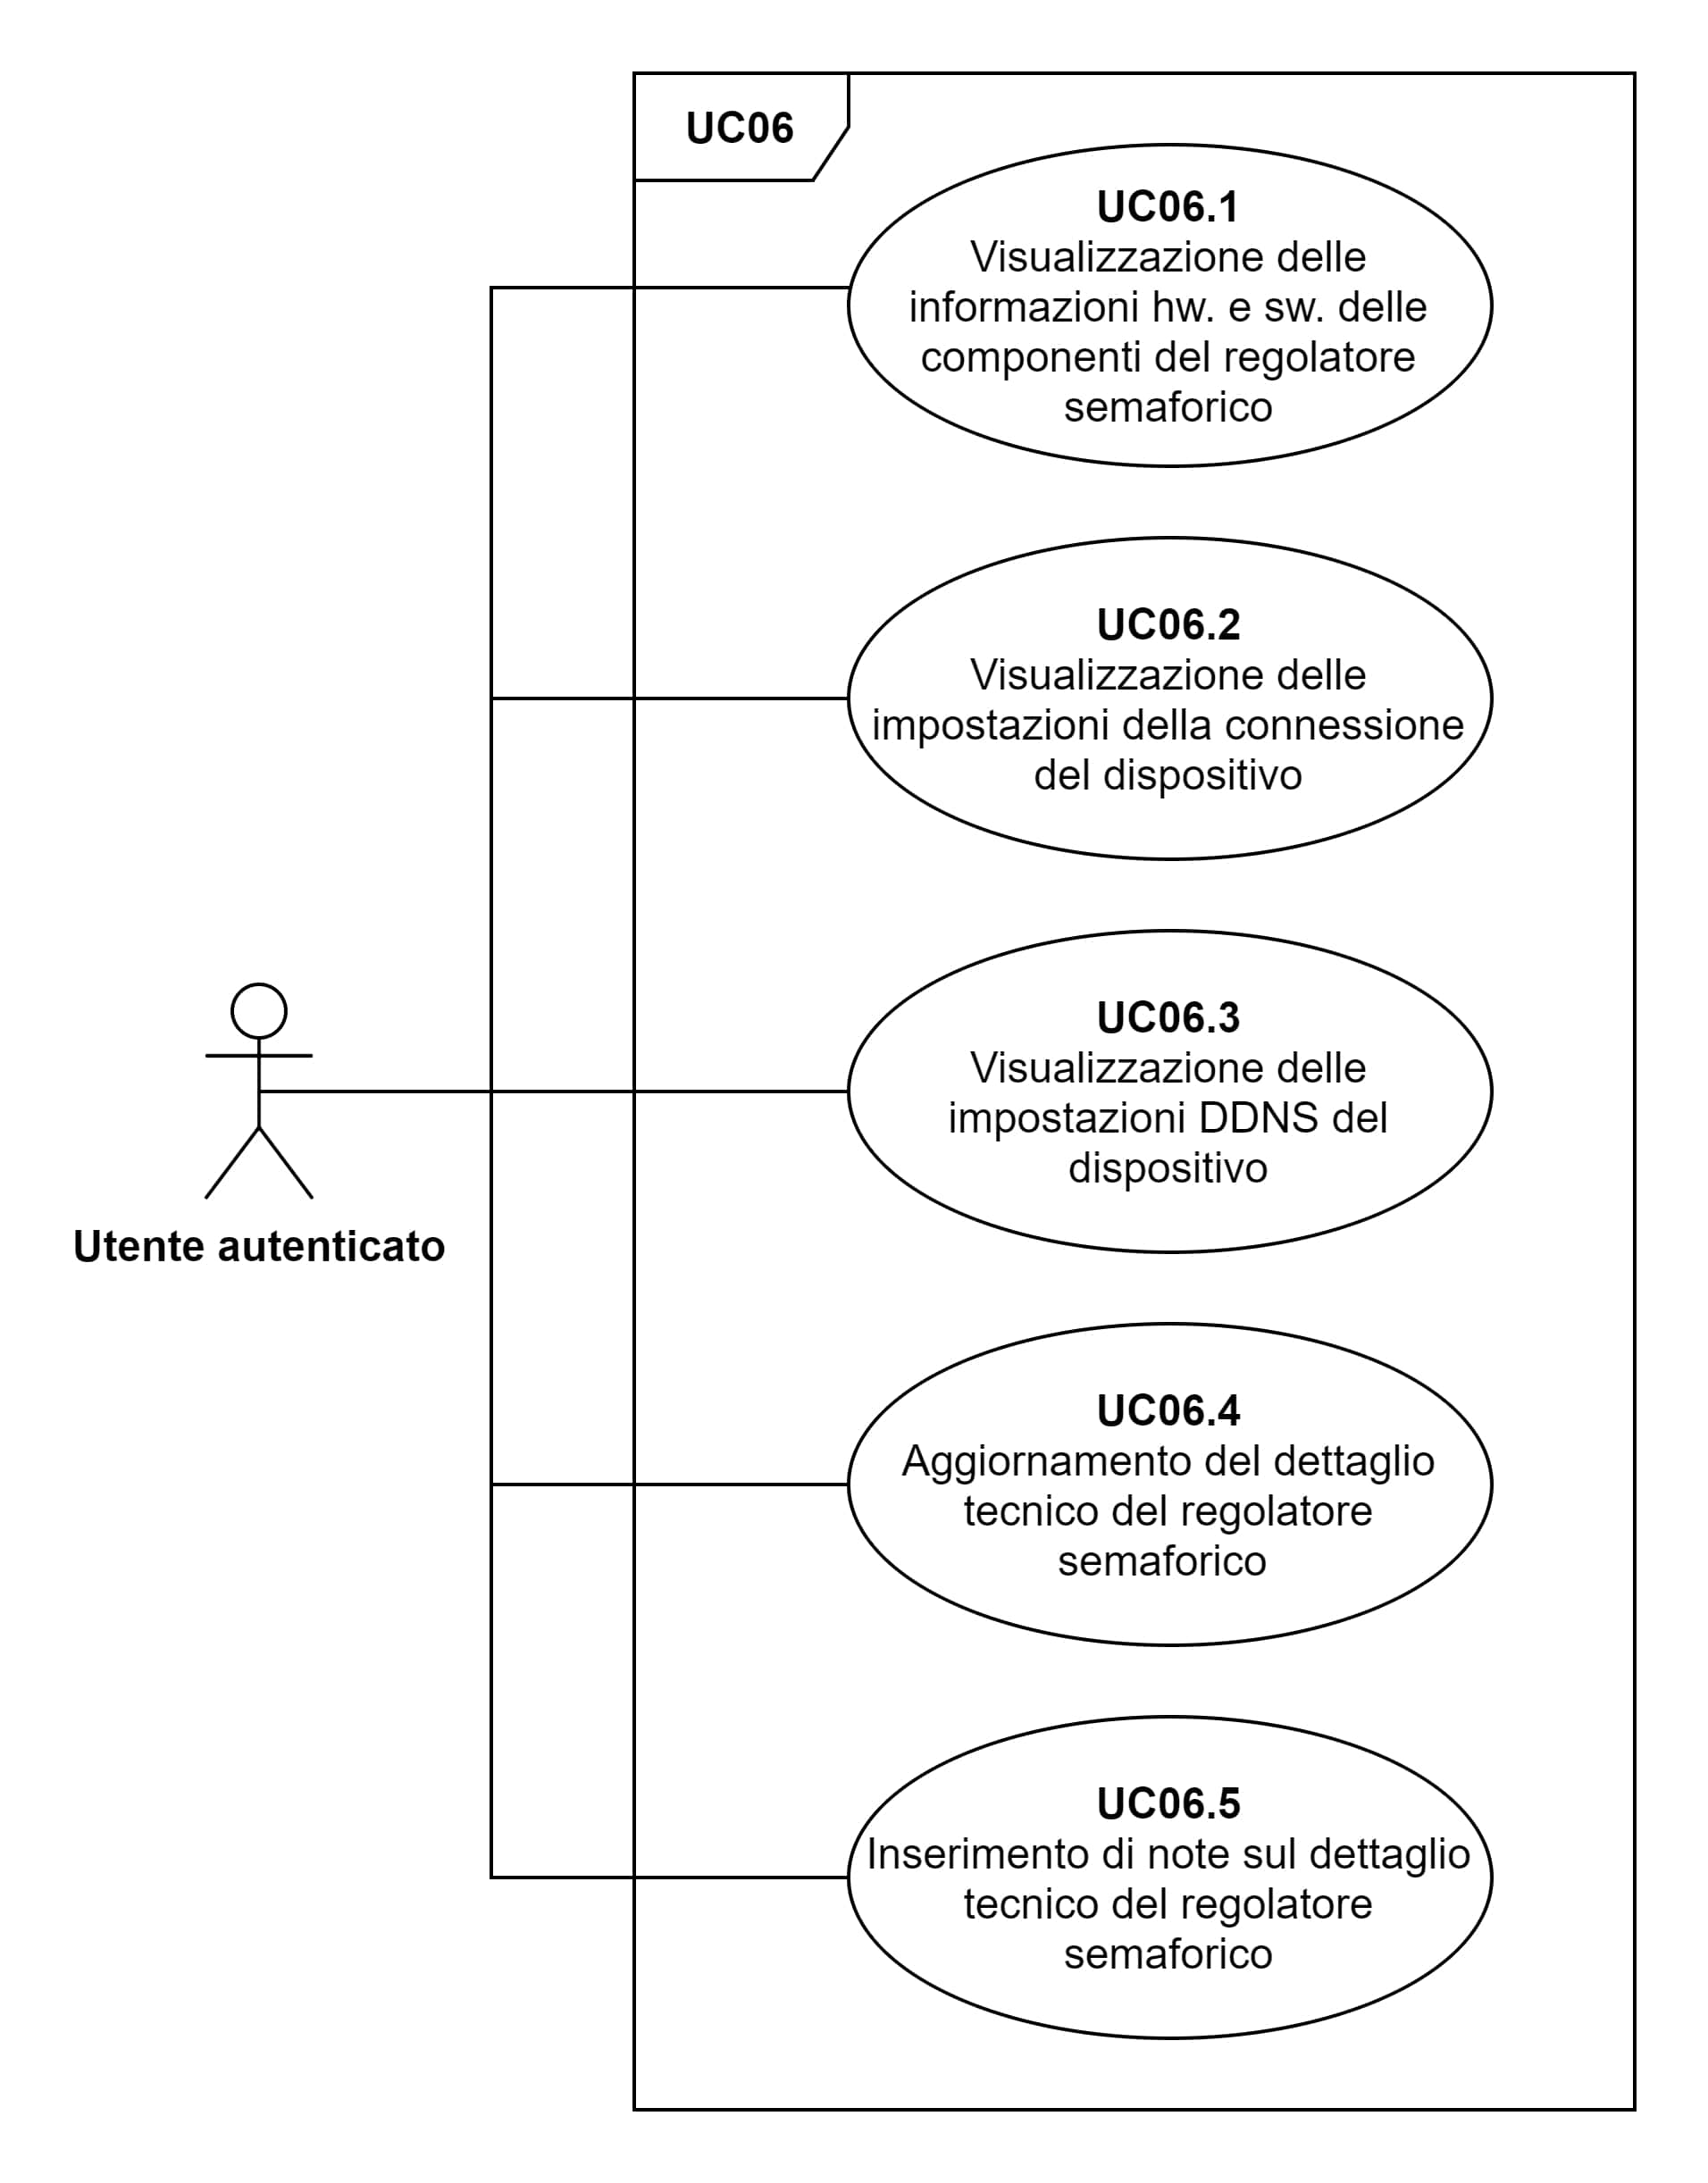
\includegraphics[width=1.0\columnwidth]{appendice-A/uc06} 
    \caption{SMacs - Sotto-casi d'uso di UC06 - Gestione del dettaglio tecnico sul regolatore semaforico}
\end{figure}

\begin{usecase}{06.1}{Visualizzazione delle informazioni hardware e software delle componenti del regolatore semaforico}
\usecaseprimaryactors{Utente autenticato}
\usecasepre{L'utente sta visionando il dettaglio tecnico del regolatore semaforico.}
\usecasedesc{Vengono visualizzate le informazioni hardware e software delle componenti del regolatore semaforico.}
\usecasepost{Vengono visualizzate le informazioni hardware e software delle componenti del regolatore semaforico.}
\label{uc:UC06-1}
\end{usecase}

\begin{usecase}{06.2}{Visualizzazione delle impostazioni della connessione del dispositivo}
\usecaseprimaryactors{Utente autenticato}
\usecasepre{L'utente sta visionando il dettaglio tecnico del regolatore semaforico.}
\usecasedesc{Vengono visualizzati l'indirizzo IP e la porta a cui il dispositivo è raggiungibile.}
\usecasepost{Vengono visualizzati l'indirizzo IP e la porta a cui il dispositivo è raggiungibile.}
\label{uc:UC06-2}
\end{usecase}

\begin{usecase}{06.3}{Visualizzazione delle impostazioni DDNS del dispositivo}
\usecaseprimaryactors{Utente autenticato}
\usecasepre{L'utente sta visionando il dettaglio tecnico del regolatore semaforico.}
\usecasedesc{Vengono visualizzate le impostazioni DDNS del dispositivo.}
\usecasepost{Vengono visualizzate le impostazioni DDNS del dispositivo.}
\label{uc:UC06-3}
\end{usecase}

\begin{usecase}{06.4}{Aggiornamento del dettaglio tecnico del regolatore semaforico}
\usecaseprimaryactors{Utente autenticato}
\usecasepre{L'utente sta visionando il dettaglio tecnico del regolatore semaforico.}
\usecasedesc{L'utente seleziona la funzionalità di aggiornamento e viene aggiornato il dettaglio tecnico del regolatore semaforico.}
\usecasepost{L'utente seleziona la funzionalità di aggiornamento e viene aggiornato il dettaglio tecnico del regolatore semaforico.}
\label{uc:UC06-4}
\end{usecase}

\begin{usecase}{06.5}{Inserimento di note sul dettaglio tecnico del regolatore semaforico}
\usecaseprimaryactors{Utente autenticato}
\usecasepre{L'utente sta visionando il dettaglio tecnico del regolatore semaforico.}
\usecasedesc{L'utente seleziona la funzionalità di inserimento di note sul dettaglio tecnico del regolatore semaforico e inserisce delle note.}
\usecasepost{L'utente seleziona la funzionalità di inserimento di note sul dettaglio tecnico del regolatore semaforico e inserisce delle note.}
\label{uc:UC06-5}
\end{usecase}

\begin{usecase}{07}{Gestione del regolatore semaforico}
\usecaseprimaryactors{Utente autenticato}
\usecasepre{L'utente sta visionando il dettaglio del regolatore semaforico selezionato dalla lista.}
\usecasedesc{L'utente può gestire il funzionamento del regolatore semaforico.}
\usecasepost{L'utente può gestire il funzionamento del regolatore semaforico.}
\label{uc:UC07}
\end{usecase}

\begin{figure}[!h] 
    \centering 
    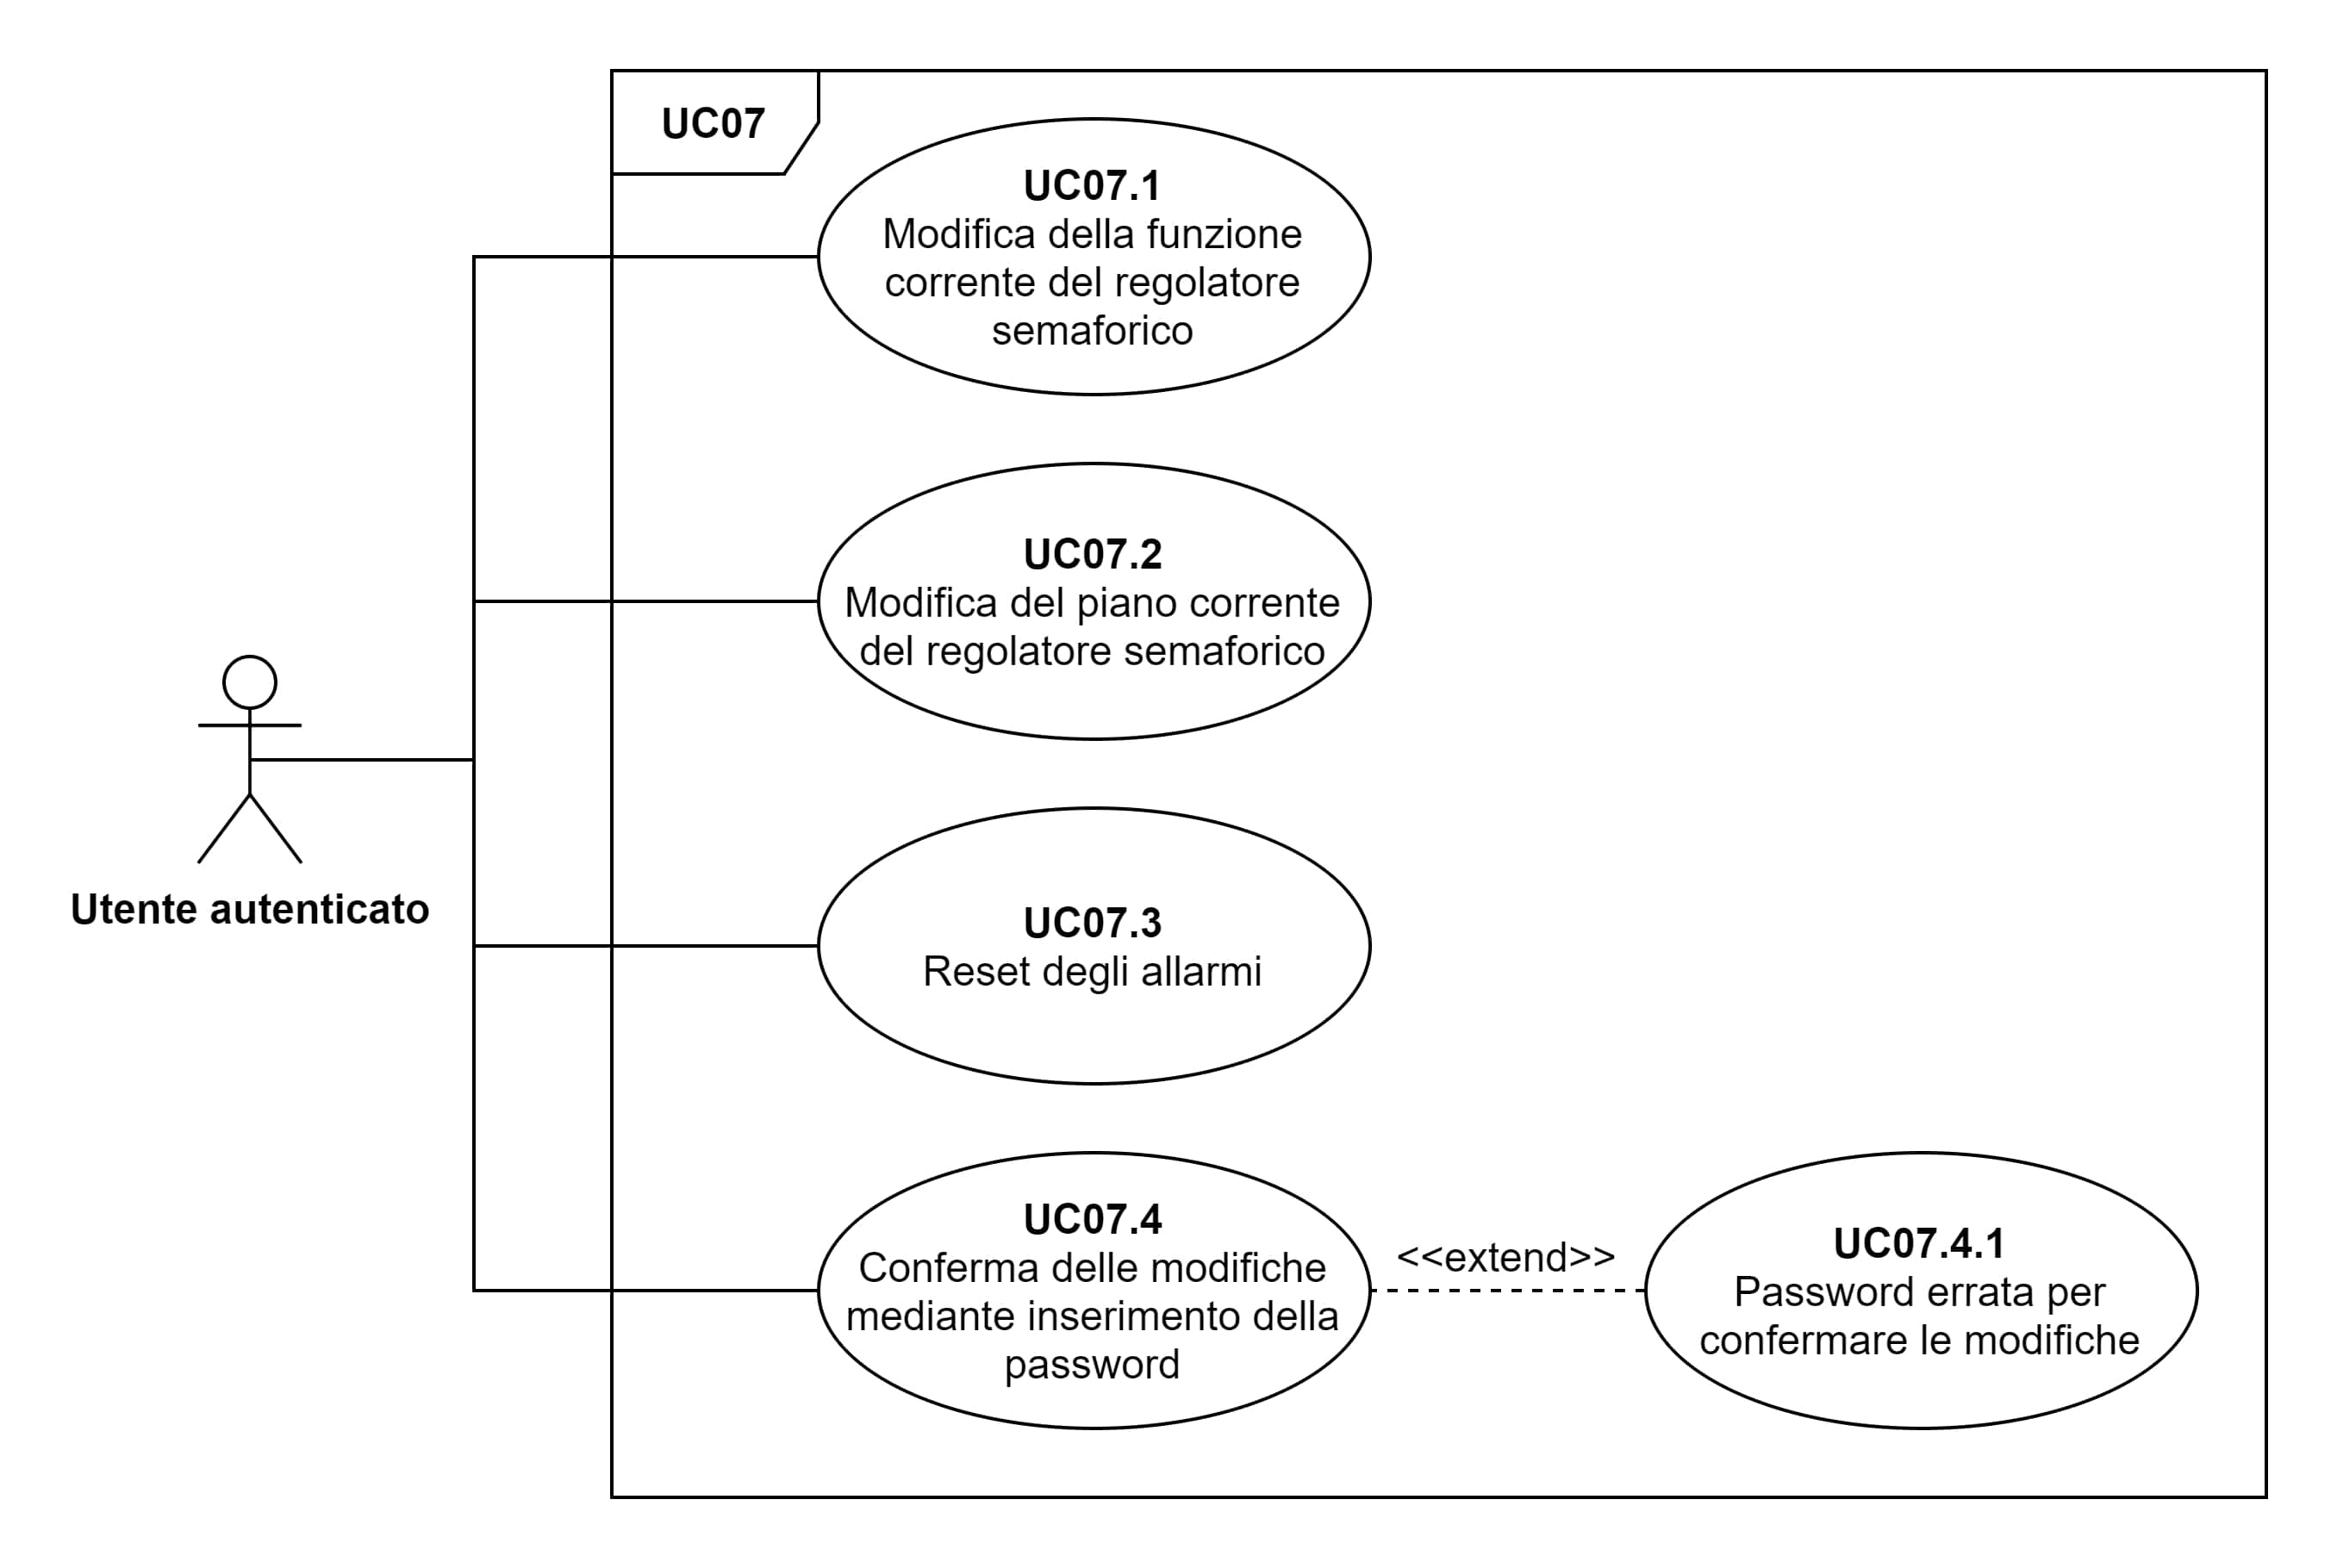
\includegraphics[width=1.0\columnwidth]{appendice-A/uc07} 
    \caption{SMacs - Sotto-casi d'uso di UC07 - Gestione del regolatore semaforico}
\end{figure}

\begin{usecase}{07.1}{Modifica della funzione corrente del regolatore semaforico}
\usecaseprimaryactors{Utente autenticato}
\usecasepre{L'utente ha a disposizione le funzionalità di gestione del regolatore semaforico.}
\usecasedesc{L'utente ha selezionato la funzionalità di modifica e ha aggiornato la funzione corrente del regolatore semaforico.}
\usecasepost{L'utente ha selezionato la funzionalità di modifica e ha aggiornato la funzione corrente del regolatore semaforico.}
\label{uc:UC07-1}
\end{usecase}

\begin{usecase}{07.2}{Modifica del piano corrente del regolatore semaforico}
\usecaseprimaryactors{Utente autenticato}
\usecasepre{L'utente ha a disposizione le funzionalità di gestione del regolatore semaforico.}
\usecasedesc{L'utente ha selezionato la funzionalità di modifica e ha aggiornato il piano corrente del regolatore semaforico.}
\usecasepost{L'utente ha selezionato la funzionalità di modifica e ha aggiornato il piano corrente del regolatore semaforico.}
\label{uc:UC07-2}
\end{usecase}

\begin{usecase}{07.3}{Reset degli allarmi}
\usecaseprimaryactors{Utente autenticato}
\usecasepre{L'utente ha a disposizione le funzionalità di gestione del regolatore semaforico.}
\usecasedesc{L'utente ha selezionato la funzionalità di reset e ha resettato gli allarmi relativi al regolatore semaforico attualmente registrati per il dispositivo.}
\usecasepost{L'utente ha selezionato la funzionalità di reset e ha resettato gli allarmi relativi al regolatore semaforico attualmente registrati per il dispositivo.}
\label{uc:UC07-3}
\end{usecase}

\begin{usecase}{07.4}{Conferma delle modifiche mediante inserimento della password}
\usecaseprimaryactors{Utente autenticato}
\usecasepre{L'utente ha modificato un'impostazione del regolatore semaforico.}
\usecasedesc{L'utente ha modificato un dato di funzionamento del regolatore semaforico e per confermarlo deve inserire la propria password.}
\usecasepost{L'utente ha modificato un dato di funzionamento del regolatore semaforico e per confermarlo ha inserito la propria password.}
\usecaseext{UC07.4.1}
\label{uc:UC07-4}
\end{usecase}

\begin{usecase}{07.4.1}{Password errata per confermare le modifiche}
\usecaseprimaryactors{Utente autenticato}
\usecasepre{L'utente ha inserito la propria password per confermare le modifiche.}
\usecasedesc{L'utente ha inserito una password errata, la modifica non viene confermata e viene avvisato con un messaggio di errore.}
\usecasepost{L'utente ha inserito una password errata, la modifica non viene confermata e viene avvisato con un messaggio di errore.}
\label{uc:UC07-4-1}
\end{usecase}

\begin{usecase}{08}{Lista degli eventi del regolatore semaforico}
\usecaseprimaryactors{Utente autenticato}
\usecasepre{L'utente sta visionando il dettaglio del regolatore semaforico selezionato dalla lista.}
\usecasedesc{Viene visualizzata la lista degli eventi relativi al regolatore semaforico selezionato per la data corrente.}
\usecasepost{Viene visualizzata la lista degli eventi relativi al regolatore semaforico selezionato per la data corrente.}
\label{uc:UC08}
\end{usecase}

\begin{figure}[!h] 
    \centering 
    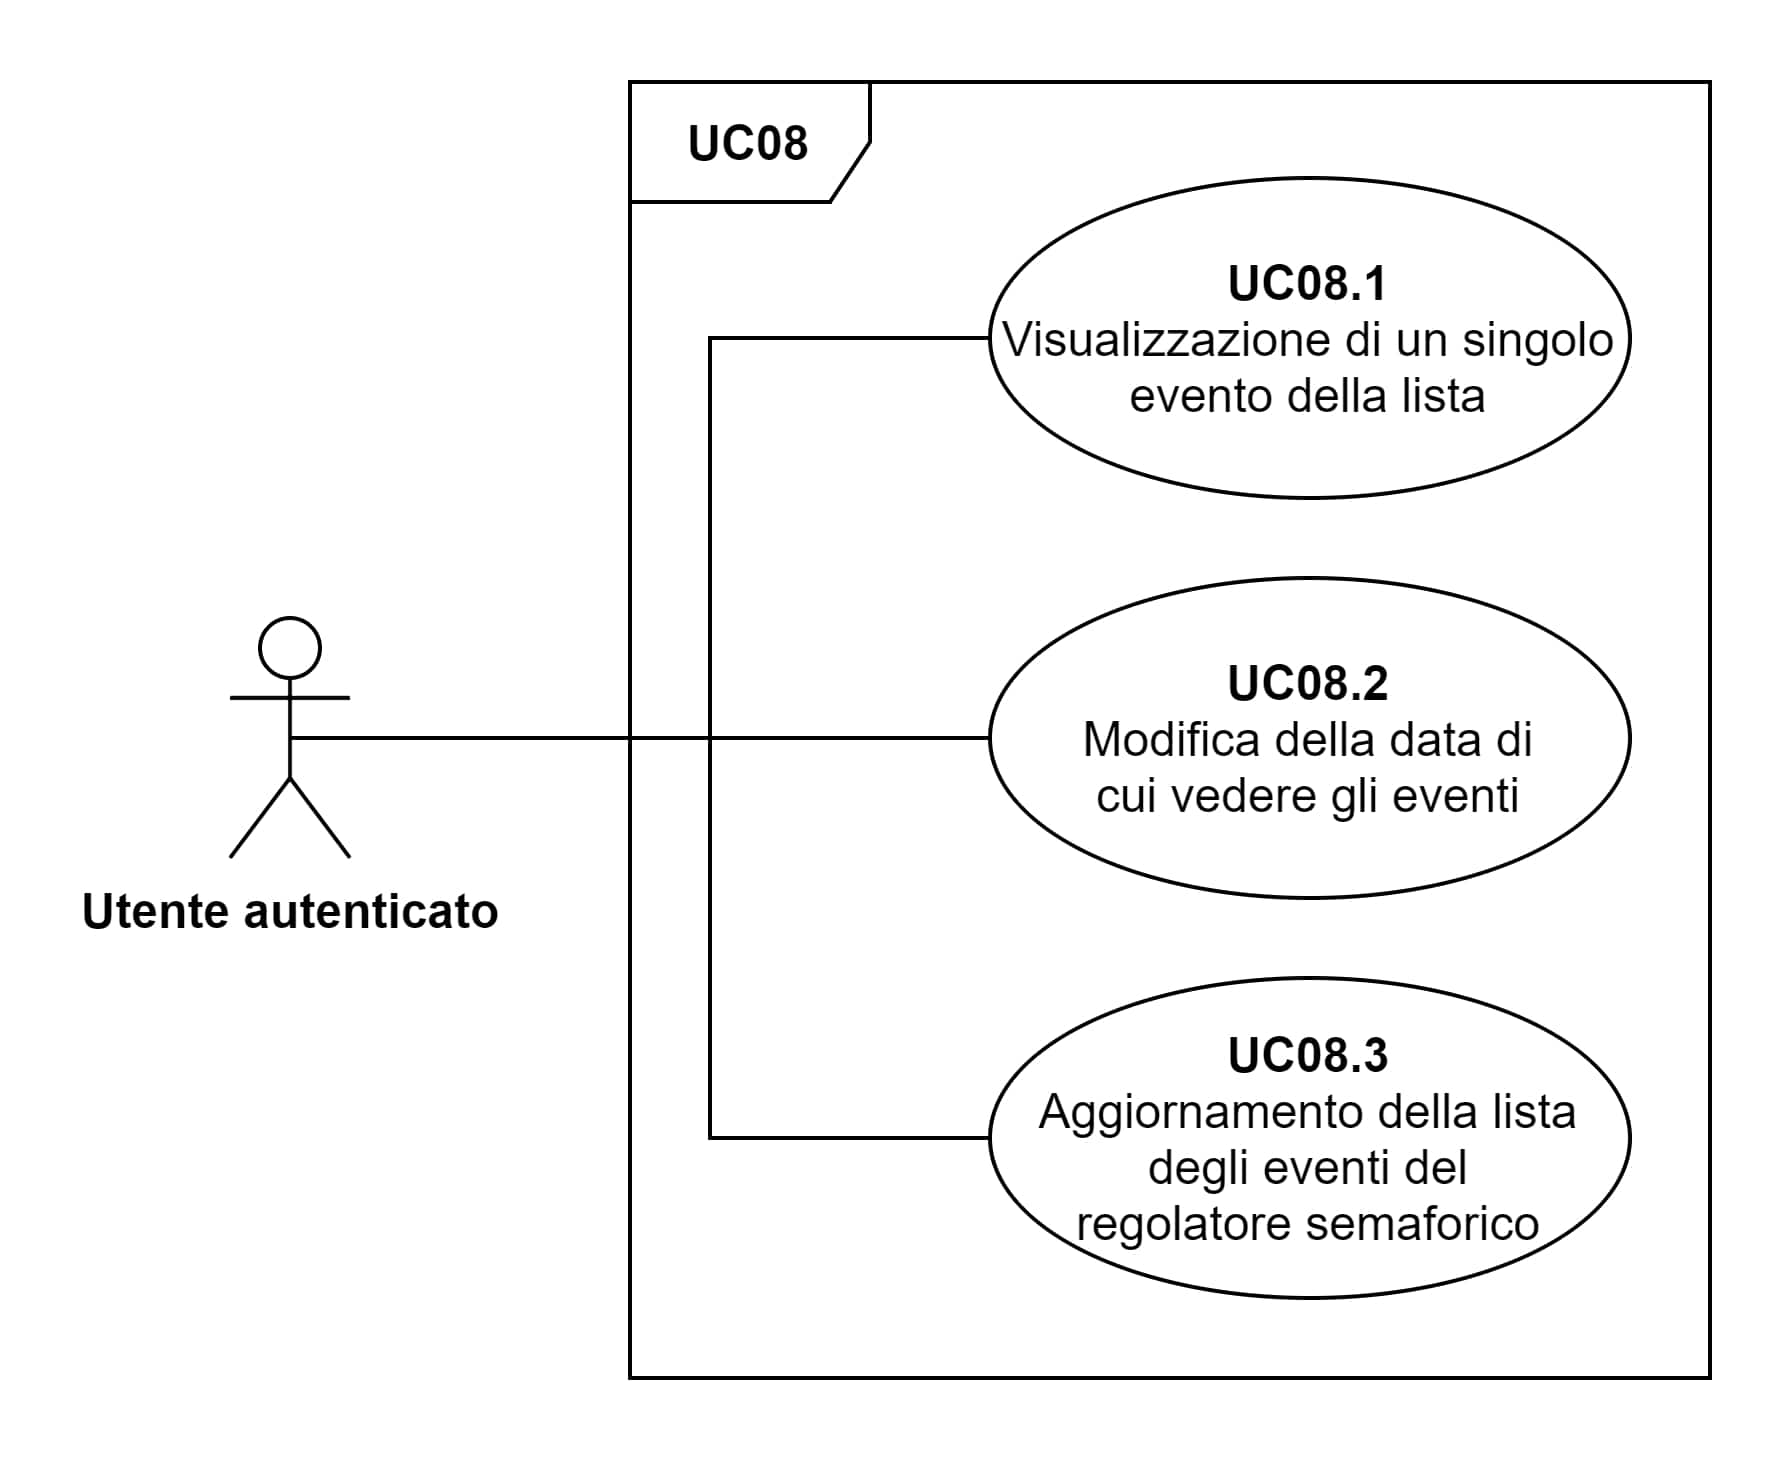
\includegraphics[width=1.0\columnwidth]{appendice-A/uc08} 
    \caption{SMacs - Sotto-casi d'uso di UC08 - Lista degli eventi del regolatore semaforico}
\end{figure}

\begin{usecase}{08.1}{Visualizzazione di un singolo evento della lista}
\usecaseprimaryactors{Utente autenticato}
\usecasepre{L'utente sta visionando la lista degli eventi del regolatore semaforico.}
\usecasedesc{Viene visualizzato un singolo evento relativo al regolatore semaforico della lista, mostrando un icona che rappresenta la gravità dell'evento e un breve messaggio descrittivo.}
\usecasepost{Viene visualizzato un singolo evento relativo al regolatore semaforico della lista, mostrando un icona che rappresenta la gravità dell'evento e un breve messaggio descrittivo.}
\label{uc:UC08-1}
\end{usecase}

\begin{usecase}{08.2}{Modifica della data di cui vedere gli eventi}
\usecaseprimaryactors{Utente autenticato}
\usecasepre{L'utente sta visionando la lista degli eventi del regolatore semaforico.}
\usecasedesc{L'utente seleziona la funzionalità di aggiornamento e aggiorna la data di visualizzazione degli eventi del regolatore semaforico.}
\usecasepost{L'utente seleziona la funzionalità di aggiornamento e aggiorna la data di visualizzazione degli eventi del regolatore semaforico.}
\label{uc:UC08-2}
\end{usecase}

\begin{usecase}{08.3}{Aggiornamento della lista degli eventi del regolatore semaforico}
\usecaseprimaryactors{Utente autenticato}
\usecasepre{L'utente sta visionando la lista degli eventi del regolatore semaforico.}
\usecasedesc{L'utente seleziona la funzionalità di aggiornamento e viene aggiornata la lista degli eventi del regolatore semaforico.}
\usecasepost{L'utente seleziona la funzionalità di aggiornamento e viene aggiornata la lista degli eventi del regolatore semaforico.}
\label{uc:UC08-3}
\end{usecase}

\begin{usecase}{09}{Visualizzazione del foglio di informazioni del dispositivo}
\usecaseprimaryactors{Utente autenticato}
\usecasepre{L'utente sta visionando il dettaglio del regolatore semaforico selezionato dalla lista.}
\usecasedesc{L'utente ha selezionato la funzionalità di visualizzazione del documento con le informazioni sul dispositivo che viene quindi mostrato.}
\usecasepost{L'utente ha selezionato la funzionalità di visualizzazione del documento con le informazioni sul dispositivo che viene quindi mostrato.}
\label{uc:UC09}
\end{usecase}

\begin{usecase}{10}{Visualizzazione posizione geografica del regolatore semaforico}
\usecaseprimaryactors{Utente autenticato}
\usecasesecondaryactors{Mappe del dispositivo}
\usecasepre{L'utente sta visionando il dettaglio del regolatore semaforico selezionato dalla lista.}
\usecasedesc{L'utente ha selezionato la funzionalità di visualizzazione della posizione geografica del regolatore semaforico e viene quindi reindirizzato all'applicazione di default delle mappe del dispositivo (smartphone/tablet) che visualizzerà quanto richiesto.}
\usecasepost{L'utente ha selezionato la funzionalità di visualizzazione della posizione geografica del regolatore semaforico e viene quindi reindirizzato all'applicazione di default delle mappe del dispositivo (smartphone/tablet) che visualizzerà quanto richiesto.}
\label{uc:UC10}
\end{usecase}

\begin{usecase}{11}{Visualizzazione di un testo riassuntivo sullo stato dei dispositivi}
\usecaseprimaryactors{Utente autenticato}
\usecasepre{L'utente ha ricevuto una notifica: quindi ha avviato l'applicazione oppure la stava già utilizzando (in qualsiasi modo).}
\usecasedesc{L'utente ha selezionato la funzionalità di visualizzazione di un testo riassuntivo della situazione attuale dello stato dei dispositivi collegati al suo account, mostrando anche i problemi (messaggi di diagnostica) presenti nuovi, presenti passati, risolti.}
\usecasepost{L'utente ha selezionato la funzionalità di visualizzazione di un testo riassuntivo della situazione attuale dello stato dei dispositivi collegati al suo account, mostrando anche i problemi (messaggi di diagnostica) presenti nuovi, presenti passati, risolti.}
\label{uc:UC11}
\end{usecase}

\begin{usecase}{12}{Gestione dell'intervallo di aggiornamento dati}
\usecaseprimaryactors{Utente autenticato}
\usecasepre{L'utente sta visionando la lista dei dispositivi collegati al proprio profilo.}
\usecasedesc{L'utente ha selezionato la funzionalità di gestione dell'intervallo di aggiornamento dati e ha aggiornato l'intervallo.}
\usecasepost{L'utente ha selezionato la funzionalità di gestione dell'intervallo di aggiornamento dati e ha aggiornato l'intervallo.}
\label{uc:UC12}
\end{usecase}

\begin{usecase}{13}{Informazioni sull'app}
\usecaseprimaryactors{Utente autenticato}
\usecasepre{L'utente sta visionando la lista dei dispositivi collegati al proprio profilo.}
\usecasedesc{L'utente ha selezionato la funzionalità di visualizzazione delle informazioni sull'applicazione e di cui viene visualizzata la versione e la data di rilascio, il server a cui si è connessi e l'username.}
\usecasepost{L'utente ha selezionato la funzionalità di visualizzazione delle informazioni sull'applicazione e di cui viene visualizzata la versione e la data di rilascio, il server a cui si è connessi e l'username.}
\label{uc:UC13}
\end{usecase}

\begin{usecase}{14}{Gestione della modalità di debug}
\usecaseprimaryactors{Utente autenticato}
\usecasepre{L'utente sta visionando la lista dei dispositivi collegati al proprio profilo.}
\usecasedesc{L'utente ha selezionato la funzionalità di gestione della modalità di debug e può attivarla o disattivarla, visionando dove i dati di debug verranno salvati.}
\usecasepost{L'utente ha selezionato la funzionalità di gestione della modalità di debug e può attivarla o disattivarla, visionando dove i dati di debug verranno salvati.}
\label{uc:UC14}
\end{usecase}

\begin{usecase}{15}{Logout dal sistema}
\usecaseprimaryactors{Utente autenticato}
\usecasepre{L'utente ha la possibilità di tornare un utente non autenticato.}
\usecasedesc{L'utente ha selezionato la funzionalità di logout e viene quindi disconnesso dal sistema.}
\usecasepost{L'utente ha selezionato la funzionalità di logout e viene quindi disconnesso dal sistema.}
\label{uc:UC15}
\end{usecase}

% \section{Tracciamento dei requisiti}

% Da un'attenta analisi dei requisiti e dei casi d'uso effettuata sul progetto è stata stilata la tabella che traccia i requisiti in rapporto ai casi d'uso.\\
% Sono stati individuati diversi tipi di requisiti e si è quindi fatto utilizzo di un codice identificativo per distinguerli.\\
% Il codice dei requisiti ha la forma $R\alpha{}x$ con $x$ numero naturale progressivo mentre $\alpha$ può essere:
% \begin{itemize}
%     \item F, che indica un requisito funzionale e obbligatorio, ovvero che implementa una funzionalità obbligatoria per il corretto funzionamento e completamento del prodotto;
%     \item D, che indica nuovamente un requisito funzionale ma desiderabile, ovvero che implementa una funzionalità che offre valore aggiunto ma che senza il prodotto può comunque portare a termine gli obiettivi per cui è stato creato;
%     \item Z, che indica ancora una volta un requisito funzionale però opzionale, ovvero che offre valore aggiunto ma che è subordinato dalla realizzazione degli altri requisiti, ed è quindi di inferiore importanza;
%     \item Q, che indica un requisito qualitativo, ovvero che garantisce un corretto funzionamento del prodotto secondo le attese dell'utente e degli stakeholder;
%     \item V, che indica un requisito vincolante per la buona riuscita del progetto e del prodotto, senza il cui completamento il prodotto non può ritenersi concluso.
% \end{itemize}
% Nelle tabelle \ref{tab:requisiti-funzionali}, \ref{tab:requisiti-qualitativi} e \ref{tab:requisiti-vincolo} sono riassunti i requisiti e il loro tracciamento con i casi d'uso delineati in fase di analisi.

% \newpage

% \begin{table}%
% \caption{Tabella del tracciamento dei requisiti funzionali}
% \label{tab:requisiti-funzionali}
% \begin{tabularx}{\textwidth}{lXl}
% \hline\hline
% \textbf{Requisito} & \textbf{Descrizione} & \textbf{Use Case}\\
% \hline
% RF01 & Viene visualizzata la schermata iniziale dell'applicazione quando l'utente non autenticato accede all'applicazione. & UC01 \\
% RF02 & Quando l'utente non autenticato si trova nella schermata iniziale dell'applicazione viene visualizzato il link per accedere al sito web dell'azienda. & UC01.1 \\
% RF03 & Quando l'utente non autenticato si trova nella schermata iniziale dell'applicazione viene visualizzato il modulo per contattare il servizio clienti. & UC01.2 \\
% RF04 & Quando l'utente non autenticato si trova nella schermata iniziale dell'applicazione viene visualizzato il link per accedere al sito web dell'azienda di cui è partner. & UC01.3 \\
% RF05 & Quando l'utente non autenticato si trova nella schermata iniziale dell'applicazione viene visualizzato la funzionalità di accesso alla schermata di autenticazione. & UC01.4 \\
% RF06 & L'utente non autenticato può autenticarsi presso il sistema. & UC02 \\
% RF07 & L'utente non autenticato può inserire il nome del server a cui connettersi. & UC02.1 \\
% RF08 & L'utente non autenticato può inserire il proprio nome utente per connettersi al sistema. & UC02.2 \\
% RF09 & L'utente non autenticato può inserire la propria password per connettersi al sistema. & UC02.3 \\
% RF10 & Se l'utente non autenticato si è dimenticato la propria password può accedere alla pagina web per contattare il servizio clienti. & UC02.4 \\
% RF11 & Se l'utente non autenticato ha inserito un server che non è valido viene visualizzato un messaggio di errore. & UC02.5 \\
% RF12 & Se l'utente non autenticato ha inserito delle credenziali che non sono valide viene visualizzato un messaggio di errore. & UC02.6 \\
% RF13 & L'utente autenticato può visionare la lista dei dispositivi di cui ha il permesso di gestione. & UC03 \\
% RF14 & L'utente autenticato può visionare un elemento della lista dei dispositivi comprensivo di un dettaglio compatto. & UC03.1 \\
% RF15 & L'utente autenticato è notificato quando la lista dei dispositivi di cui ha il permesso di gestione è vuota. & UC03.2 \\
% RF16 & L'utente autenticato può visionare la lista dei dispositivi di cui ha il permesso di gestione in ordine alfabetico. & UC03.3 \\
% RF17 & L'utente autenticato può visionare la lista dei soli dispositivi di cui ha il permesso di gestione che hanno segnalazioni (di malfunzionamento). & UC03.4 \\
% RF18 & L'utente autenticato può visionare la lista dei dispositivi entro il raggio di 1 Km dalla propria posizione di cui ha il permesso di gestione. & UC03.5 \\
% RF19 & L'utente autenticato può visionare la lista dei dispositivi filtrati in base a una ricerca testuale di cui ha il permesso di gestione. & UC03.6 \\
% RF20 & L'utente autenticato può aggiornare la lista dei dispositivi di cui ha il permesso di gestione ottenendone una nuova copia dal sistema. & UC03.7 \\
% RF21 & L'utente autenticato può ottenere informazioni dettagliate sullo stato di un regolatore semaforico. & UC04 \\
% RF22 & L'utente autenticato può ottenere informazioni sulla massima gravità fra i messaggi di diagnostica attivi nel dispositivo. & UC04.1 \\
% RF23 & L'utente autenticato può ottenere informazioni sullo stato del regolatore semaforico (funzione, livello). & UC04.2 \\
% RF24 & L'utente autenticato può ottenere informazioni sullo stato dei gruppi semaforici del regolatore semaforico. & UC04.3 \\
% RF25 & L'utente autenticato può ottenere informazioni sullo stato degli input presenti nel regolatore semaforico. & UC04.4 \\
% RF26 & L'utente autenticato può ottenere la data in cui è avvenuto l'ultimo aggiornamento dei dati del regolatore semaforico. & UC04.5 \\
% RF27 & L'utente autenticato può ottenere i messaggi di diagnostica presenti nel regolatore semaforico. & UC04.6 \\
% RF28 & L'utente autenticato può aggiornare lo stato del regolatore semaforico. & UC04.7 \\
% RF29 & L'utente autenticato può visionare il sinottico del regolatore semaforico. & UC05 \\
% RF30 & L'utente autenticato può gestire il dettaglio tecnico sul regolatore semaforico. & UC06 \\
% RF31 & L'utente autenticato può ottenere delle informazioni hardware e software delle componenti del regolatore semaforico. & UC06.1 \\
% RF32 & L'utente autenticato può ottenere informazioni sulla modalità di connessione attiva nel dispositivo. & UC06.2 \\
% RF33 & L'utente autenticato può ottenere informazioni sulle impostazioni DDNS del dispositivo. & UC06.3 \\
% RF34 & L'utente autenticato può aggiornare il dettaglio tecnico del regolatore semaforico. & UC06.4 \\
% RF35 & L'utente autenticato può inserire delle note sul dettaglio tecnico del regolatore semaforico. & UC06.5 \\
% RF36 & L'utente autenticato può gestire il regolatore semaforico. & UC07 \\
% RF37 & L'utente autenticato può modificare la funzione corrente del regolatore semaforico. & UC07.1 \\
% RF38 & L'utente autenticato può modificare il piano corrente del regolatore semaforico. & UC07.2 \\
% RF39 & L'utente autenticato può resettare gli allarmi del regolatore semaforico. & UC07.3 \\
% RF40 & L'utente autenticato può inserire la propria password per confermare le modifiche ai dati del regolatore semaforico. & UC07.4 \\
% RF41 & Se l'utente autenticato ha inserito la password e non corrisponde alla propria viene visualizzato un messaggio di errore. & UC07.4.1 \\
% RF42 & L'utente autenticato può visionare la lista degli eventi del regolatore semaforico. & UC08 \\
% RF43 & L'utente autenticato può visionare un singolo evento della lista. & UC08.1 \\
% RF44 & L'utente autenticato può modificare la data di cui vedere gli eventi del regolatore semaforico. & UC08.2 \\
% RF45 & L'utente autenticato può aggiornare la lista degli eventi del regolatore semaforico. & UC08.3 \\
% RF46 & L'utente autenticato può visionare il foglio contenente informazioni sul dispositivo. & UC09 \\
% RF47 & L'utente autenticato può visionare la posizione geografica del regolatore semaforico. & UC10 \\
% RF48 & L'utente autenticato può visionare un testo riassuntivo sullo stato dei dispositivi previa ricezione di una notifica. & UC11 \\
% RF49 & L'utente autenticato può gestire l'intervallo di aggiornamento dati. & UC12 \\
% RF50 & L'utente autenticato può visionare le informazioni sull'app. & UC13 \\
% RF51 & L'utente autenticato può gestire la modalità di debug. & UC14 \\
% RF52 & L'utente autenticato può effettuare il logout dal sistema. & UC15 \\
% \hline
% \end{tabularx}
% \end{table}%

% \begin{table}%
% \caption{Tabella del tracciamento dei requisiti qualitativi}
% \label{tab:requisiti-qualitativi}
% \begin{tabularx}{\textwidth}{lXl}
% \hline\hline
% \textbf{Requisito} & \textbf{Descrizione} & \textbf{Use Case}\\
% \hline
% RQD-1    & Le prestazioni del simulatore hardware deve garantire la giusta esecuzione dei test e non la generazione di falsi negativi & - \\
% \hline
% \end{tabularx}
% \end{table}%

% \begin{table}%
% \caption{Tabella del tracciamento dei requisiti di vincolo}
% \label{tab:requisiti-vincolo}
% \begin{tabularx}{\textwidth}{lXl}
% \hline\hline
% \textbf{Requisito} & \textbf{Descrizione} & \textbf{Use Case}\\
% \hline
% RVO-1    & La libreria per l'esecuzione dei test automatici deve essere riutilizzabile & - \\
% \hline
% \end{tabularx}
% \end{table}%            % Analisi dei requisiti

%**************************************************************
% Materiale finale
%**************************************************************
\backmatter
\printglossaries
% !TEX encoding = UTF-8
% !TEX TS-program = pdflatex
% !TEX root = ../tesi.tex

%**************************************************************
% Bibliografia
%**************************************************************

\cleardoublepage
\chapter{Bibliografia}

\nocite{*}
% Stampa i riferimenti bibliografici
\printbibliography[heading=subbibliography,title={Riferimenti bibliografici},type=book]

% Stampa i siti web consultati
\printbibliography[heading=subbibliography,title={Siti web consultati},type=online]


\end{document}
